\documentclass[a4paper,11pt]{article} % Formato A4 e fonte de 12pt
\usepackage[utf8]{inputenc} % Suporte para caracteres UTF-8
\usepackage{geometry} % Pacote para ajustar as margens e o formato da página
\usepackage{graphicx} % Para incluir imagens
\usepackage{amsmath} % Pacote para fórmulas matemáticas
\usepackage{hyperref} % Para links e referências
\usepackage{fancyhdr} % Pacote para criar cabeçalhos e rodapés personalizados
\usepackage{listing}
\usepackage{xcolor}

% Configurando margens de 2 cm
\geometry{
  a4paper,
  left=1.5cm,
  right=1.5cm,
  top=2cm,
  bottom=2cm
}

% Configurando o cabeçalho
\pagestyle{fancy}
\fancyhf{}
\fancyhead[L]{Laboratory 03 - Metasploit and Snort} % Cabeçalho à esquerda
\fancyfoot[C]{\thepage} % Número da página no rodapé central

\begin{document}

% Adicionando nome, curso e professor
\begin{flushleft}
    \textbf{Name:} João Pedro Marçal Storino \\
    \textbf{Course:} ICM 2A \\
    \textbf{Subject:} Informatique - Sécurité, Confiance, Confidentialité \\
    \textbf{Professor:} Philippe Jaillon \\
    \textbf{Date:} \today
\end{flushleft}

\noindent\rule{\textwidth}{0.4mm} % Separador horizontal

\tableofcontents
\newpage

% Colocando o título manualmente após a linha
\begin{center}
    {\LARGE \textbf{Metasploit and Snort}} % Título personalizado
\end{center}

\section{Metasploit}
\subsection{Objective}
This Labtainer exercise explores the use of the metasploit tool which is installed on a Kali Linux
system (attacker) and is meant to learn simple penetration skills on a purposely vulnerable
metasploitable host (victim).\\
Note: the attacker computer is configured to have IP address \texttt{192.168.1.3} while the victim
computer is \texttt{192.168.1.2}

\subsection{Starting the Lab}
After we open our \textbf{VM}, in the terminal we write:
\[\texttt{labtainer metasploit}\]
Which opens this two terminal windows, one for the \textbf{Attacker} and one for the \textbf{Victim}:

\begin{figure}[h!]
    \centering
    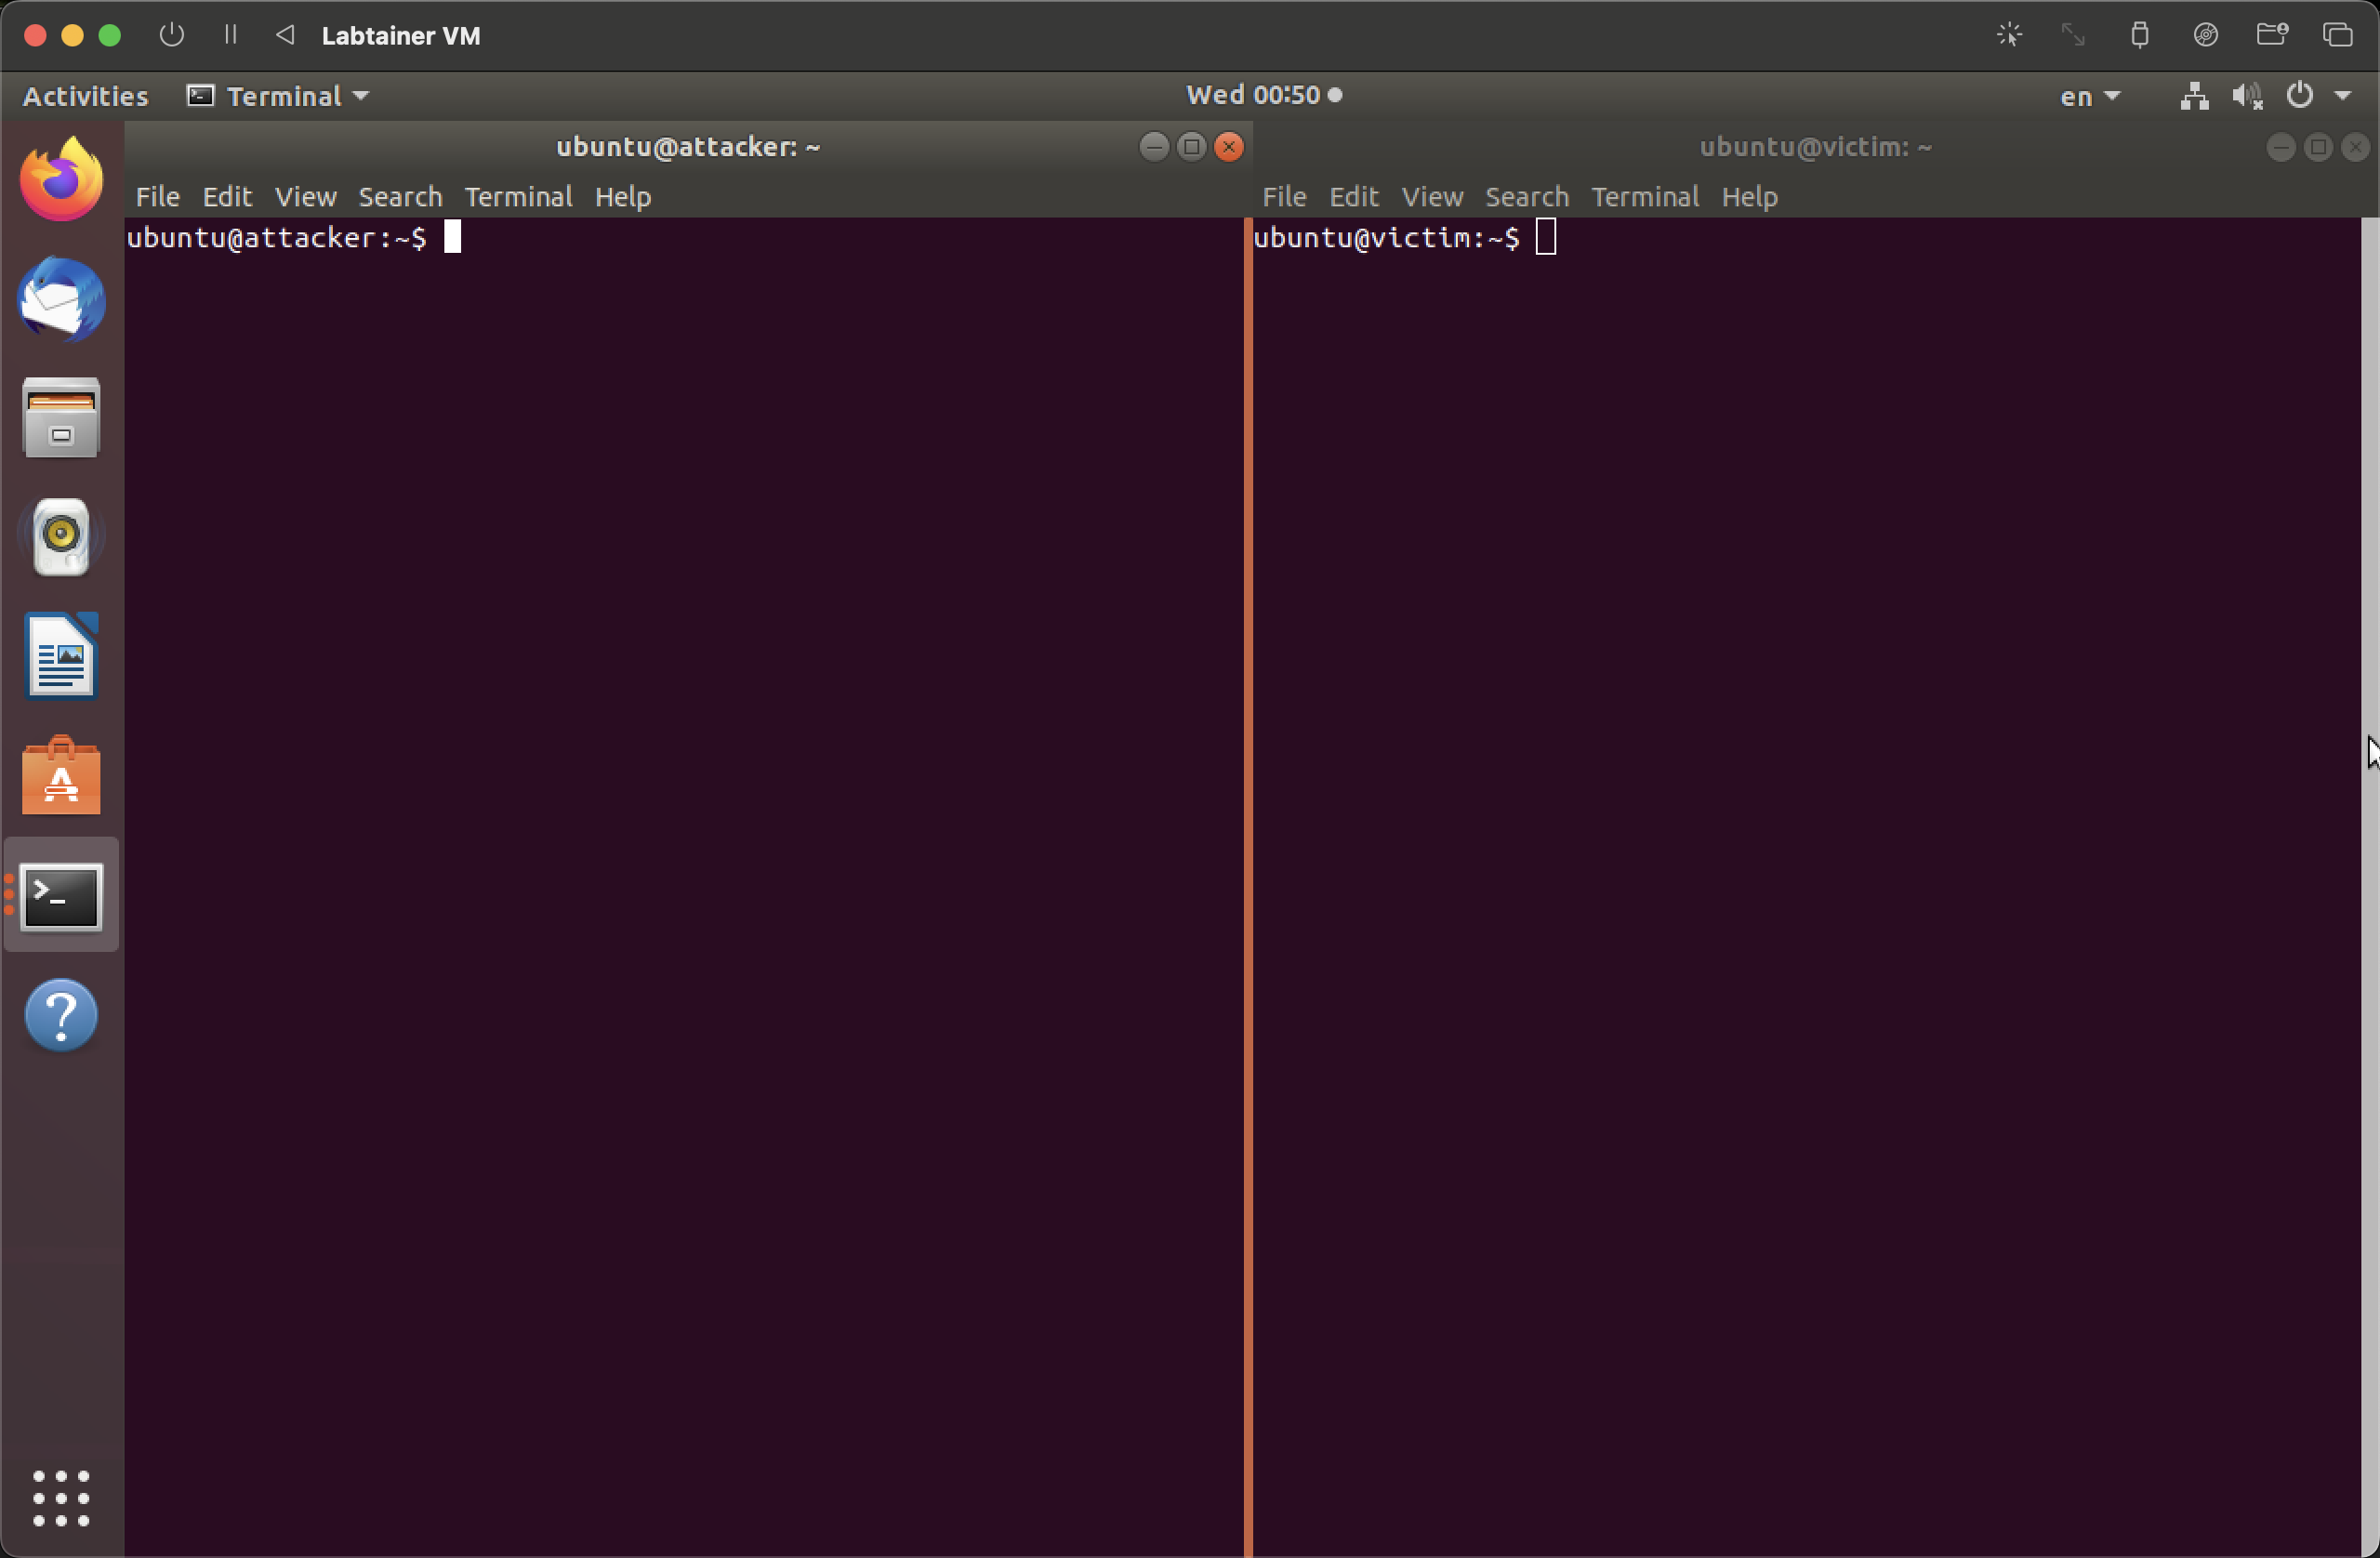
\includegraphics[width=0.7\textwidth]{images/01.png}
    \caption{Attacker and Victim Terminal}
\end{figure}

\subsection{Verifying Connection}
After that, we use the comand below in the attacker terminal to check the connectivity between the attacker and the victim:
\[\texttt{ping 192.168.1.2}\]

\break

\begin{figure}[h!]
    \centering
    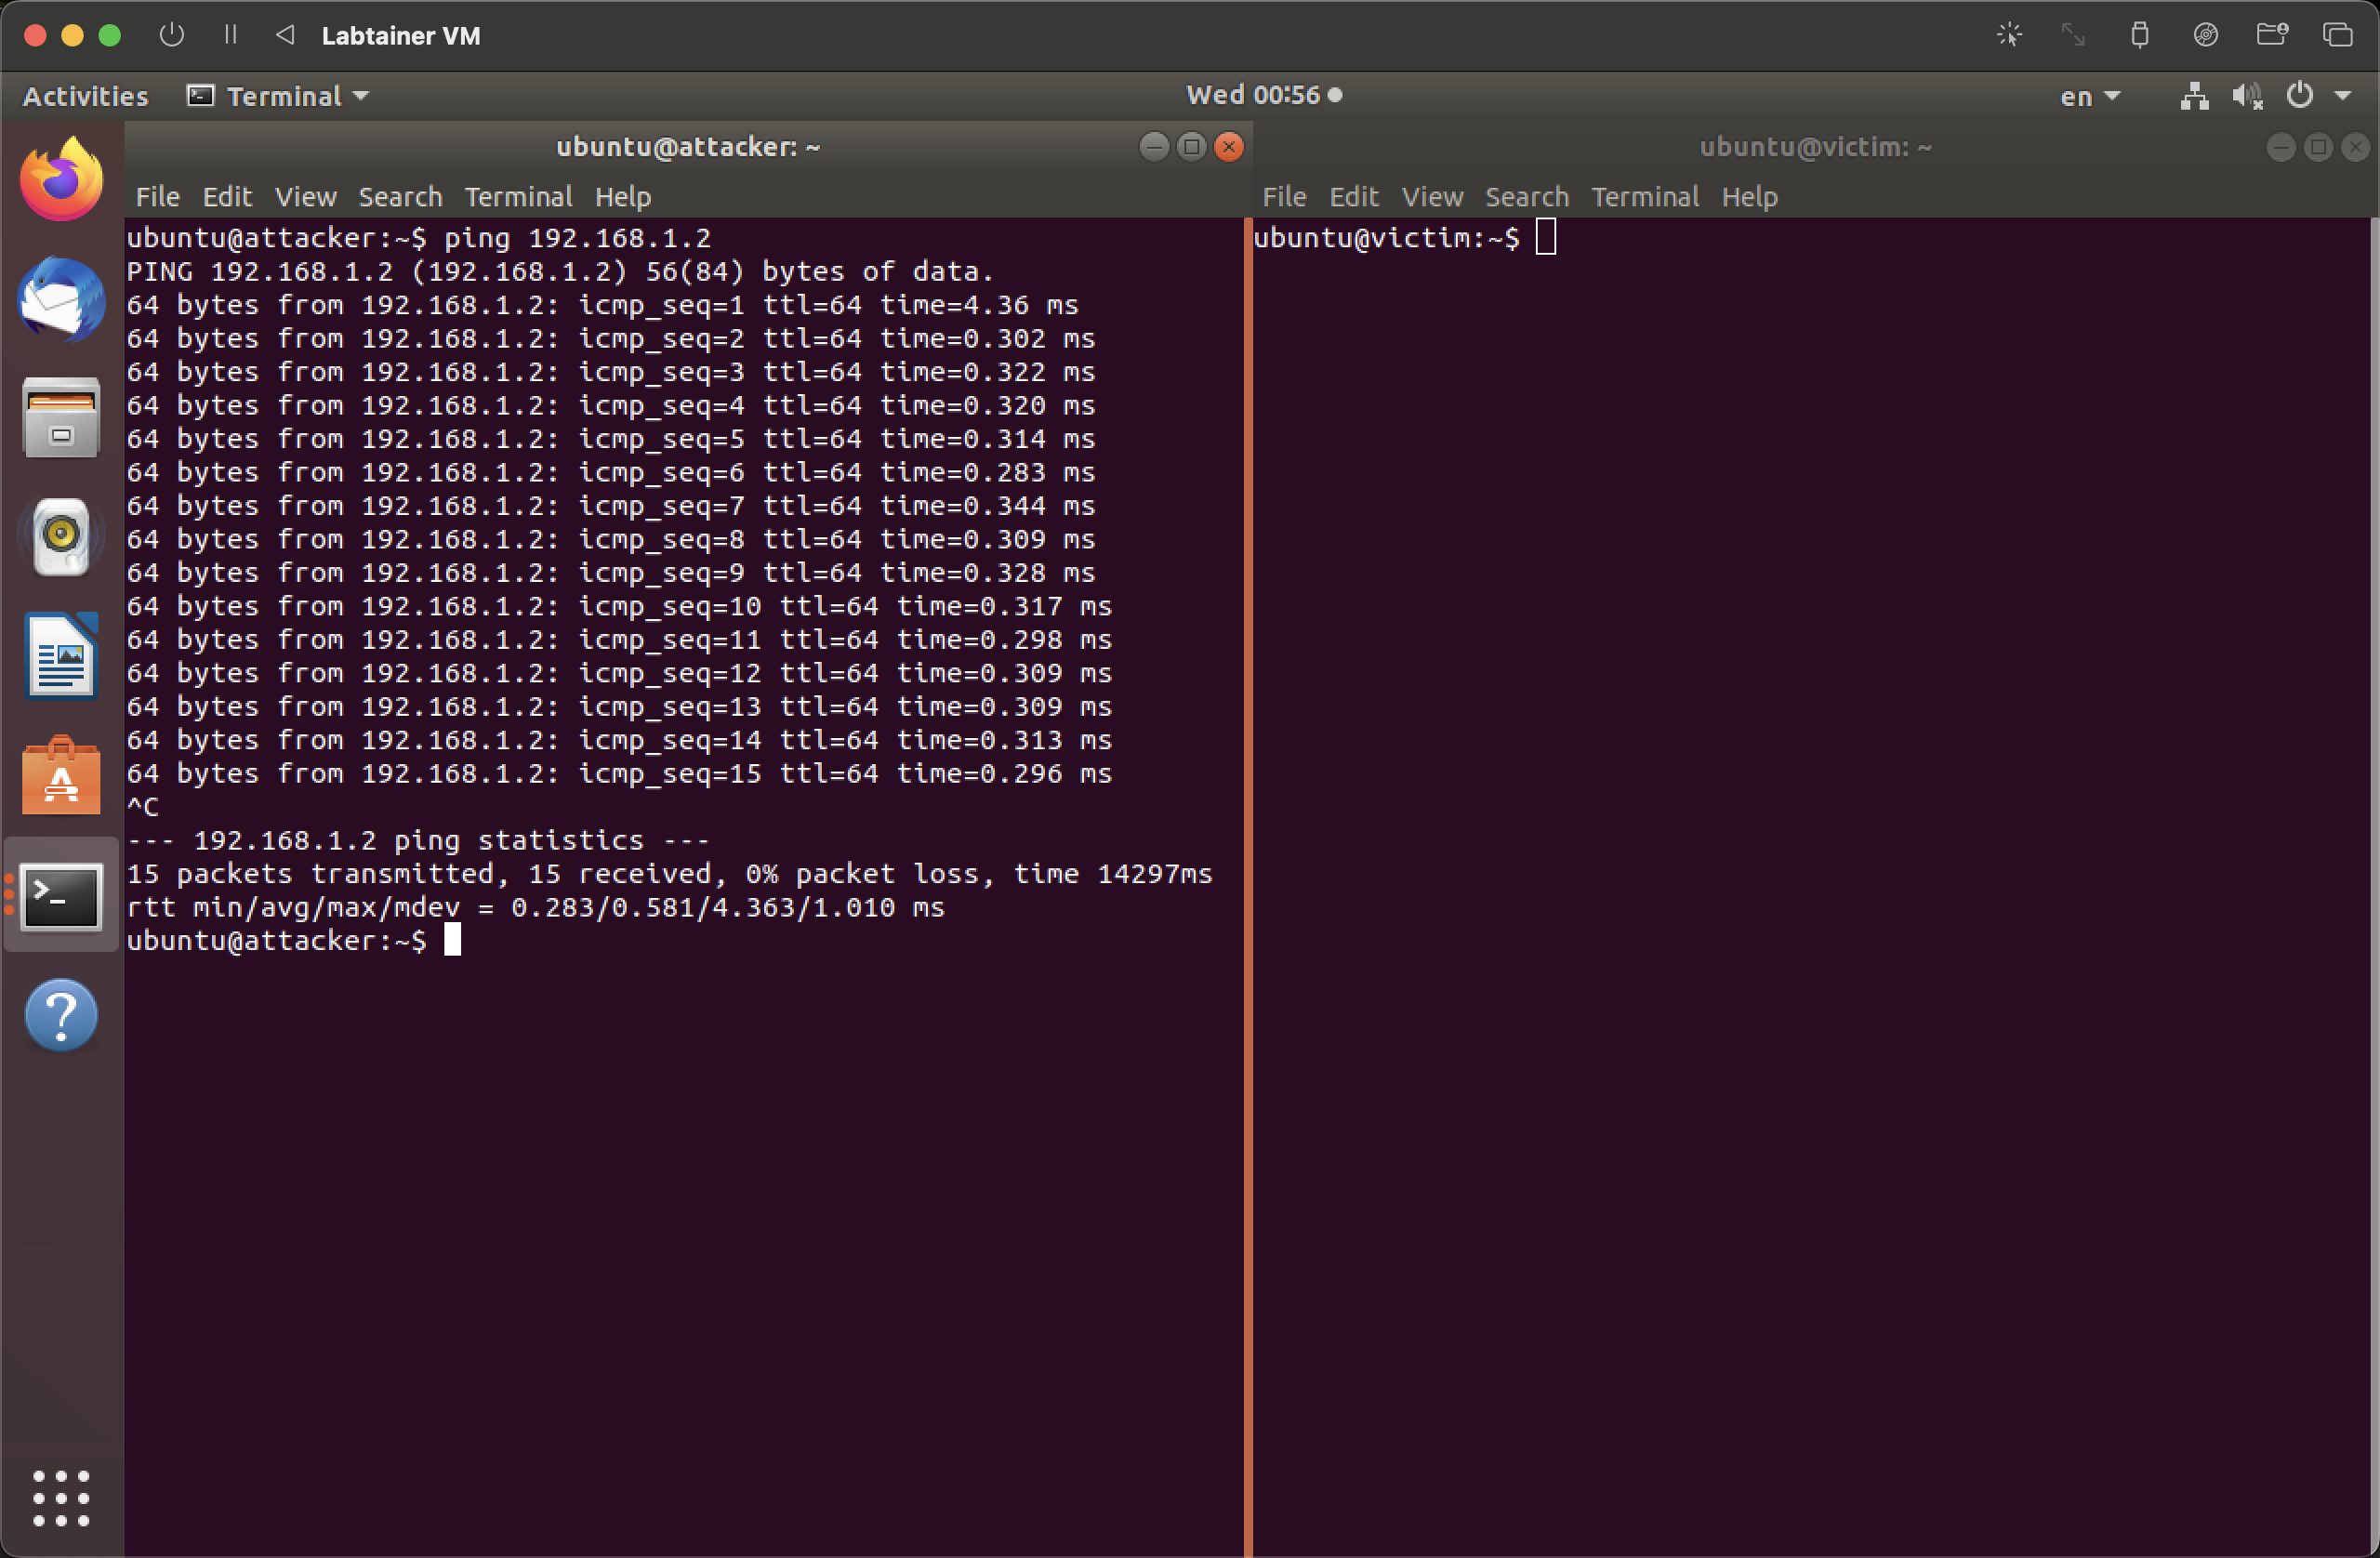
\includegraphics[width=0.7\textwidth]{images/02.png}
    \caption{Connection Check}
\end{figure}

\subsection{List of Vulnerable Services}
To find a list of the vulnerable services on the victims machine, we can use simply:
\[\texttt{nmap -p0-65535 192.168.1.2}\]

\begin{figure}[h!]
    \centering
    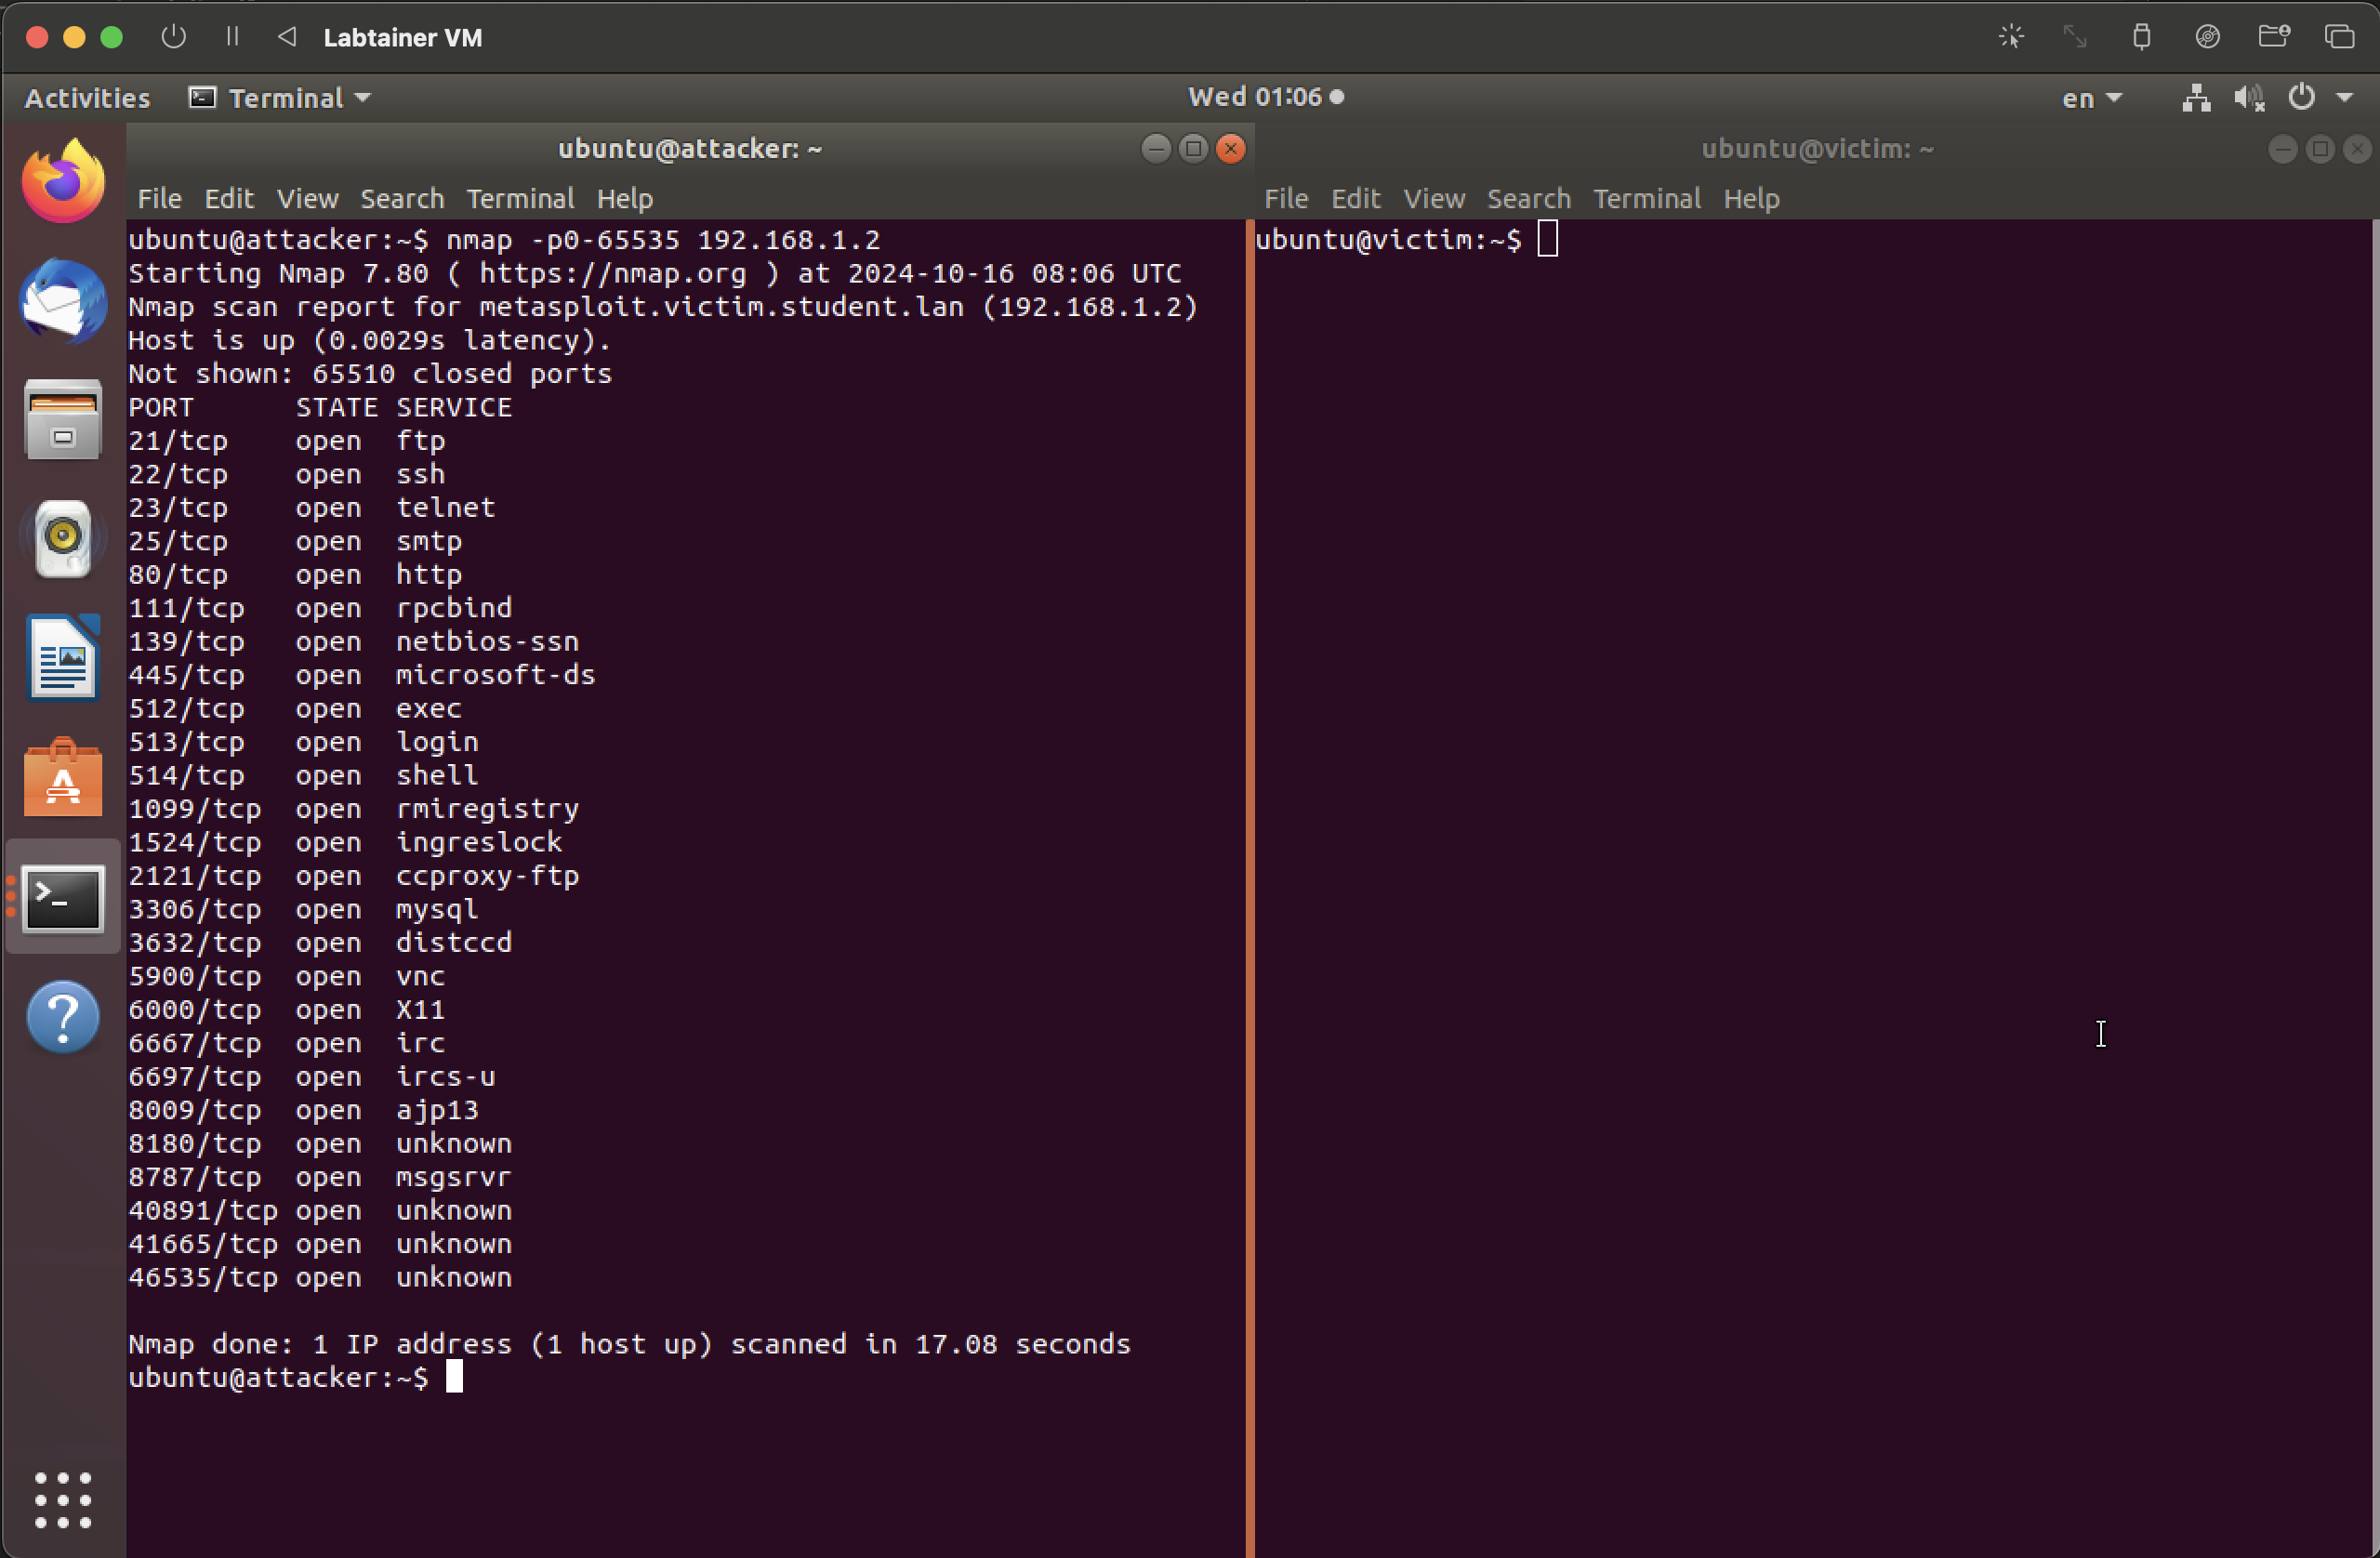
\includegraphics[width=0.7\textwidth]{images/03.png}
    \caption{List of Vulnerabilities}
\end{figure}

\subsection{Vulnerably Login Test}
In this part, we're going to login and test the connectivity to the victim machine executing a simple command, to check if we can read a file:
\[\texttt{rlogin -l root 192.168.1.2}\]

\begin{figure}[h!]
    \centering
    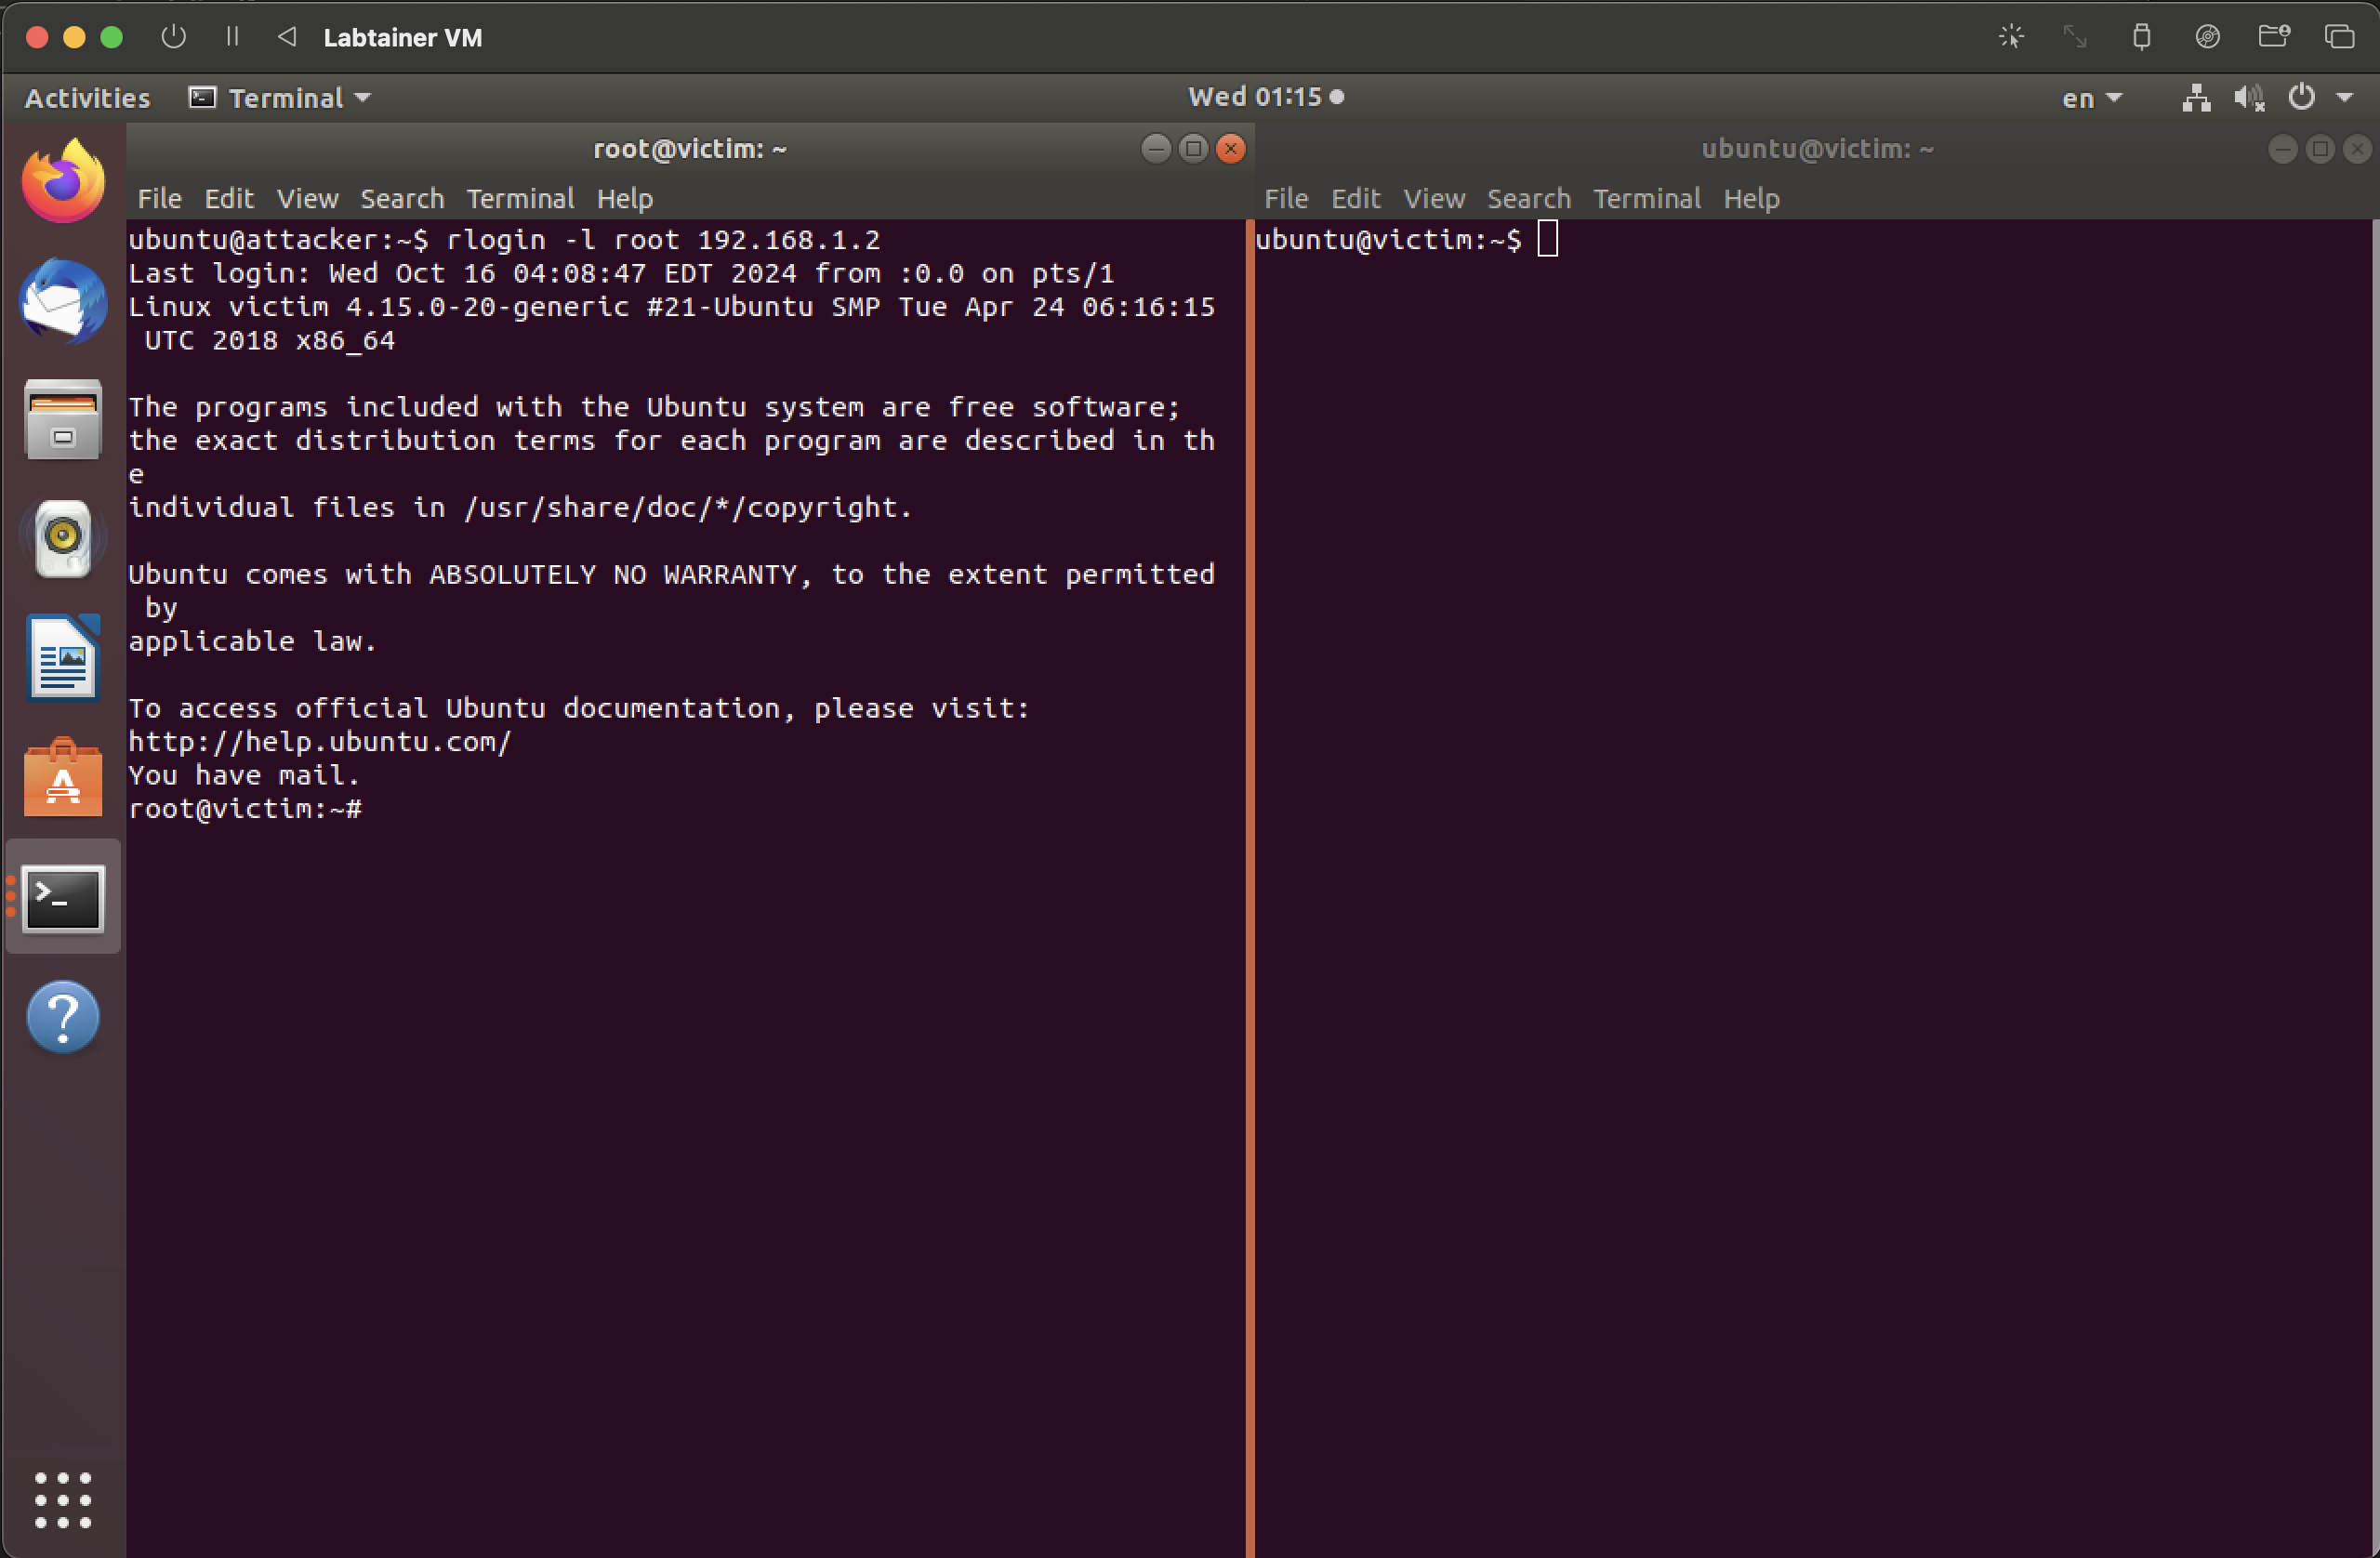
\includegraphics[width=0.7\textwidth]{images/04.png}
    \caption{Connectivity Test}
\end{figure}

and, to display the files:
\[\texttt{cat /root/filetoview.txt}\]

\begin{figure}[h!]
    \centering
    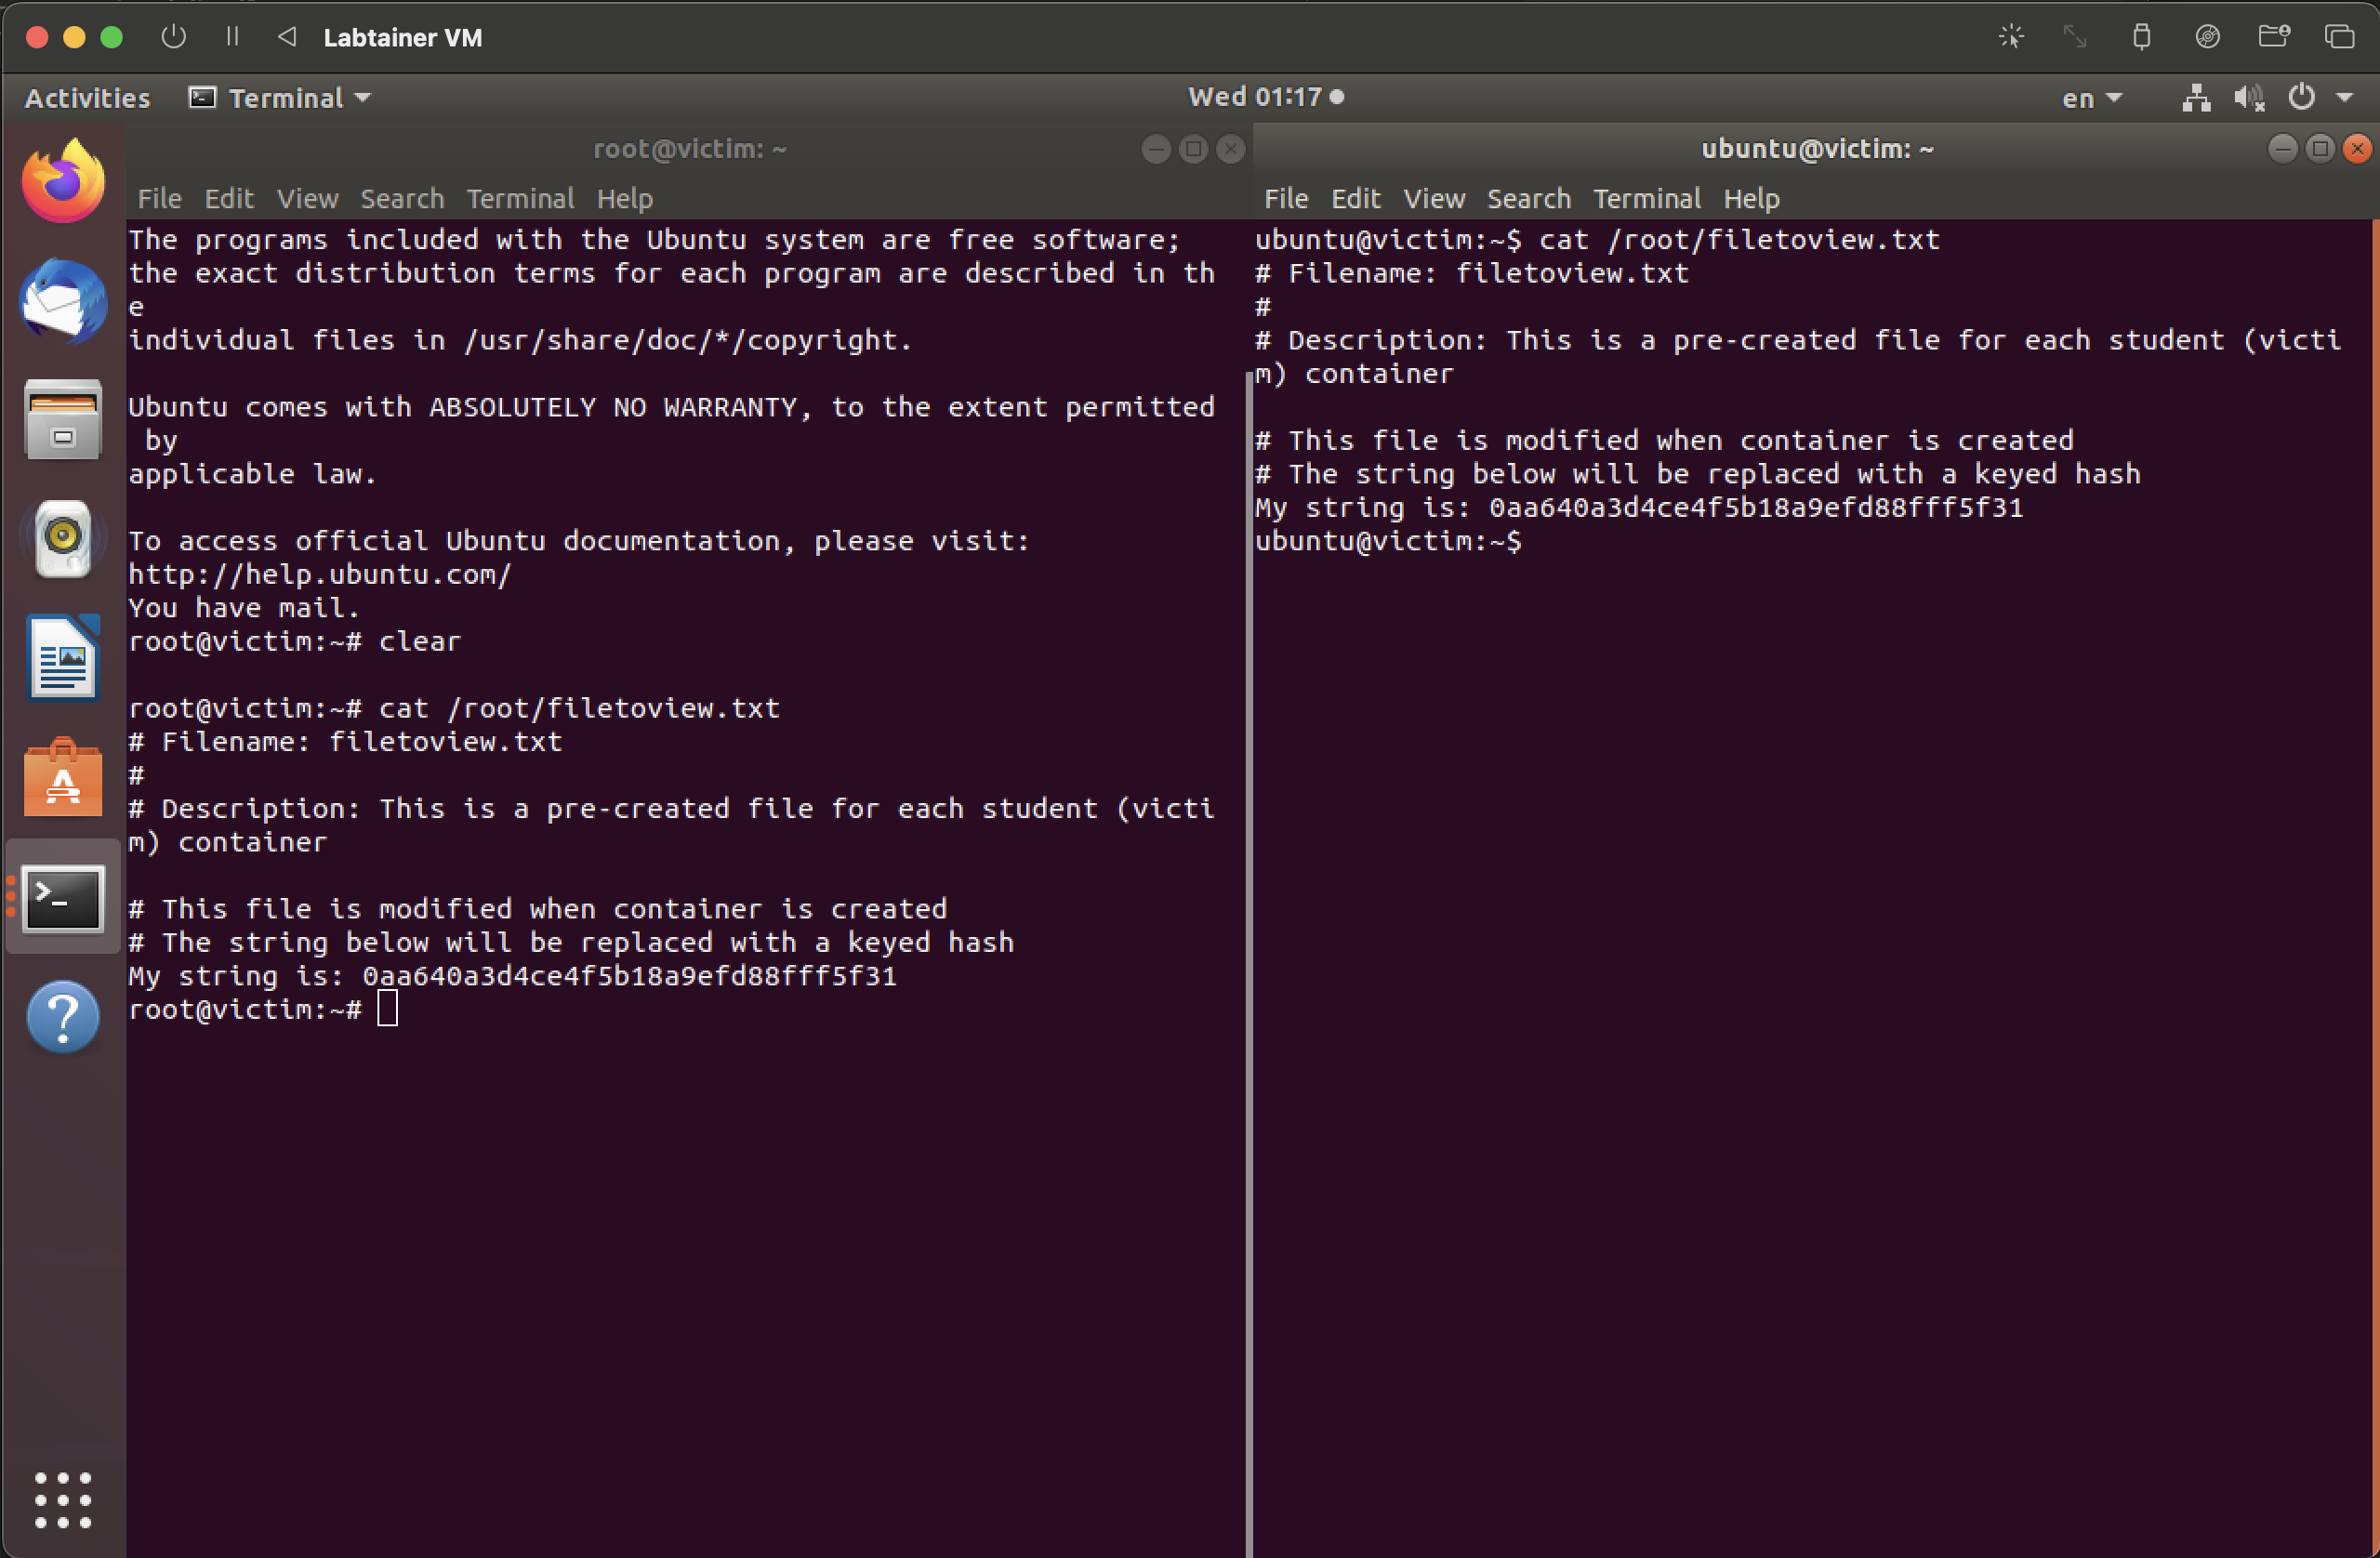
\includegraphics[width=0.7\textwidth]{images/05.png}
    \caption{File Test}
\end{figure}

\subsection{Exploit Tests}
In this part, we're going to test several exploits in the victims machine, each one, we're going to display a \texttt{root file}.

\subsubsection{Ingreslock Service (port 1524)}
Running \texttt{telnet 192.168.1.2 1524} tries to connect to port \texttt{1524} on the target machine. If there’s a backdoor service running on this port, it may grant direct access to the system without needing a password, simulating how attackers could exploit open or unsecured ports to gain unauthorized entry. This shows the importance of securing network services to prevent vulnerabilities.

\begin{figure}[h!]
    \centering
    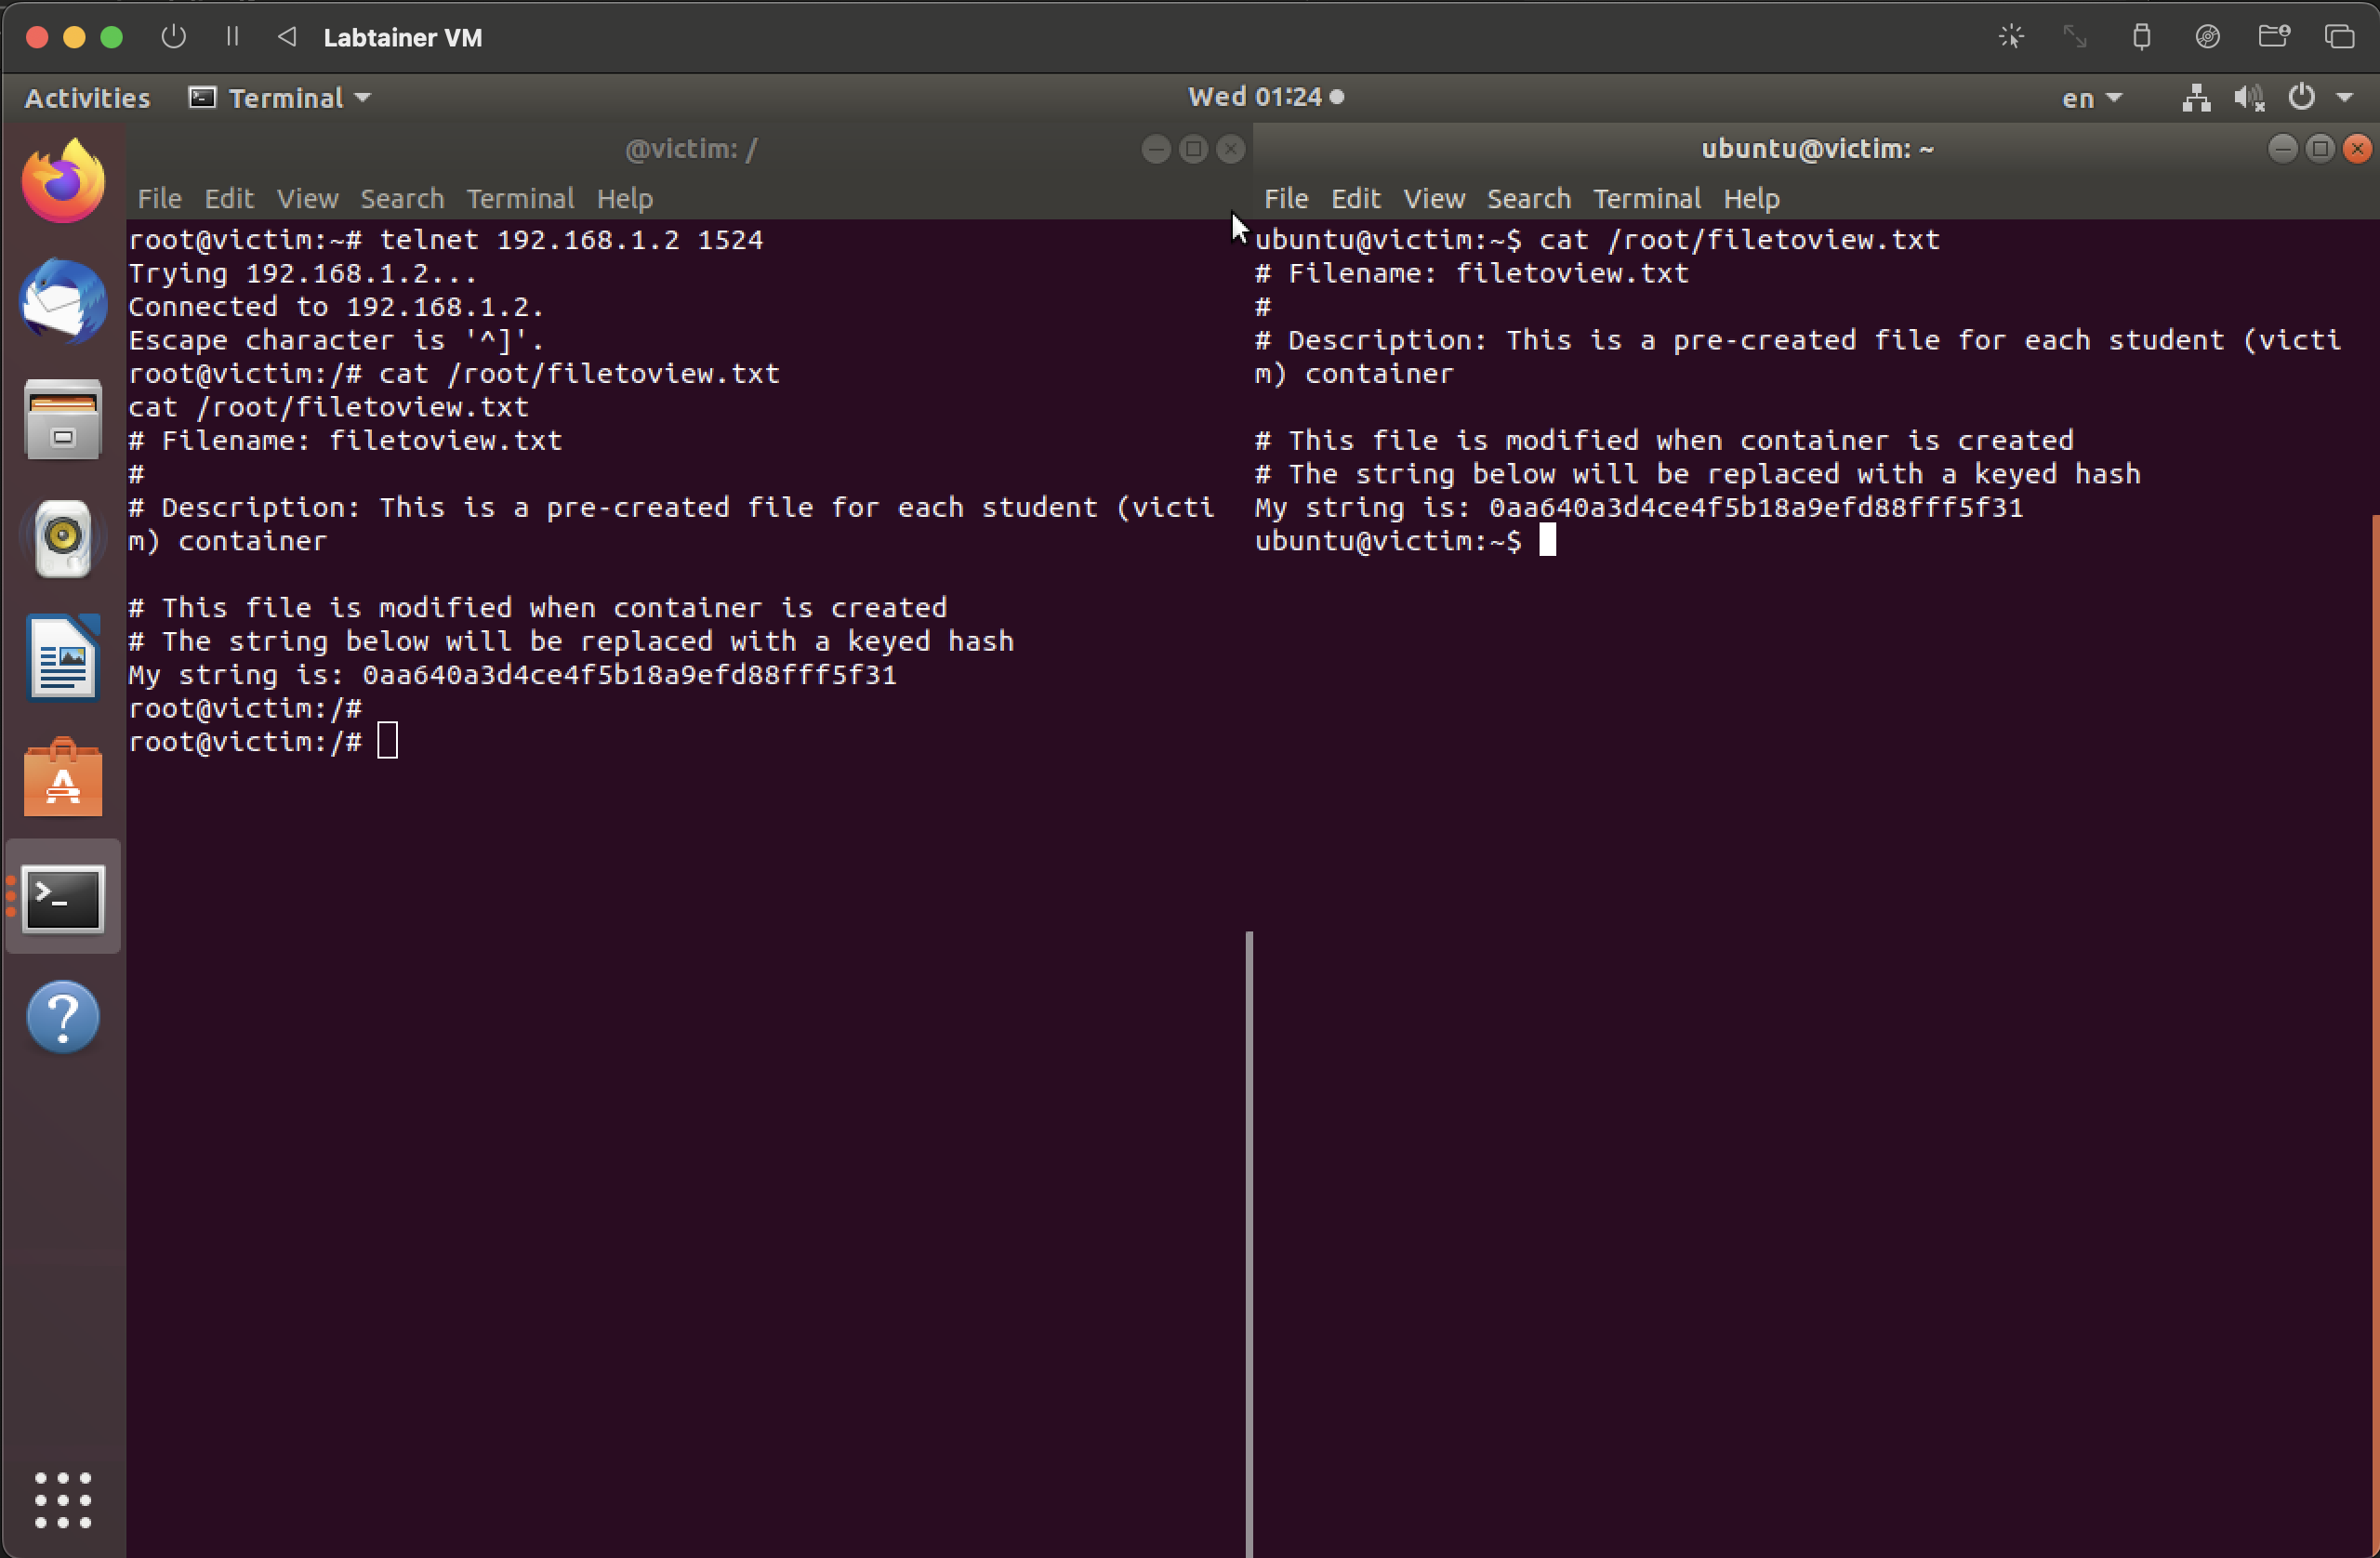
\includegraphics[width=0.7\textwidth]{images/06.png}
    \caption{Ingreslock Test}
\end{figure}

\subsubsection{Distccd service (port 3632)}
The distccd service is a tool designed for distributed compilation, allowing multiple computers to work together to speed up the software build process. By running distccd on a server, client machines can send compilation tasks over the network, and the server performs these tasks and returns the results, significantly reducing build times. Distccd typically listens on port 3632. However, earlier versions of distccd had security issues because they lacked proper authentication, allowing any machine on the network to connect and execute commands. This vulnerability led to the creation of specific exploits, such as the one in Metasploit (exploit/unix/misc/distcc\_exec), which allows attackers to gain unauthorized access by executing commands on vulnerable servers. To prevent exploitation, distccd should be properly secured, restricting access to trusted machines only and ensuring it is not exposed to untrusted networks.

\begin{figure}[h!]
    \centering
    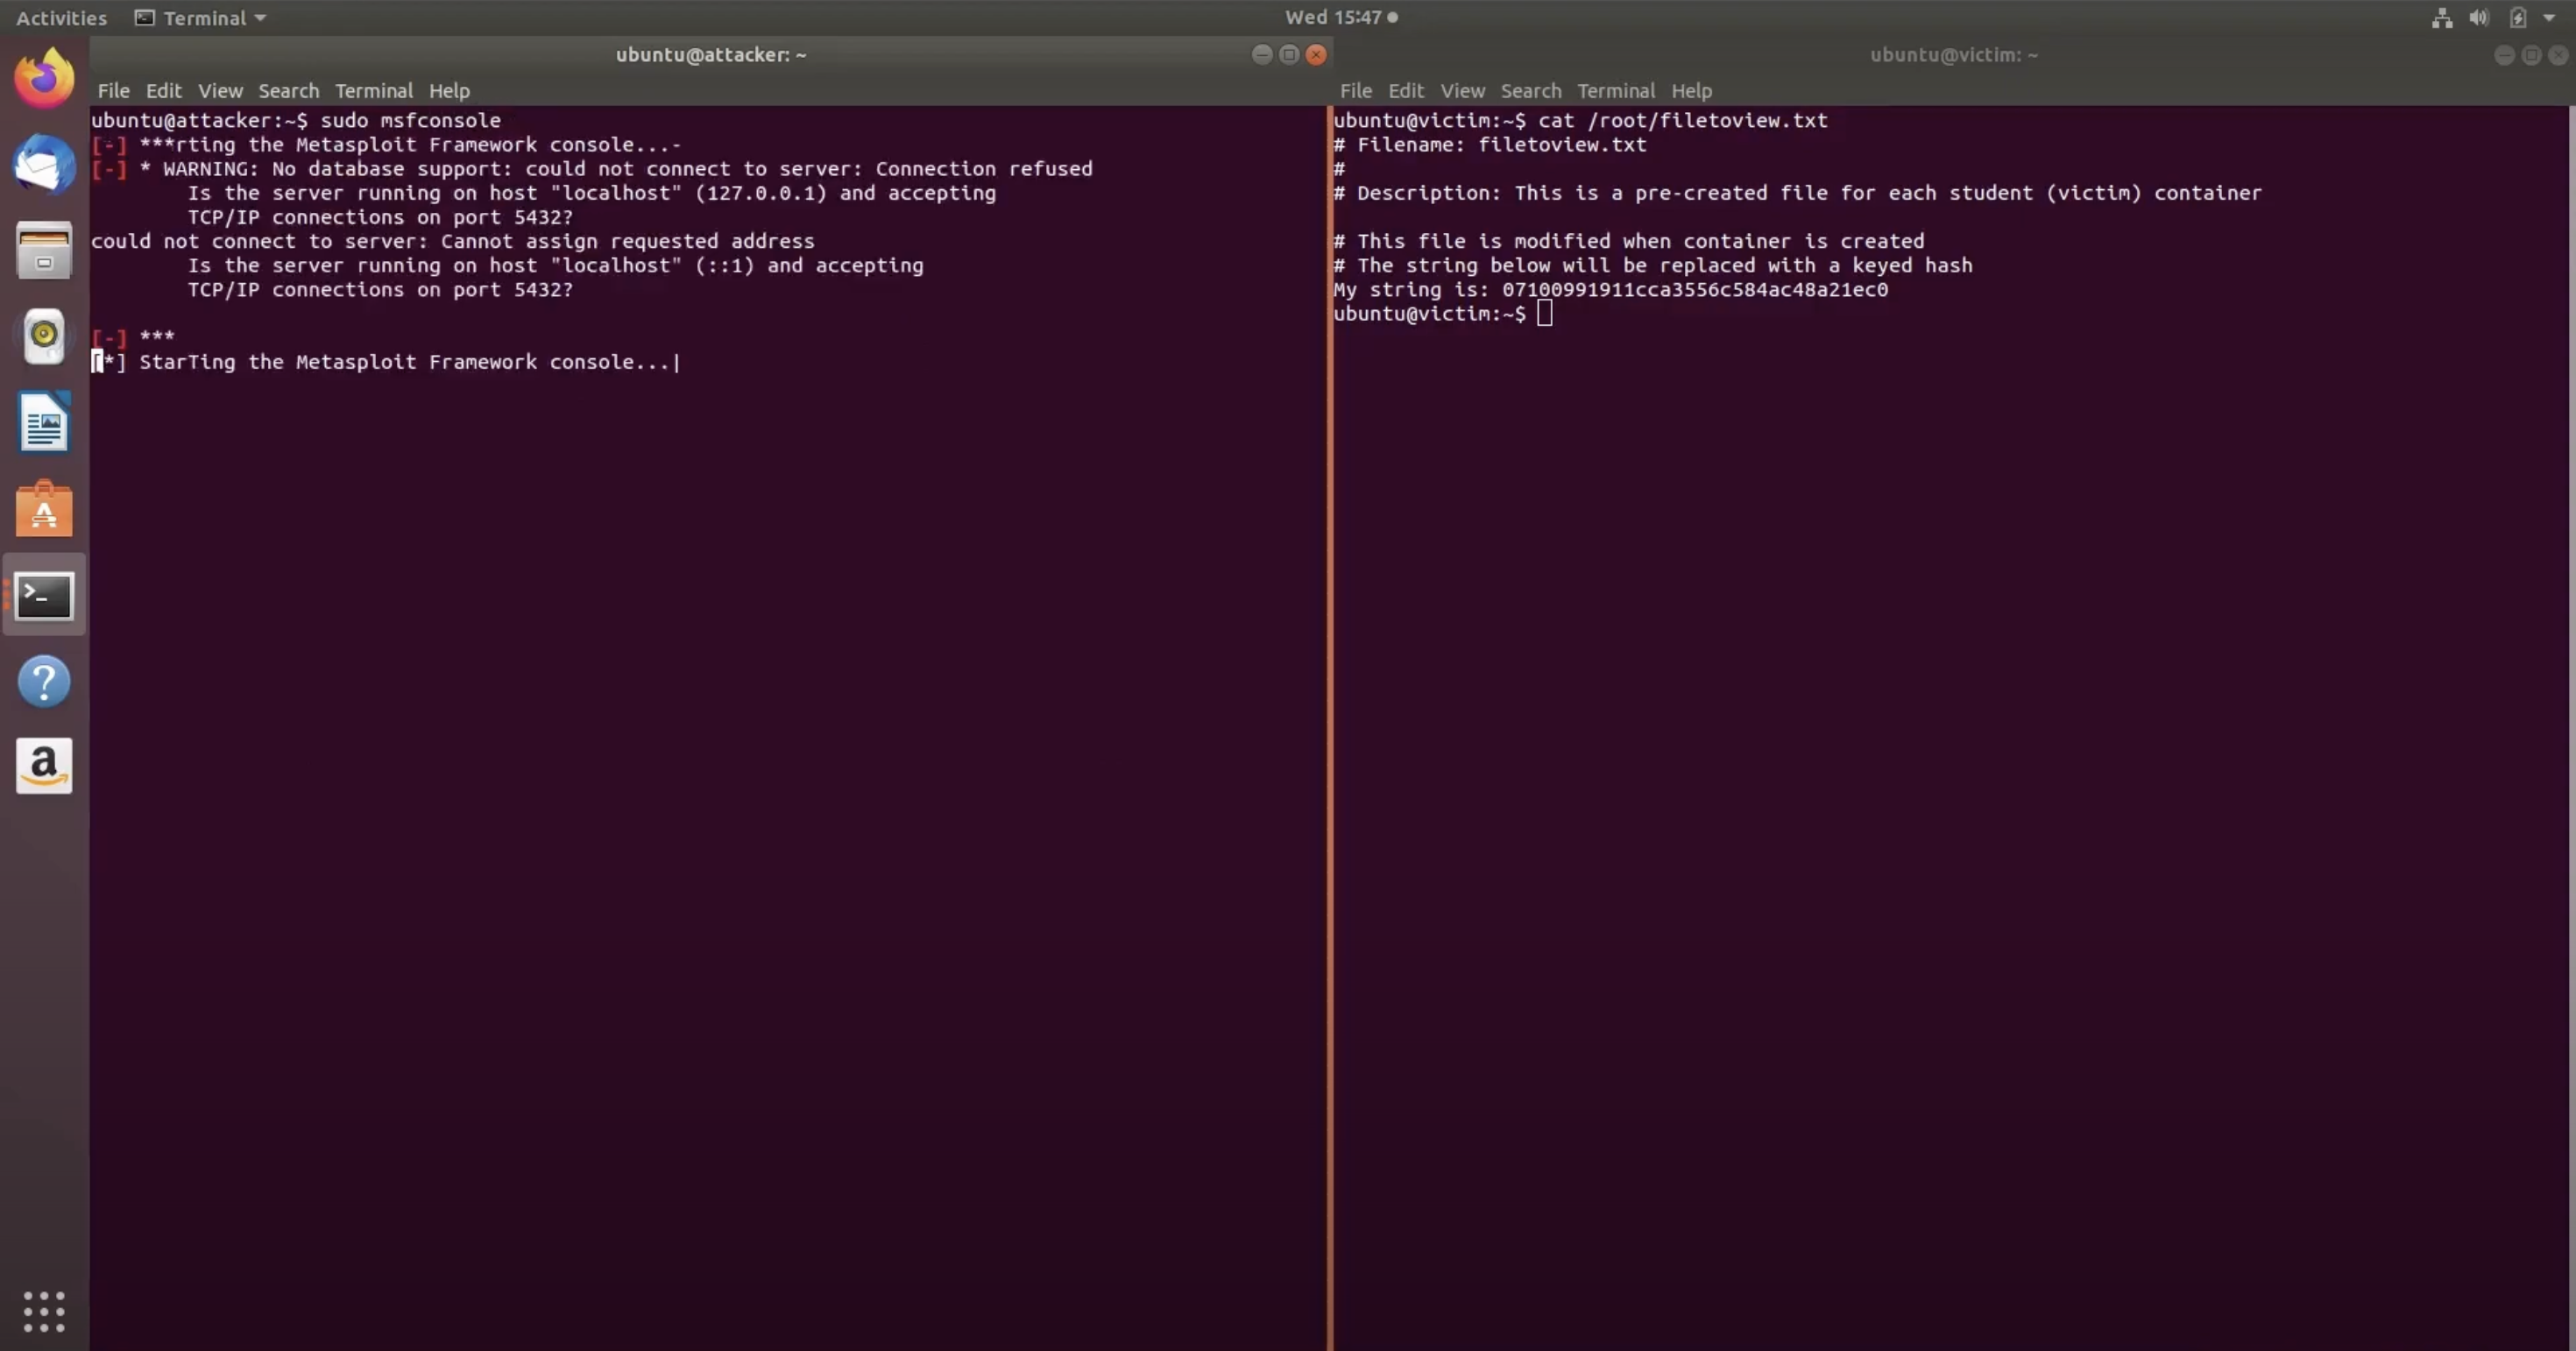
\includegraphics[width=0.7\textwidth]{images/07.png}
    \caption{\texttt{msfconsole}}
\end{figure}

\break

\begin{figure}[h!]
    \centering
    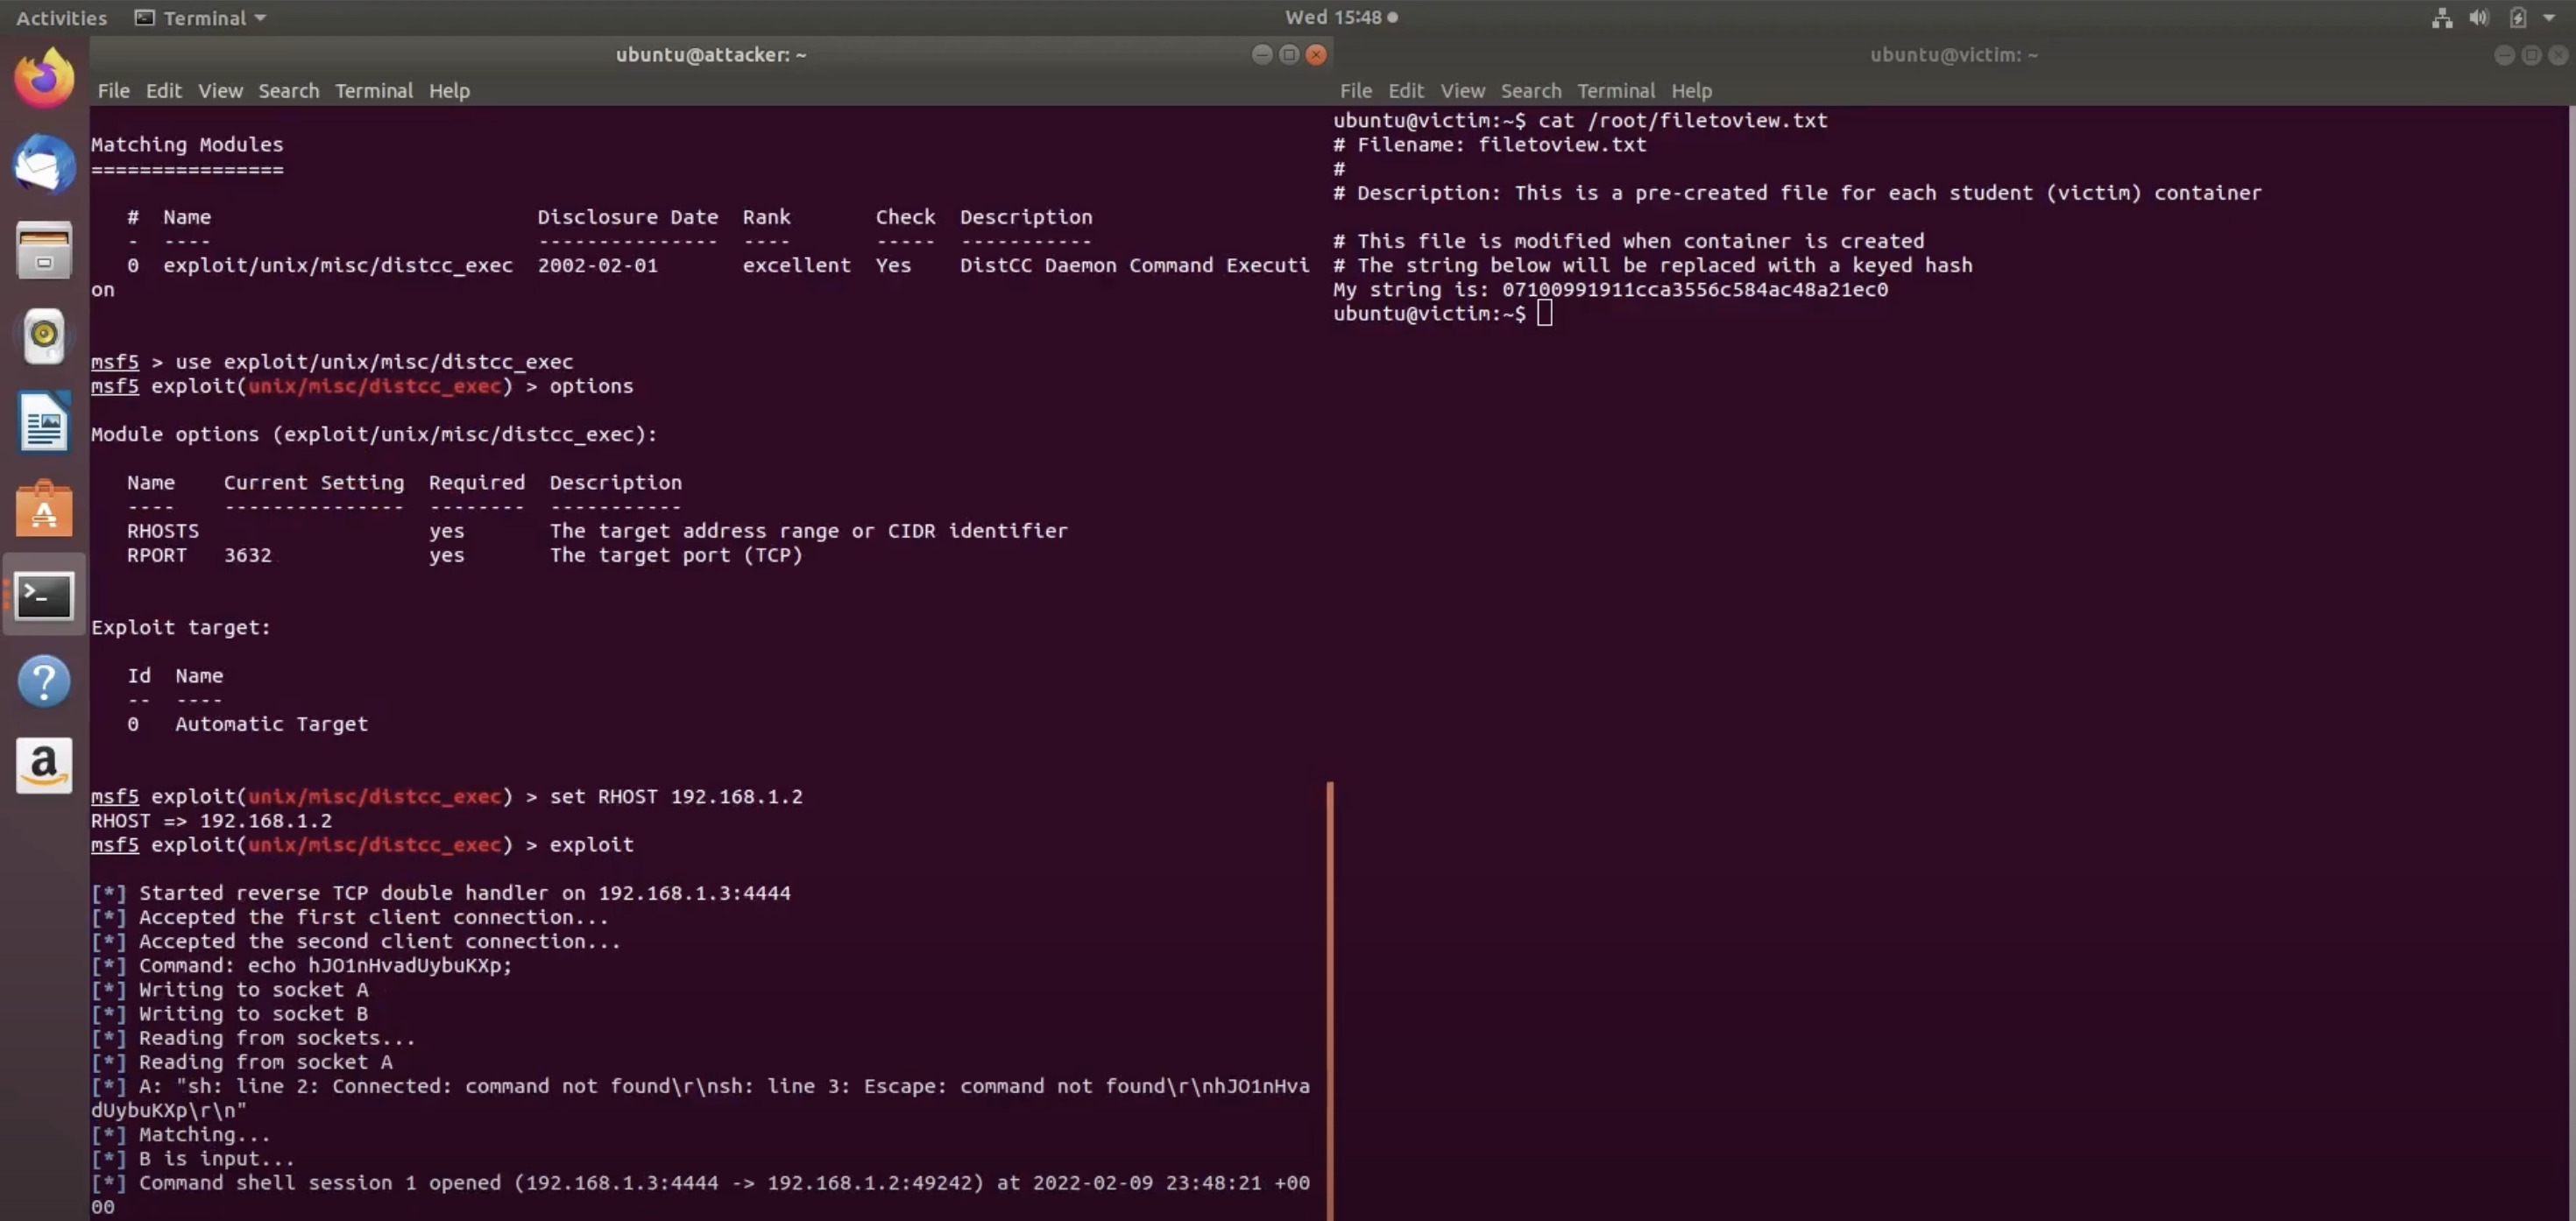
\includegraphics[width=0.7\textwidth]{images/08.png}
    \caption{Exploit}
    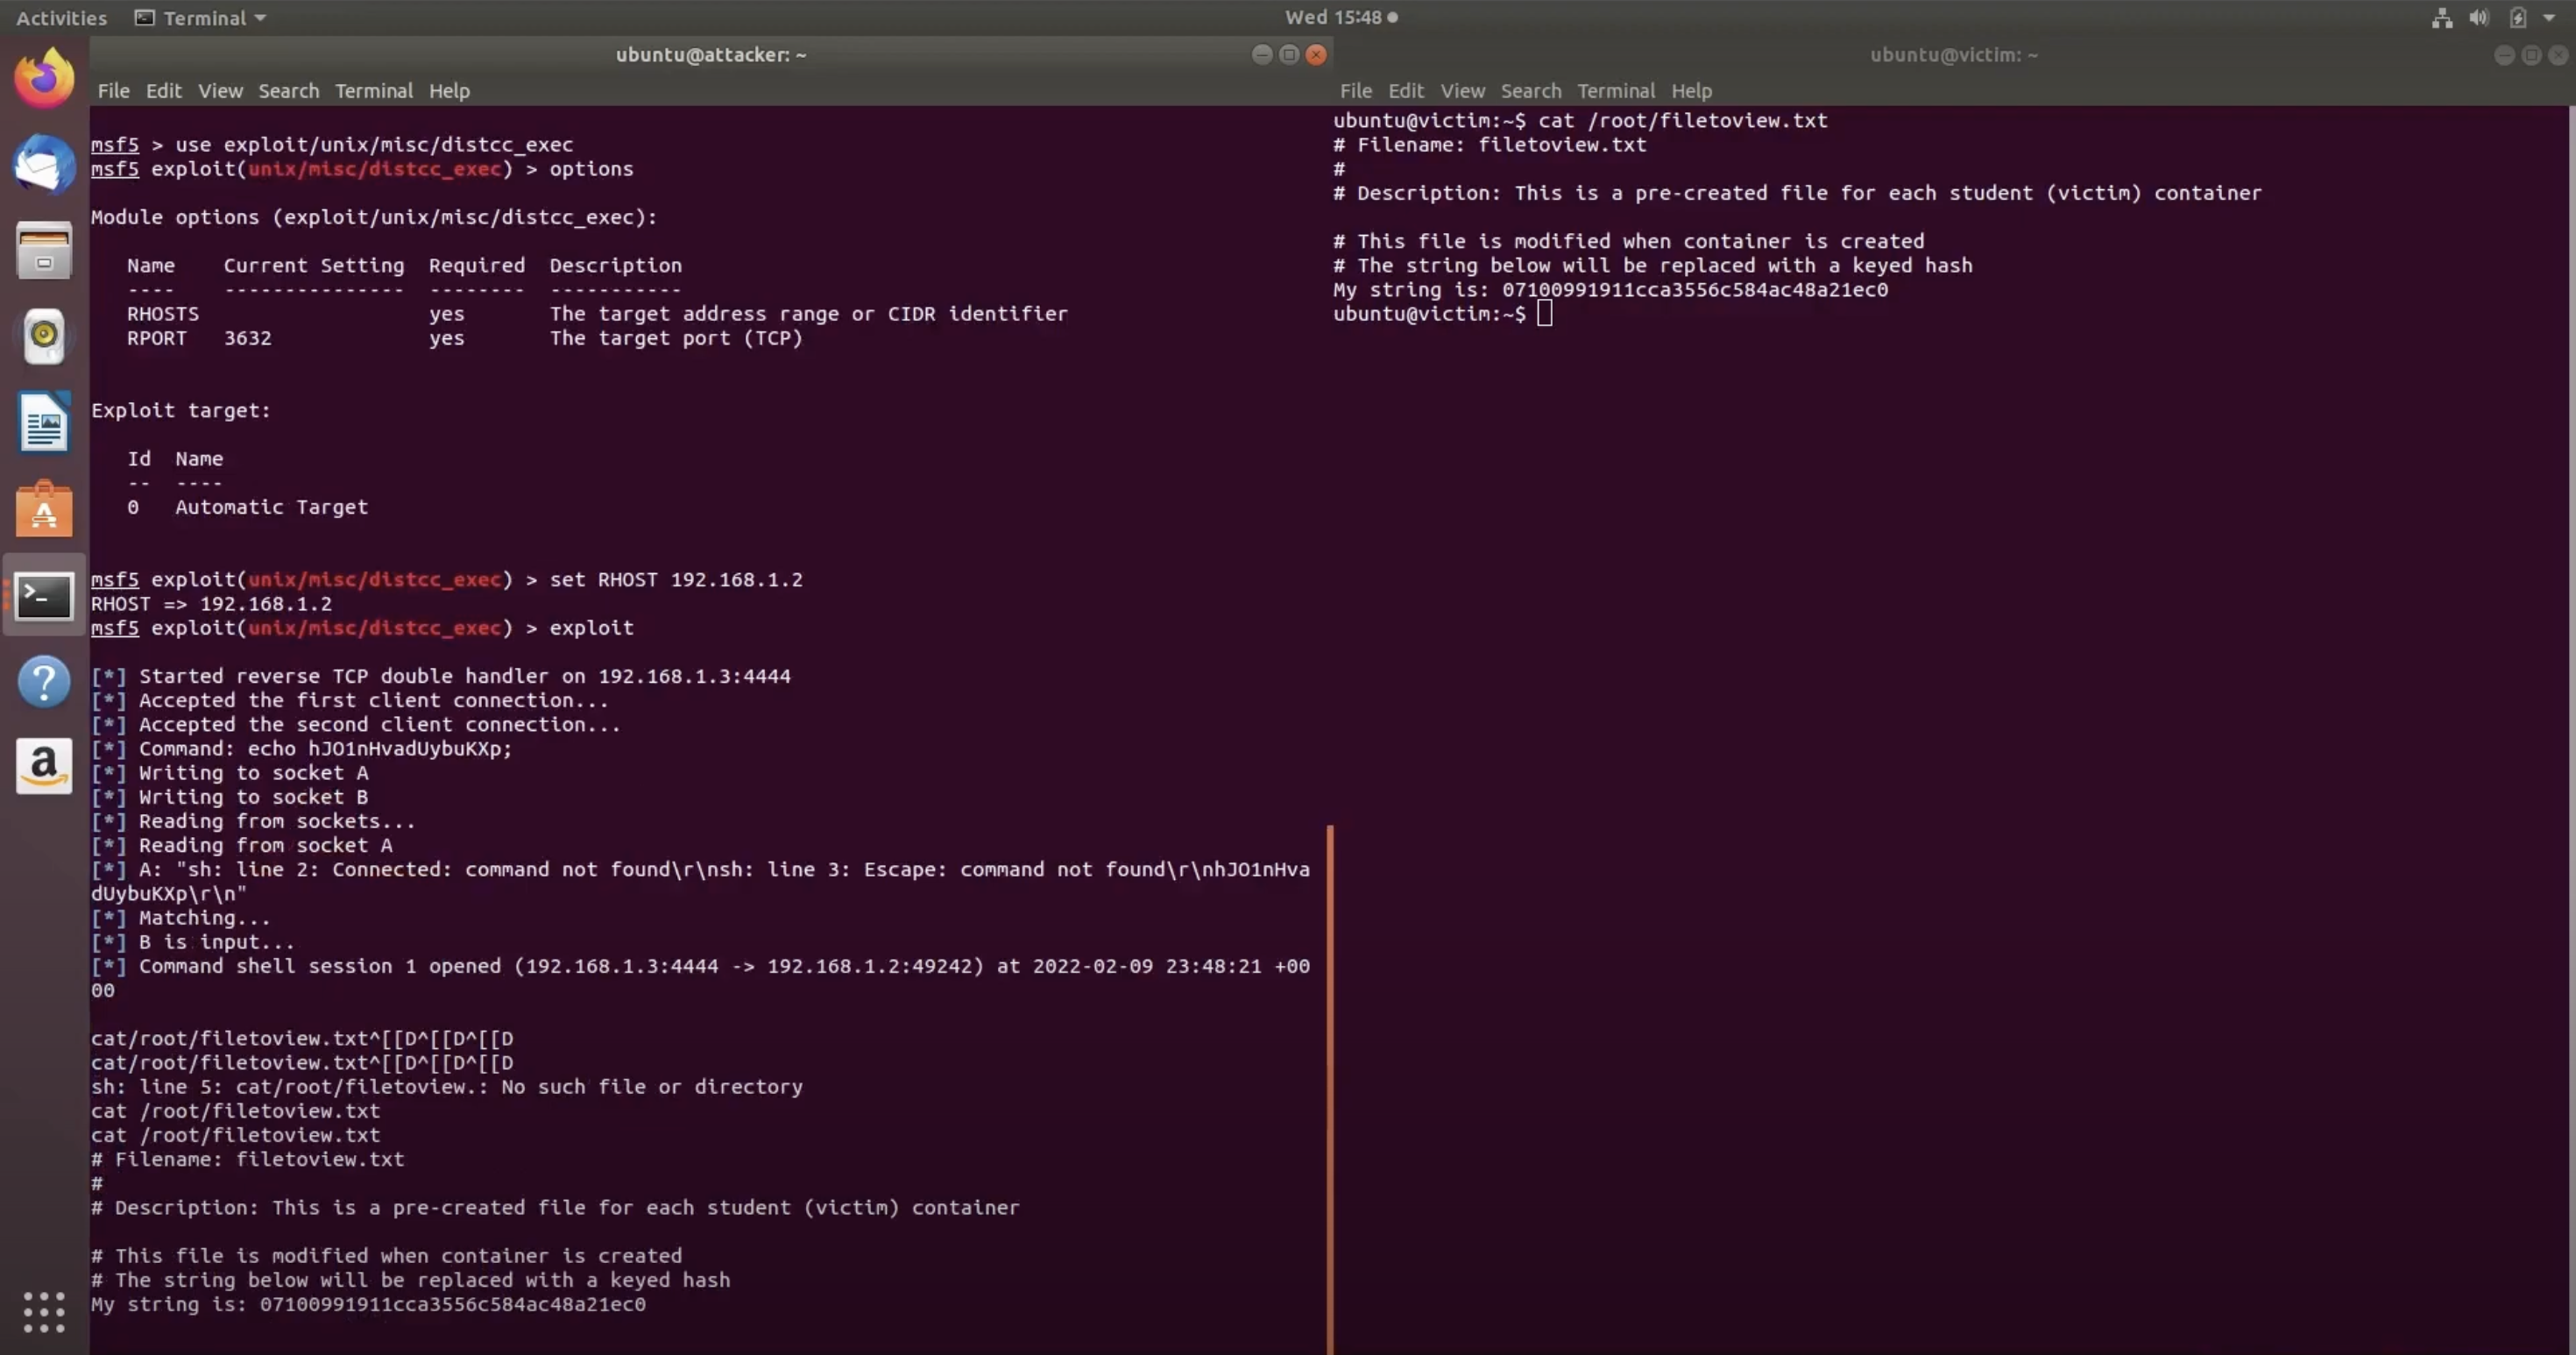
\includegraphics[width=0.7\textwidth]{images/09.png}
    \caption{Root Test}
\end{figure}

\subsubsection{IRC daemon (port 6667)}
UnrealIRCd is an open-source IRC daemon that enables the creation of chat servers. Between November 2009 and June 2010, a compromised version of UnrealIRCd 3.2.8.1 was distributed, containing a backdoor that allowed remote command execution on the server. This vulnerability is cataloged under CVE-2010-2075.\\
To exploit this vulnerability using Metasploit, start by launching the Metasploit console with sudo msfconsole. Then, search for the exploit with search unreal\_ircd and select the appropriate exploit with use exploit/unix/irc/unreal\_ircd\_3281\_backdoor. To view the available options, use show options. Next, set the remote host (RHOST) IP address with set RHOST 192.168.1.2 and run the exploit with exploit. \\
After successful execution, a shell will be obtained on the vulnerable server, granting direct access. To confirm access, you can list the root directory contents with ls /. 

\break 

\begin{figure}[h!]
    \centering
    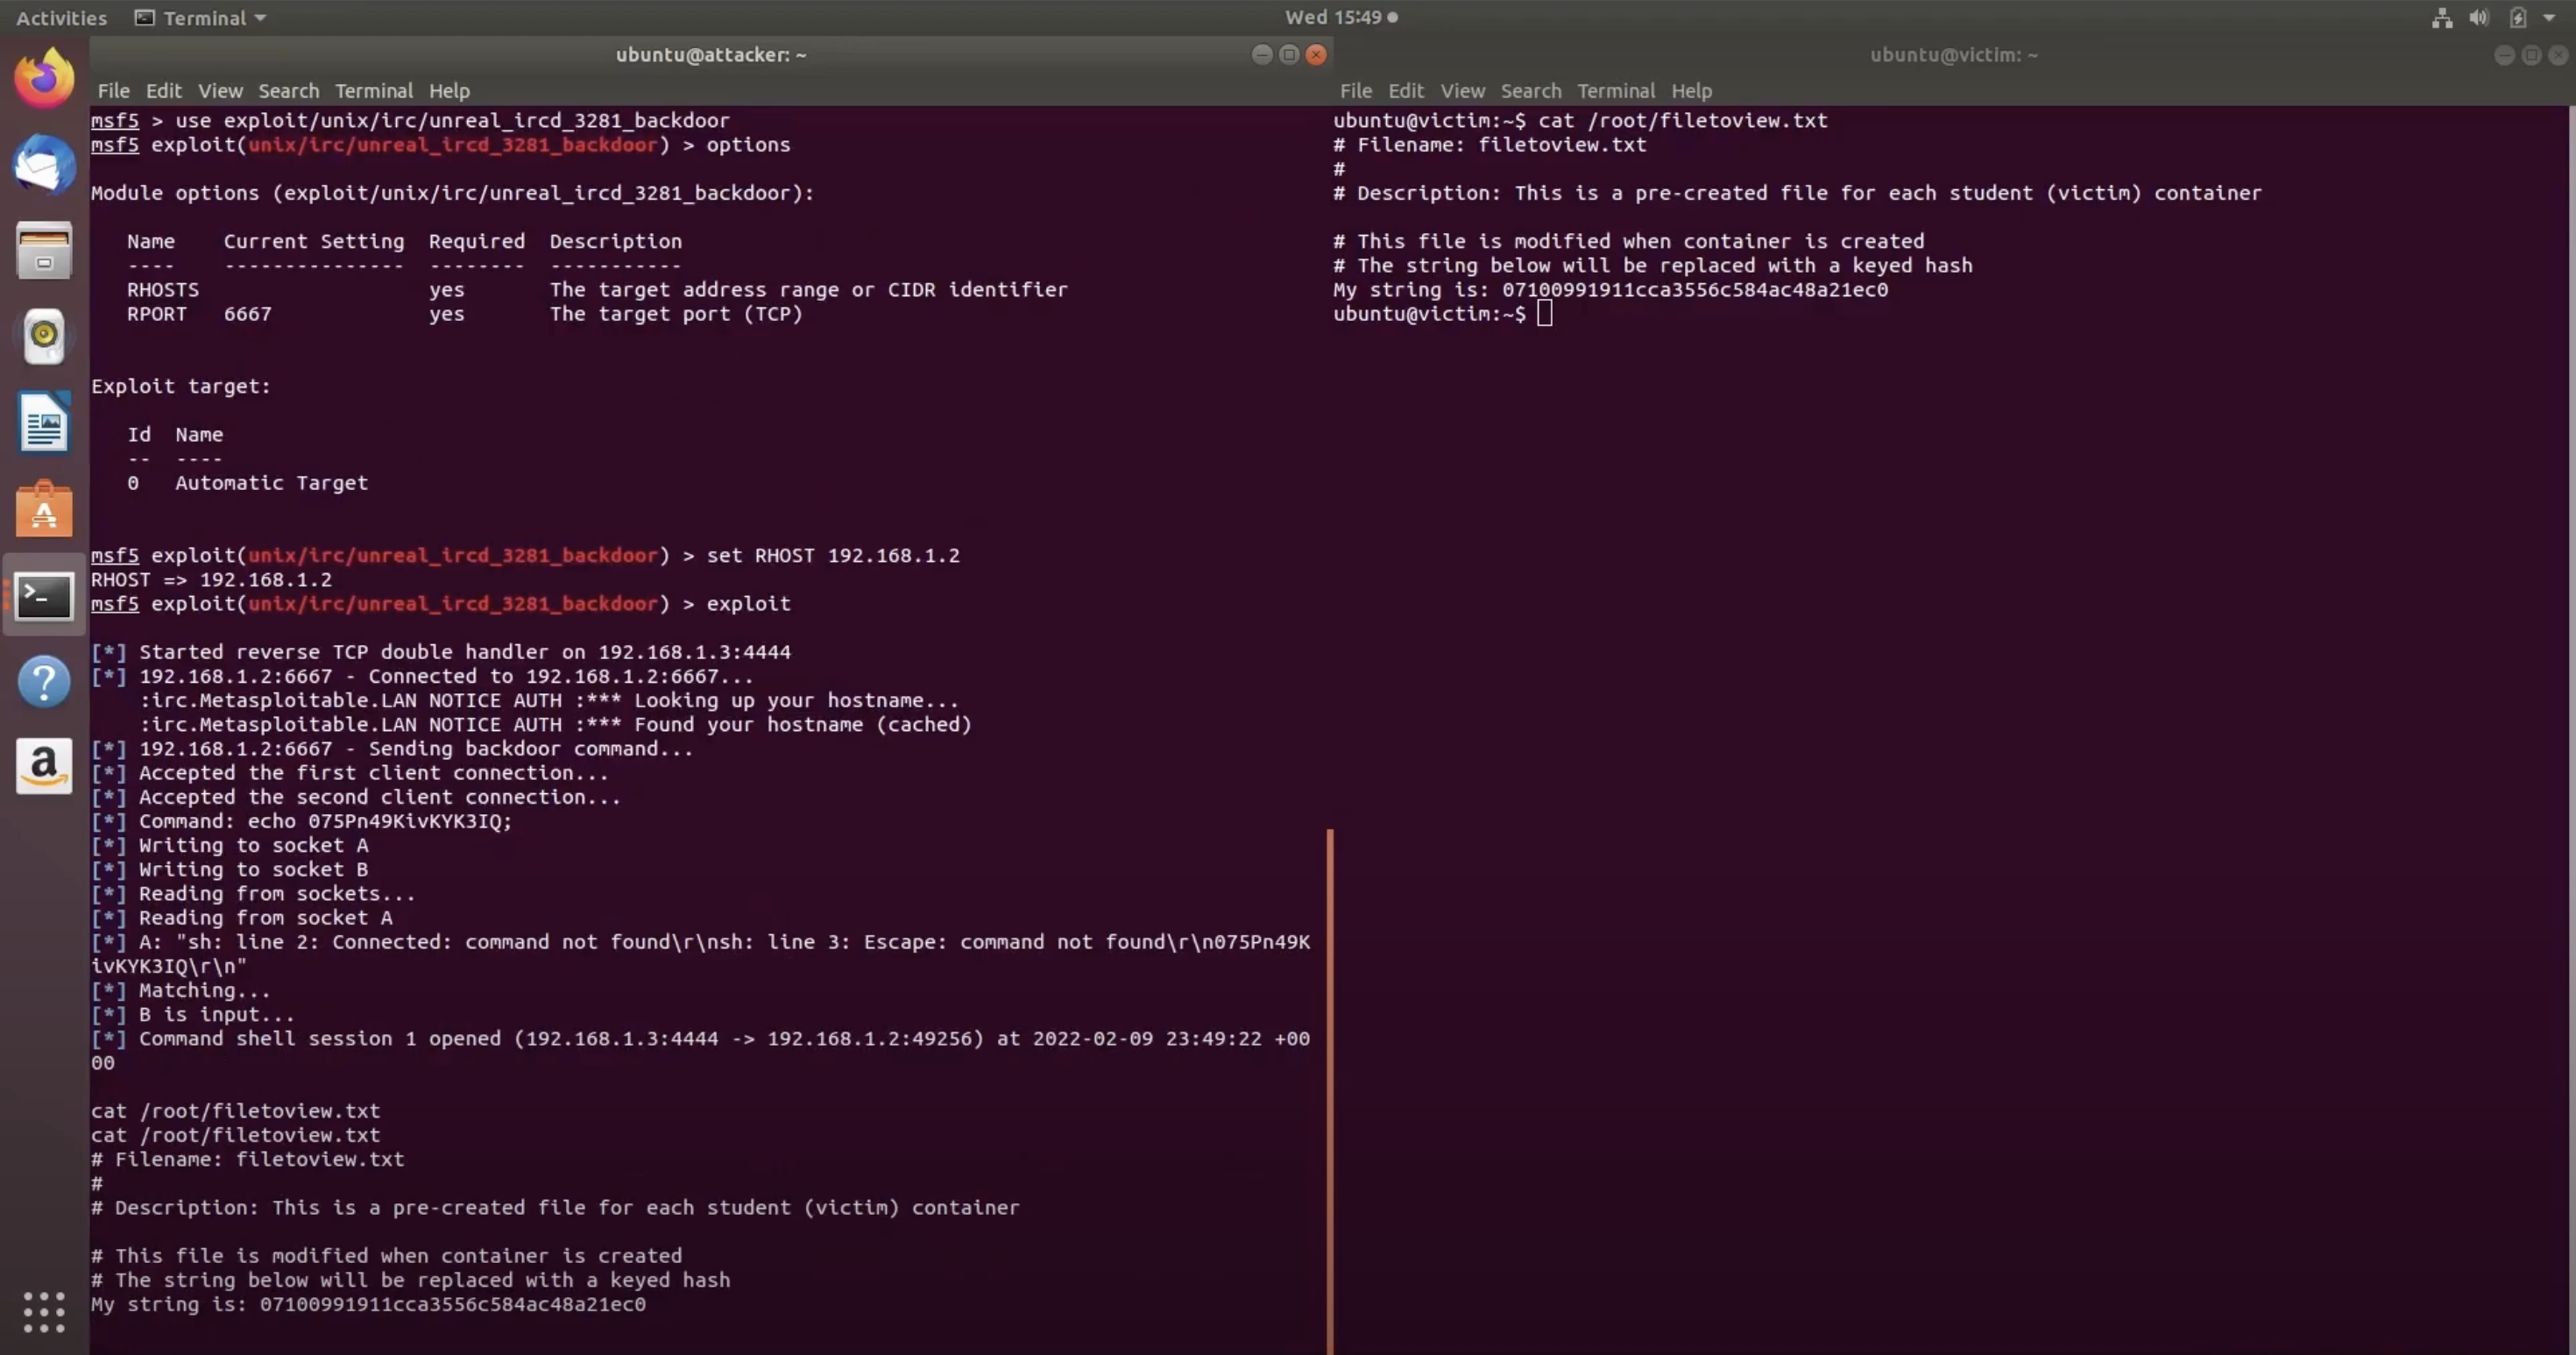
\includegraphics[width=0.7\textwidth]{images/10.png}
    \caption{IRC Daemon Test}
\end{figure}

\subsubsection{VSFtpd service (port 21)}
The VSFTPD (Very Secure FTP Daemon) service, typically running on port 21, is a popular FTP server software focused on security. However, in 2011, a backdoored version, VSFTPD 2.3.4, was briefly distributed, containing a hidden vulnerability that allowed attackers to exploit an unauthorized access backdoor. This vulnerability is cataloged as CVE-2011-2523.\\
In this lab, you will use Metasploit to exploit this vulnerability on a target server. The steps are as follows: First, start Metasploit and search for the vsftpd\_234 exploit using search vsftpd\_234. Then, load the exploit with use exploit/unix/ftp/vsftpd\_234\_backdoor. After that, view and configure the necessary options with show options, setting the target IP as the remote host (RHOST) using set RHOST 192.168.1.2. Finally, run the exploit with exploit.\\
Upon successful execution, a shell will be opened, allowing you to interact with the server. You can confirm access by listing the root directory contents with ls \/. This lab simulates how attackers could exploit the VSFTPD 2.3.4 backdoor to gain unauthorized shell access, demonstrating the importance of securing vulnerable services to prevent such exploits. 

\begin{figure}[h!]
    \centering
    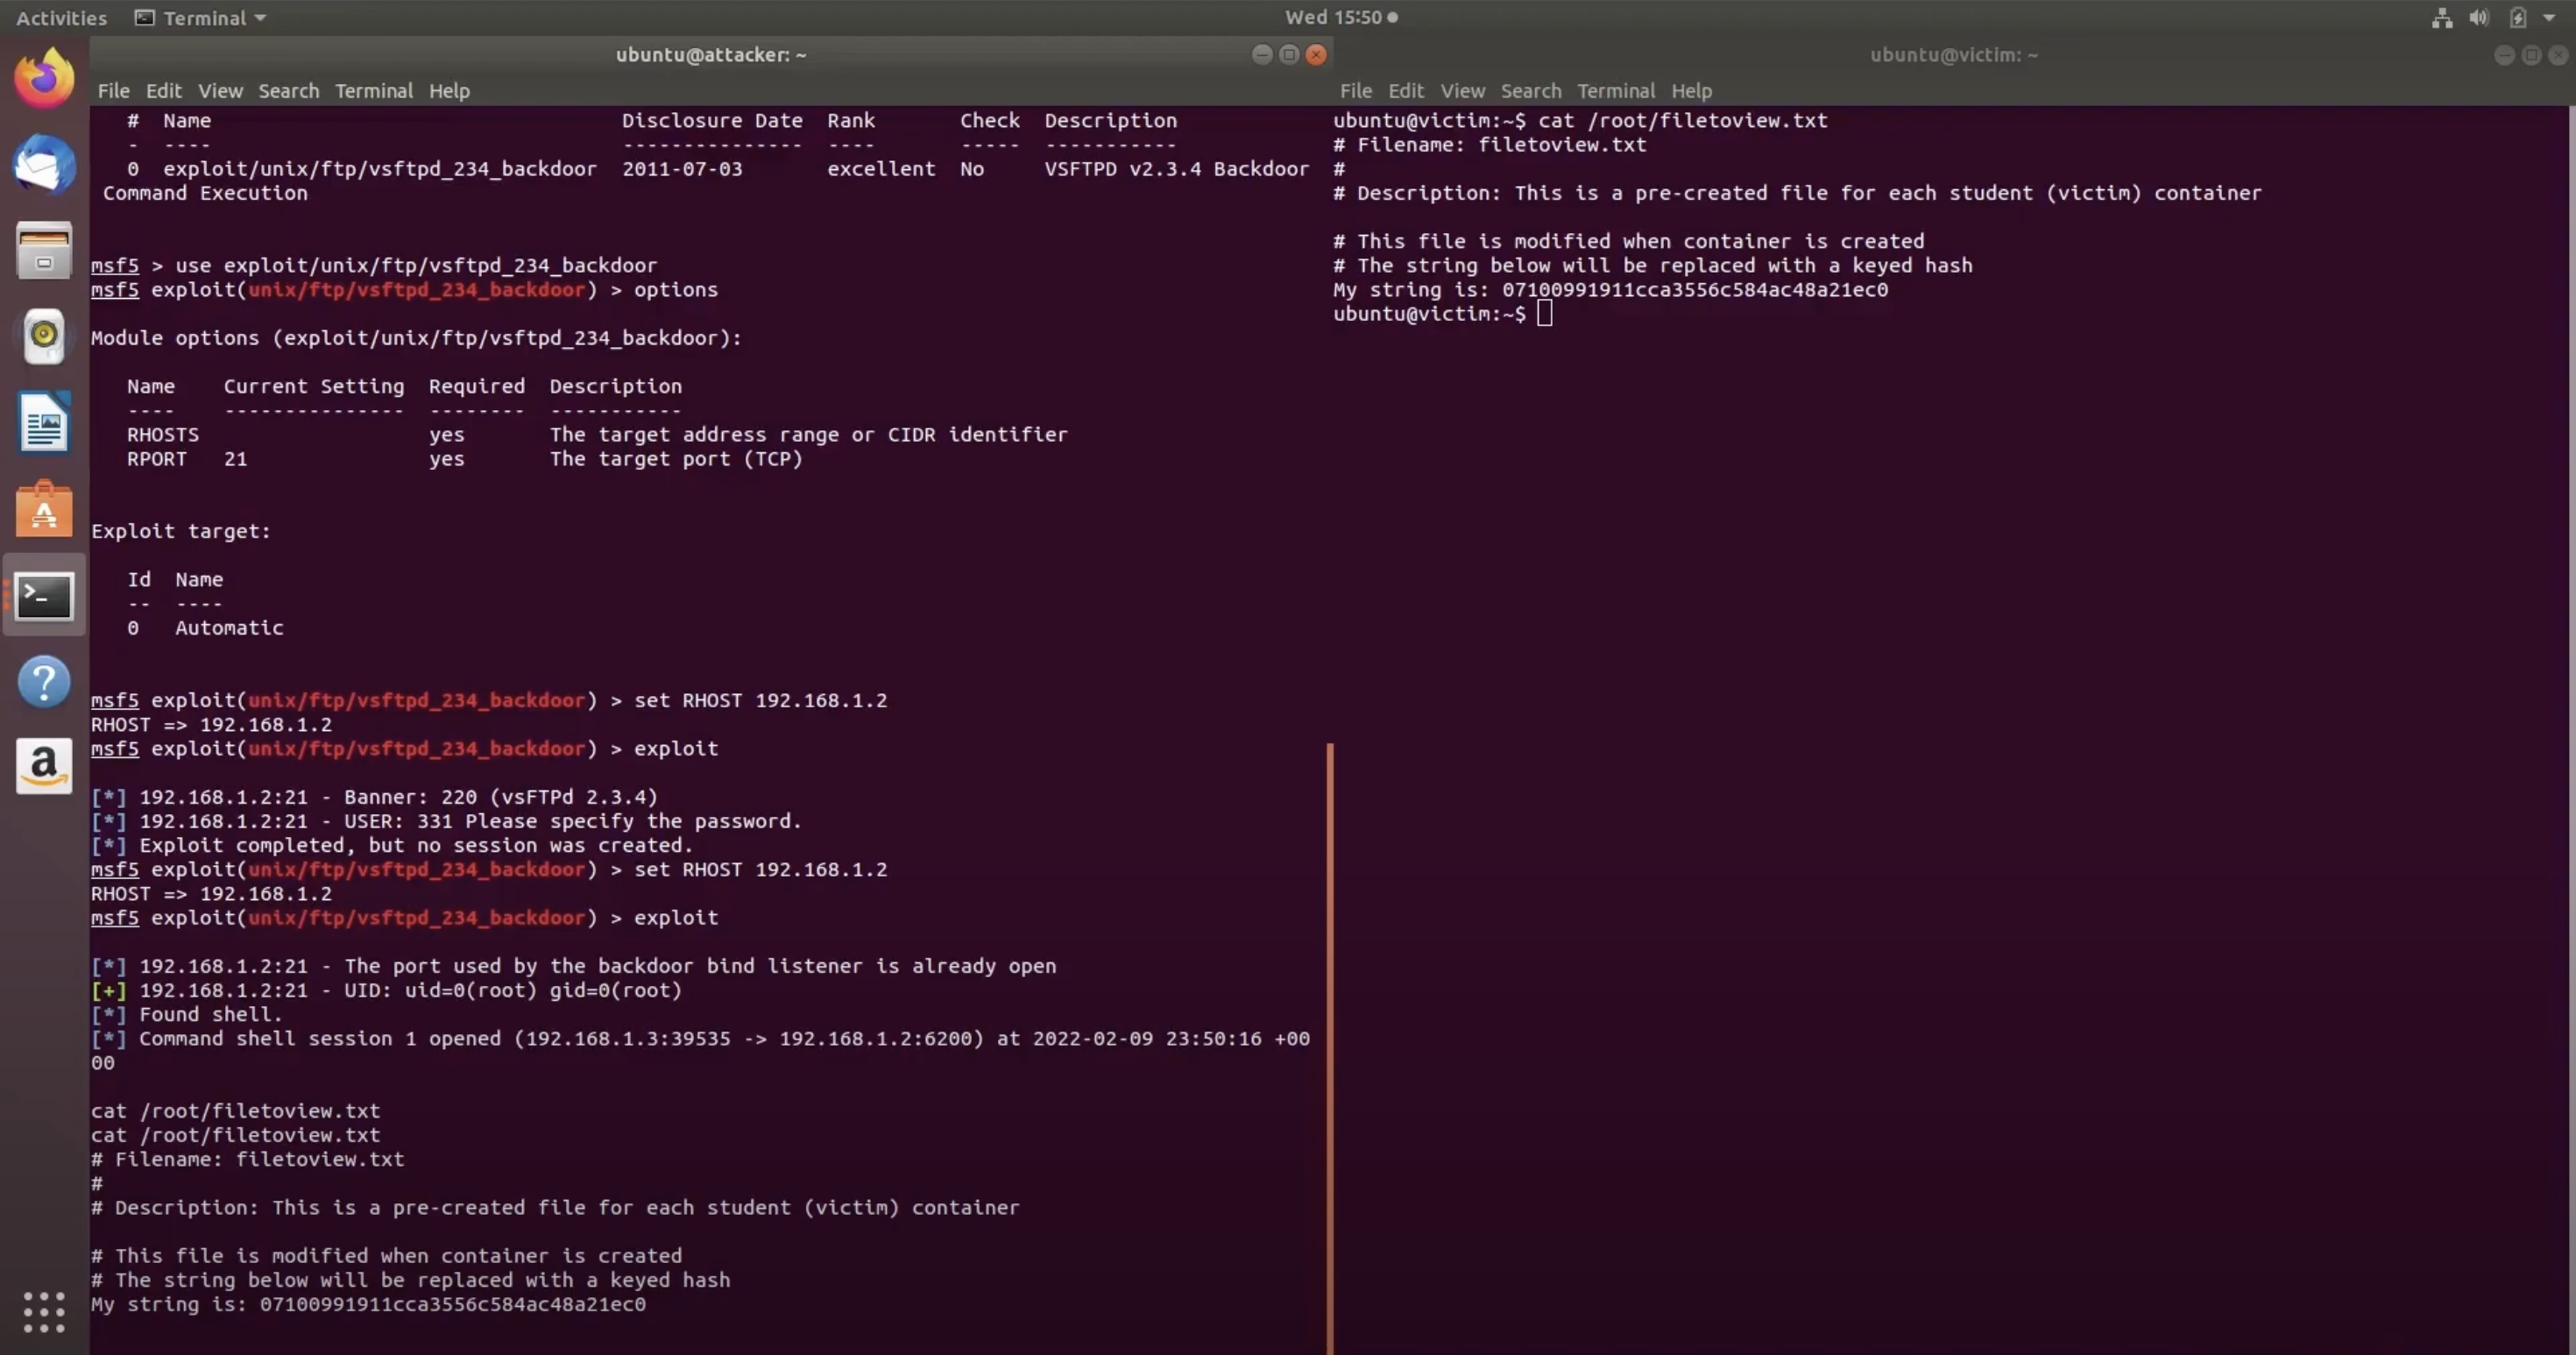
\includegraphics[width=0.7\textwidth]{images/11.png}
    \caption{VSFtpd Test}
\end{figure}

\subsubsection{Samba service (port 139)}
The Samba service, commonly running on port 139, provides file and print services for various clients in a network and allows interoperability between Unix/Linux and Windows systems. However, certain Samba configurations have been vulnerable to remote code execution attacks. In this lab, you will use Metasploit to exploit a vulnerability in the Samba usermap\_script feature, which can allow unauthorized access to the system.\\
To begin, start Metasploit and search for the usermap\_script exploit using the command search usermap\_script. Next, load the exploit with use exploit/multi/samba/usermap\_script. Then, view and configure the necessary options by running show options and set the target IP address with set RHOST 192.168.1.2. Once configured, run the exploit with exploit.\\
Upon successful execution, you will gain shell access to the target server. You can verify access by listing files in the root directory with ls /. This lab exercise demonstrates how attackers might exploit Samba vulnerabilities to gain unauthorized access, emphasizing the need to secure exposed services. 

\begin{figure}[h!]
    \centering
    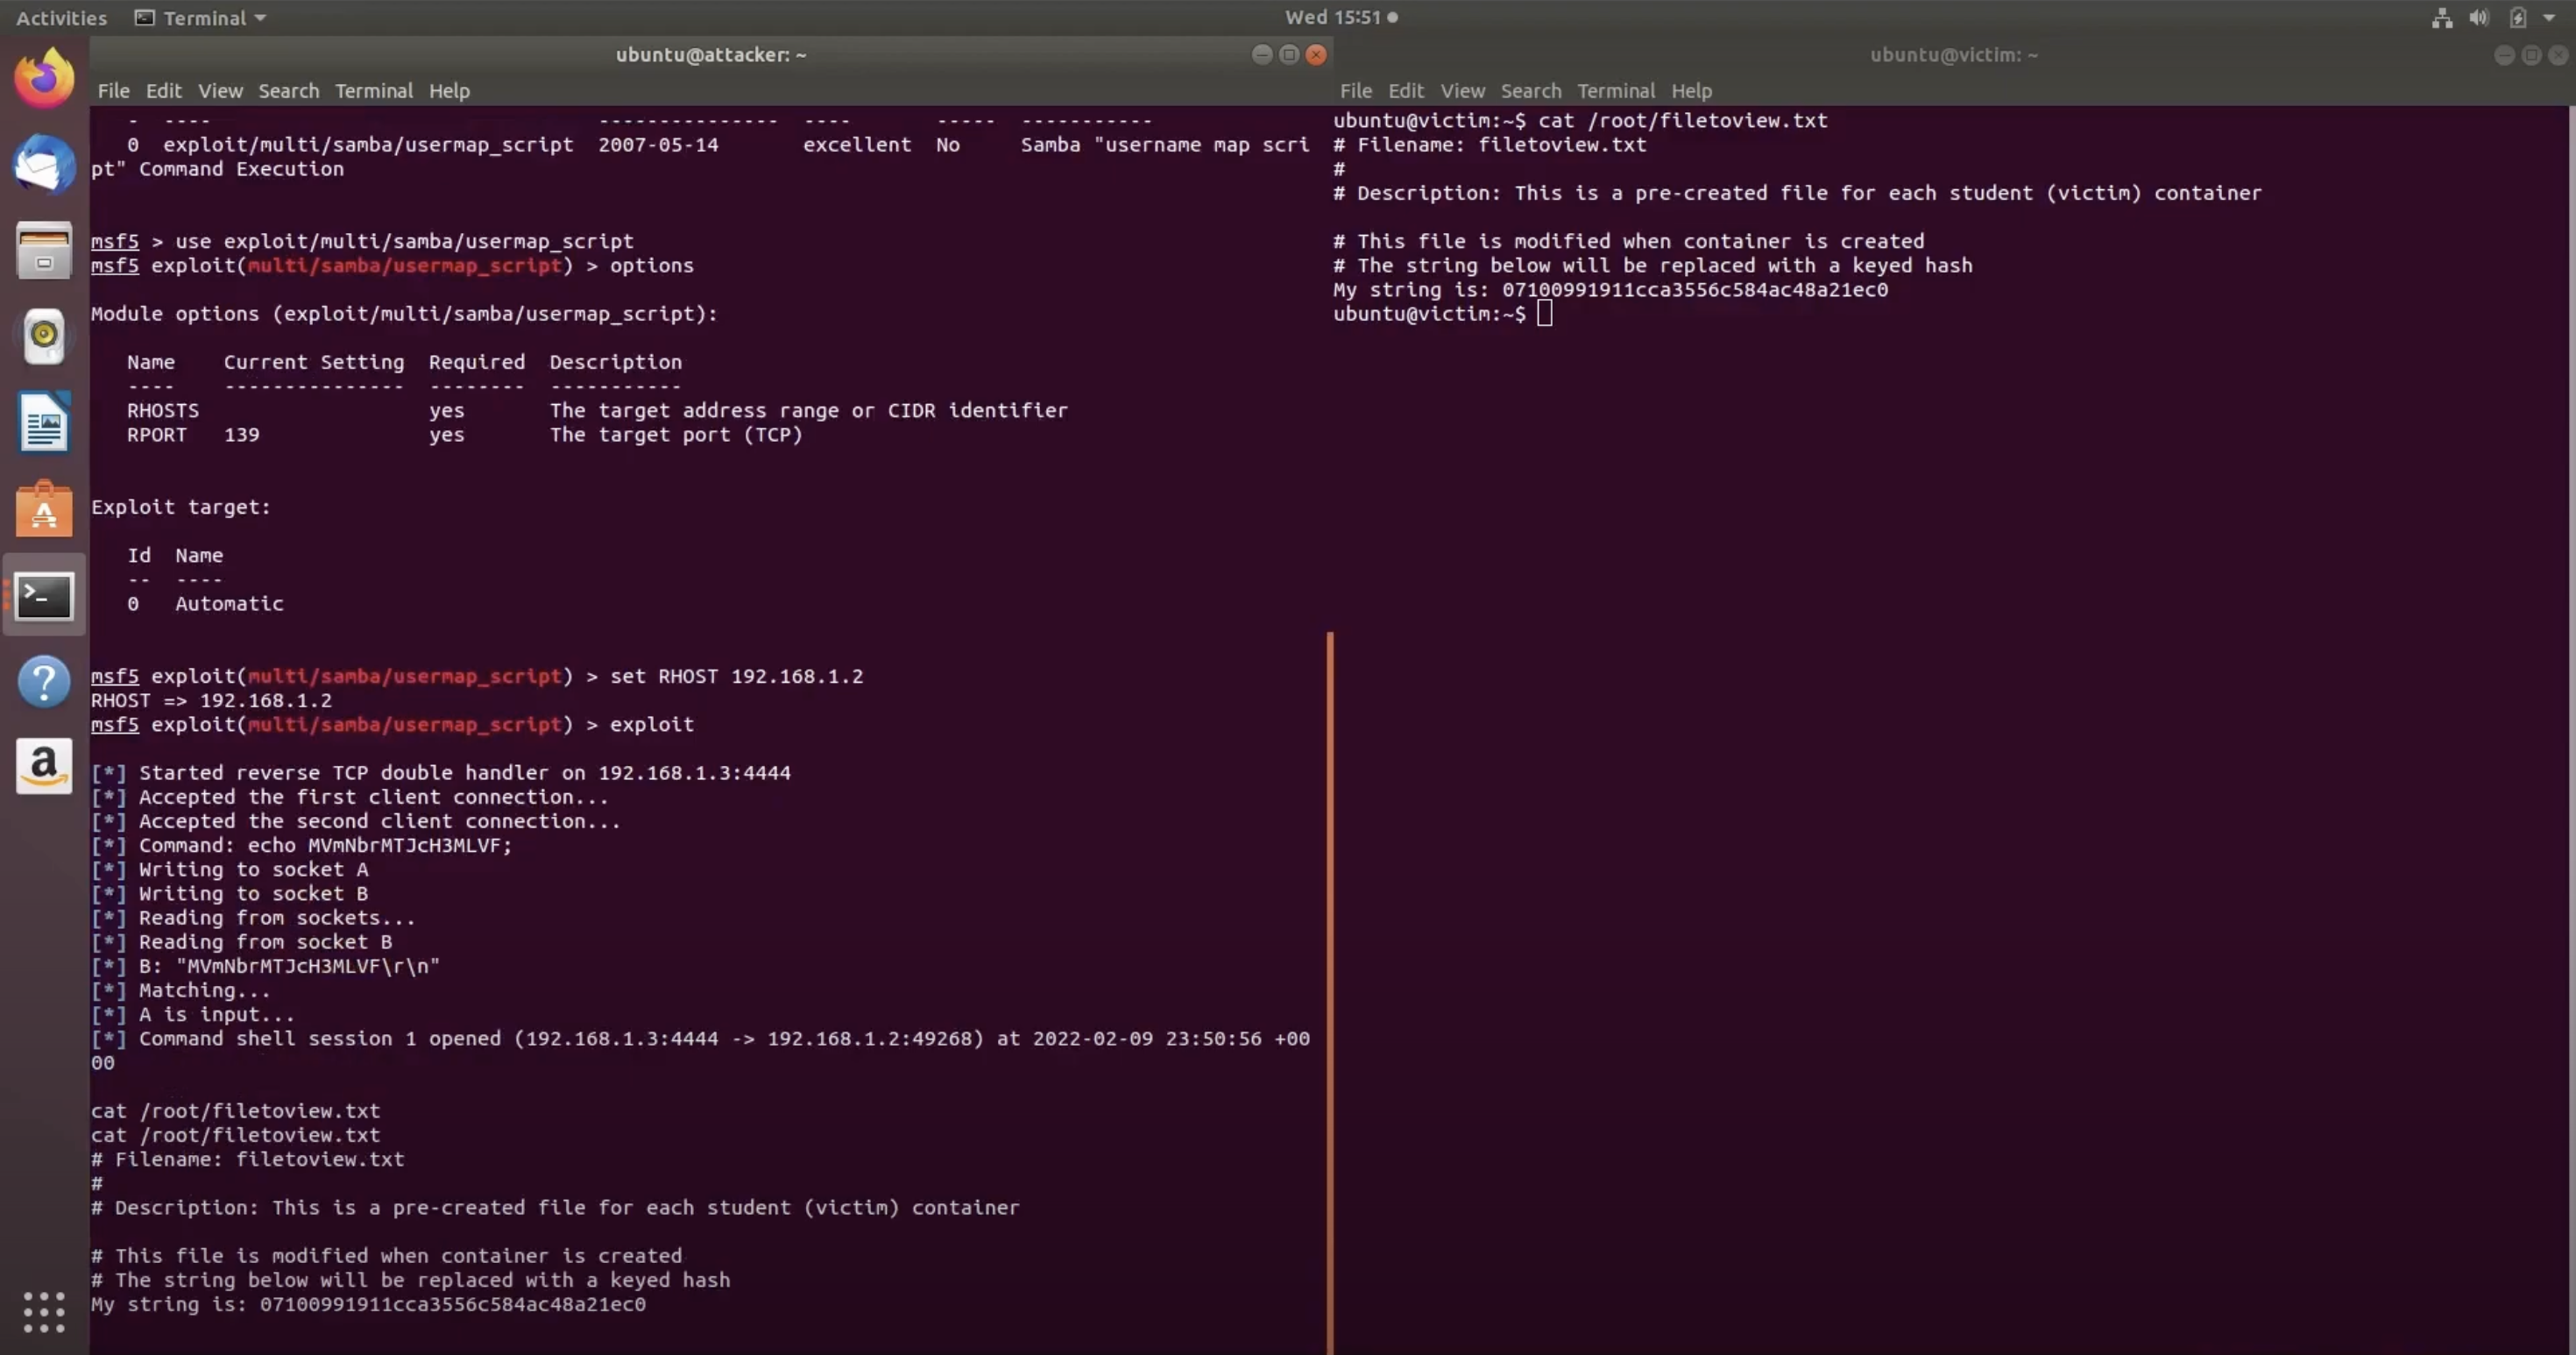
\includegraphics[width=0.7\textwidth]{images/12.png}
    \caption{Samba Test}
\end{figure}

\subsubsection{HTTP (php) service (port 80)}
The HTTP (PHP) service, typically running on port 80, can be vulnerable to specific exploits if misconfigured, particularly in PHP configurations that allow command injection. In this lab, you will use Metasploit to exploit a PHP CGI argument injection vulnerability, which can potentially grant remote access to a system.\\
To begin, launch Metasploit and search for the php\_cgi exploit by using the command search php\_cgi. Next, load the exploit with use exploit/multi/http/php\_cgi\_arg\_injection. After loading, view the required options by running show options, then set the target IP address using set RHOST 192.168.1.2. Once configured, execute the exploit by typing exploit.\\
Upon successful exploitation, a Meterpreter prompt will be displayed, indicating that you have gained control of the system. From the Meterpreter prompt, you can drop to a regular shell by typing shell. Once in the shell, you can display the contents of the root directory by entering ls /. This lab demonstrates how PHP vulnerabilities in web servers can lead to unauthorized access, emphasizing the importance of securing HTTP services. 

\break

\begin{figure}[h!]
    \centering
    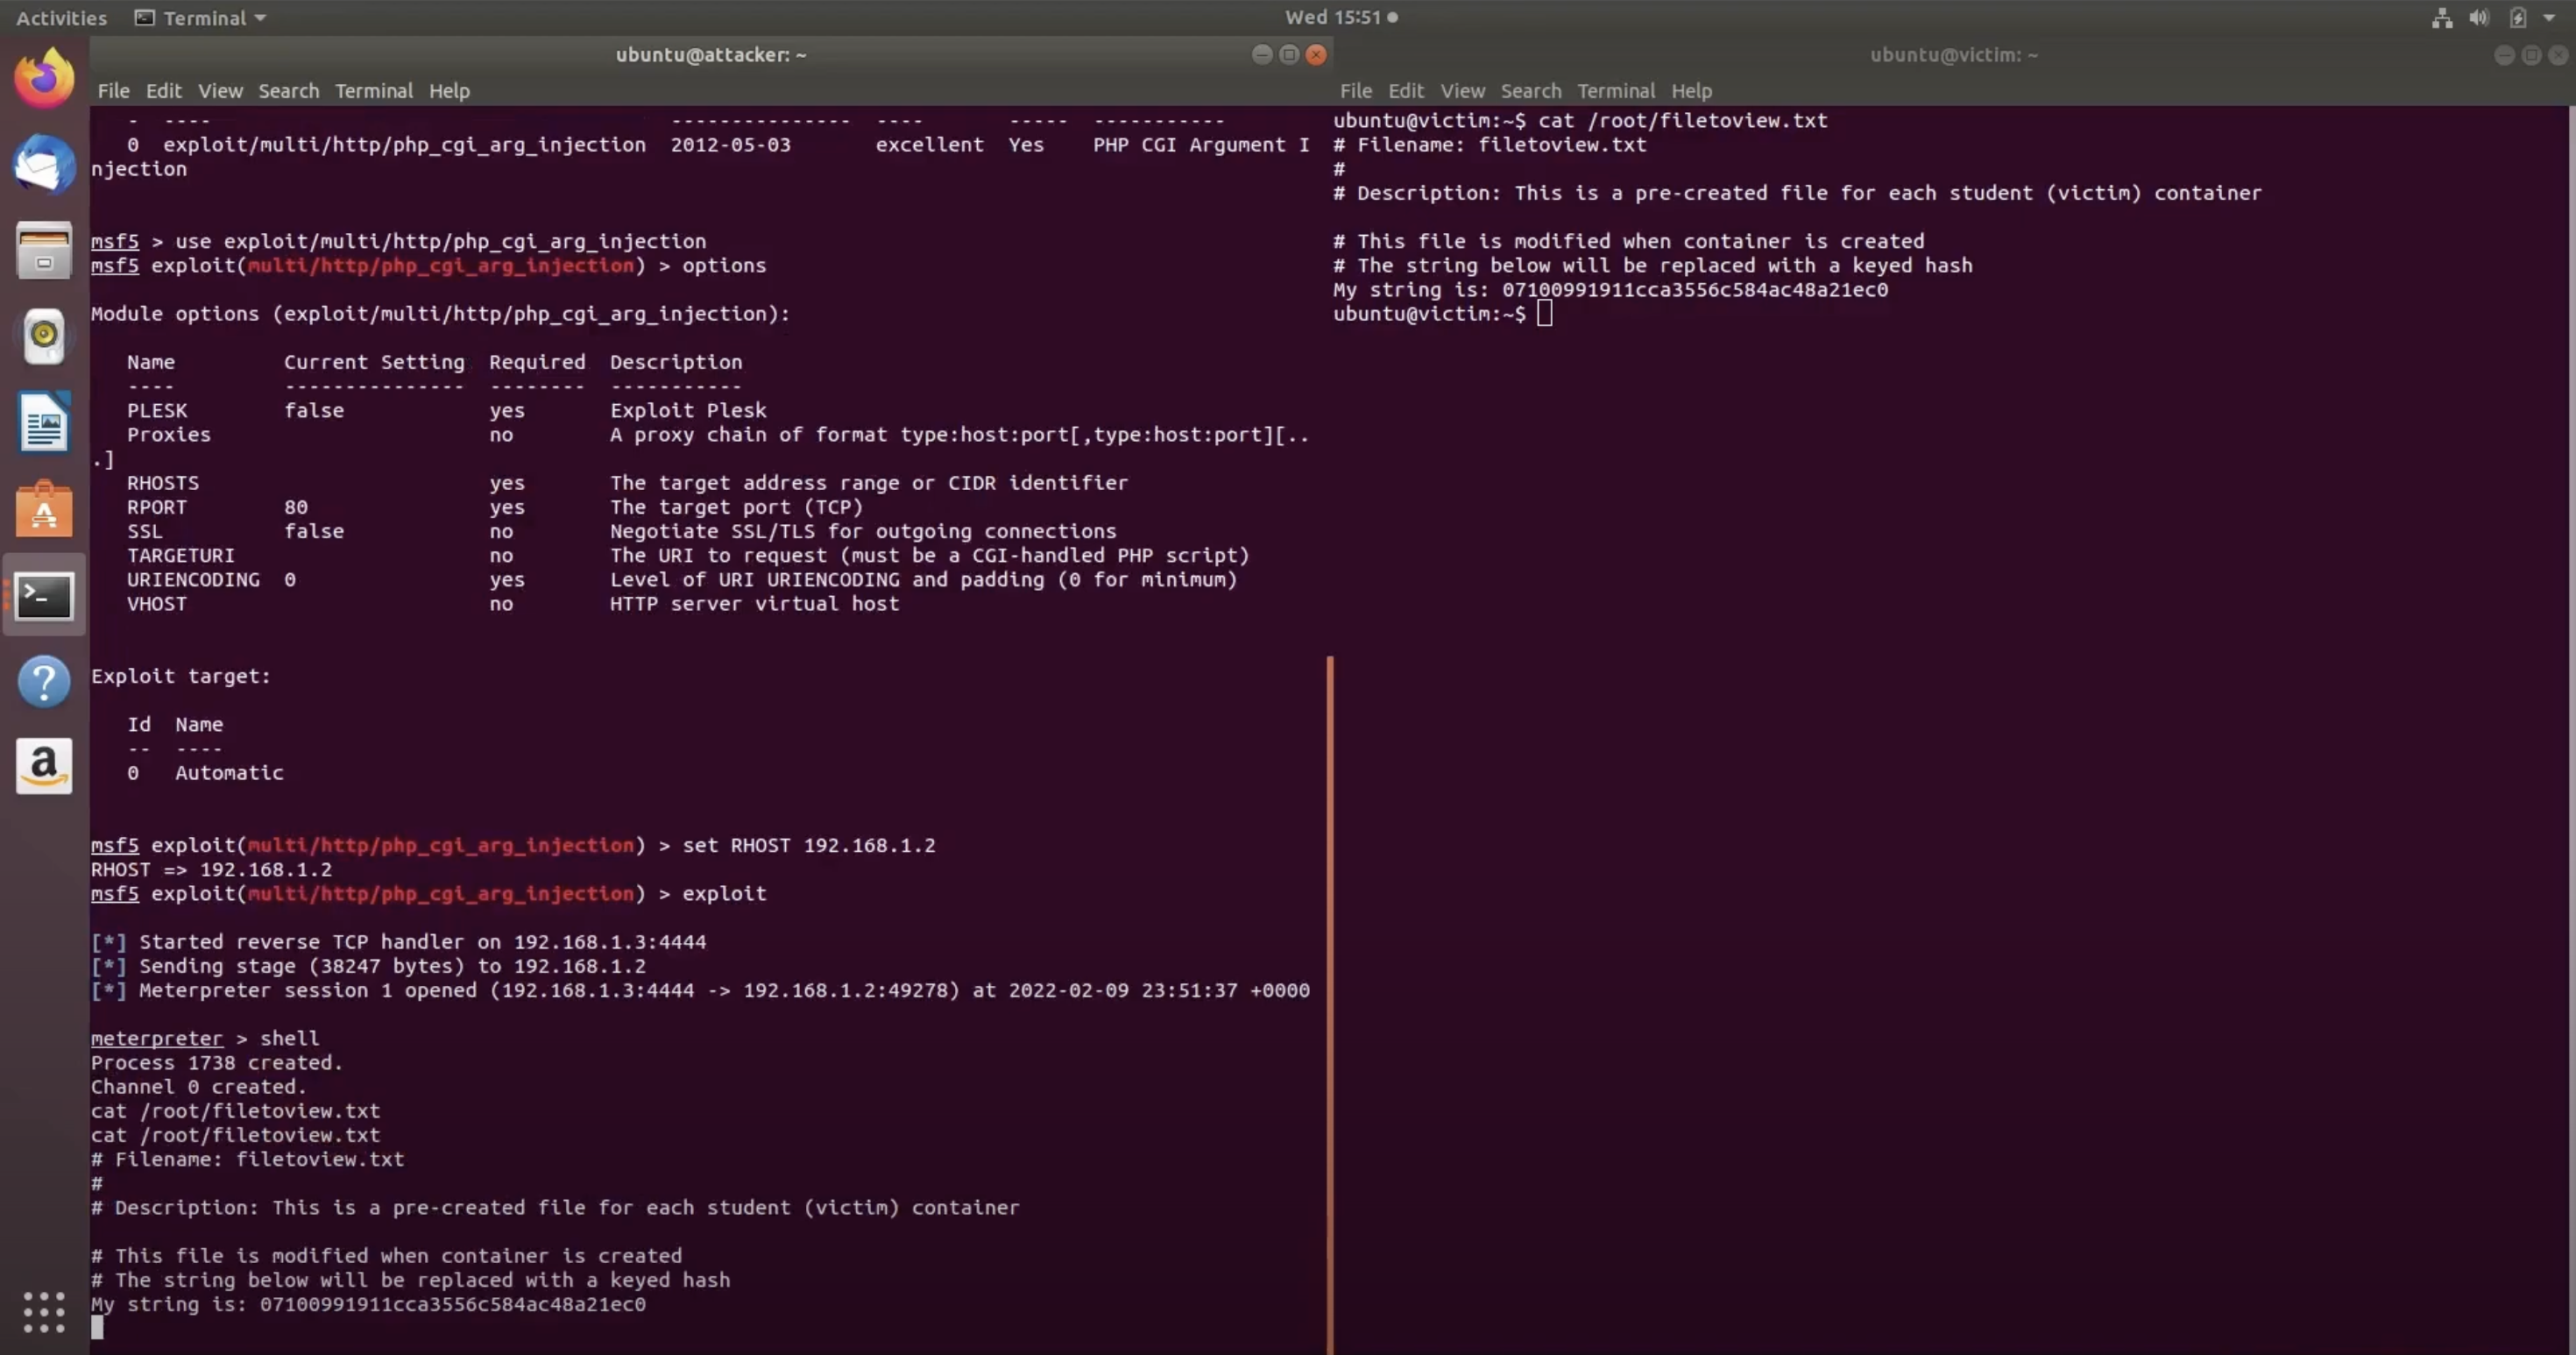
\includegraphics[width=0.7\textwidth]{images/13.png}
    \caption{HTTP Test}
\end{figure}

\subsubsection{Postgres service (port 5432)}
The PostgreSQL service, commonly running on port 5432, is a powerful open-source database system. If improperly secured, it can be vulnerable to remote code execution attacks. In this lab, you will use Metasploit to exploit a PostgreSQL vulnerability that may allow unauthorized access to the database server.\\
To start, launch Metasploit and search for the postgres\_payload exploit by using the command search postgres\_payload. Then, load the exploit with use exploit/linux/postgres/postgres\_payload. After loading the exploit, view the necessary options by running show options, and set the target IP address using set RHOST 192.168.1.2. Once configured, execute the exploit by typing exploit.\\
Upon successful exploitation, a Meterpreter prompt will appear, indicating that access has been gained. From the Meterpreter prompt, you can drop into a shell by typing shell. In the shell, display the contents of the root directory with ls /. This lab demonstrates how vulnerabilities in PostgreSQL can lead to unauthorized access, emphasizing the need to secure database services. 

\begin{figure}[h!]
    \centering
    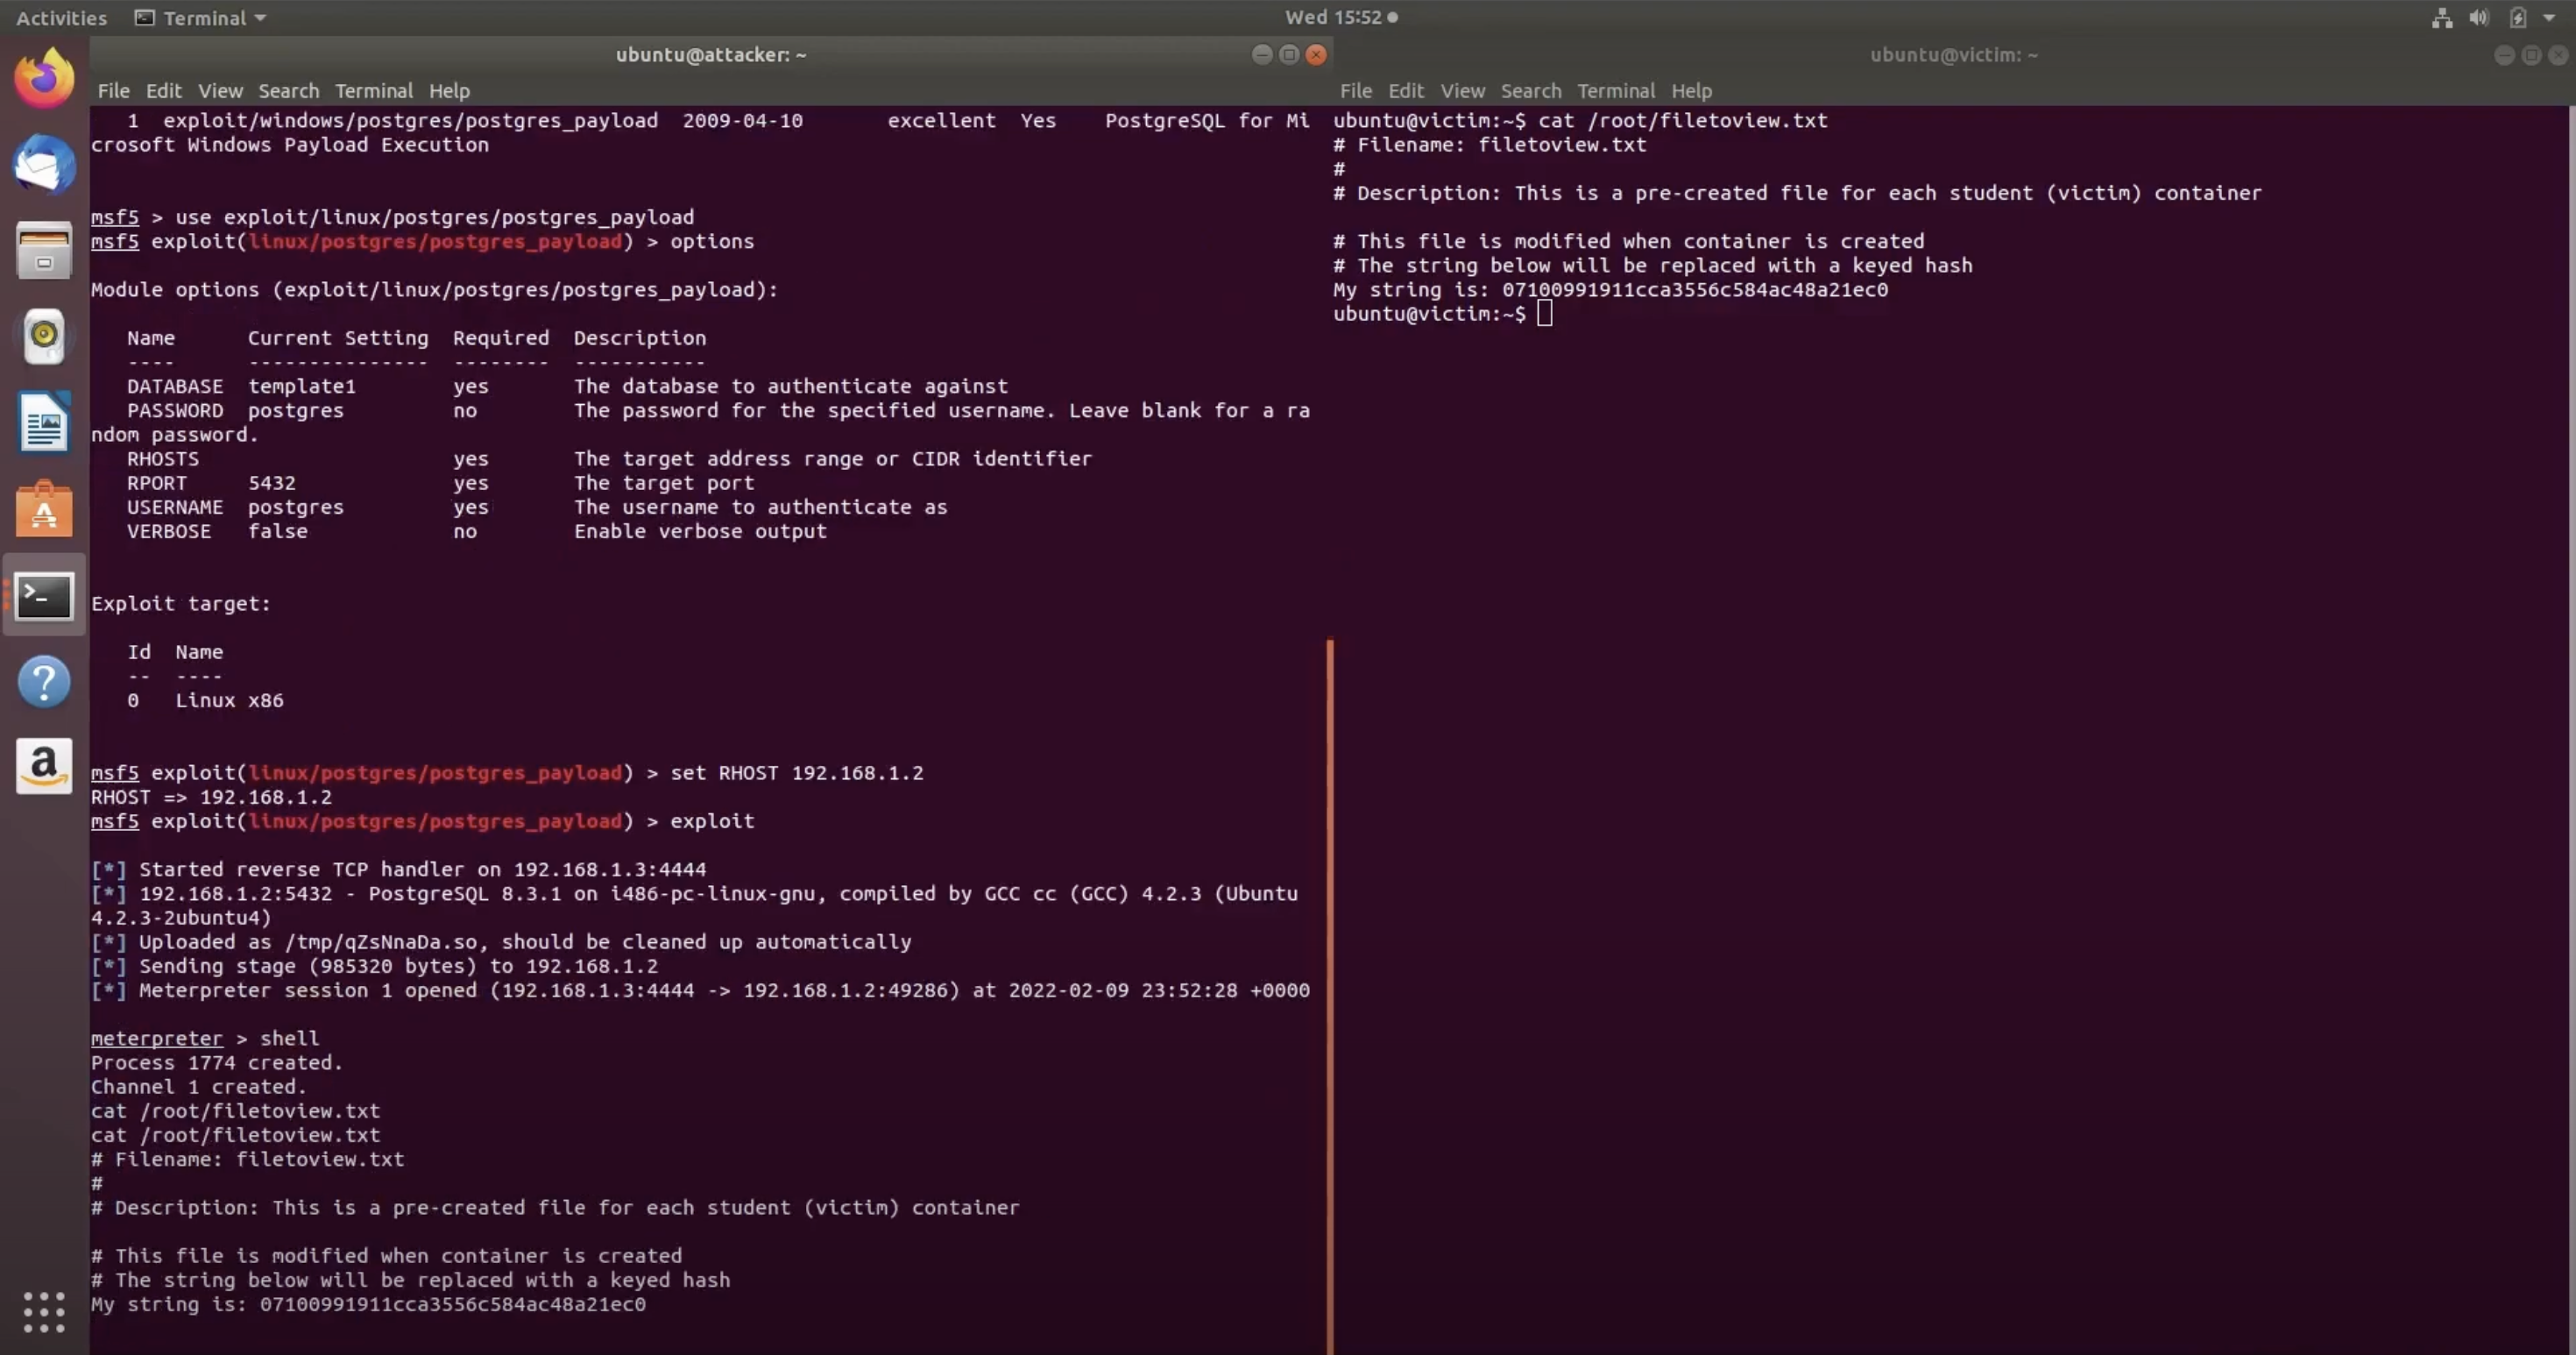
\includegraphics[width=0.7\textwidth]{images/14.png}
    \caption{Postgres Test}
\end{figure}

\newpage
\section{Snort}
\subsection{Objective}
The objective of this Snort laboratory is to provide hands-on experience in intrusion detection using Snort, a widely-used open-source network intrusion detection and prevention system. Through this lab, you will configure, test, and refine Snort rules to detect network threats in a controlled environment, gaining insight into how Snort monitors traffic and identifies potentially malicious activities.\\
The lab begins with an exploration of Snort’s functionality by running it with pre-configured rules to observe alerts generated during network scans. This helps you become familiar with Snort’s alerting capabilities and rule syntax. You will then create custom Snort rules, starting with a simple rule to detect all TCP traffic. This approach demonstrates the importance of specificity in rule configuration, as overly broad rules produce excessive alerts. The next step involves refining these rules to detect only specific patterns, such as attempts to access confidential data on the network.\\
To understand the limitations of Snort with encrypted sessions, you will generate SSL-encrypted traffic, observing that Snort cannot inspect or detect content within encrypted packets. This highlights the need for strategies, such as using a reverse proxy, to enable monitoring of encrypted traffic. The lab further explores configuring Snort to distinguish between internal and external traffic by customizing rules to allow internal access to sensitive content while generating alerts only for external access attempts, providing an essential layer of control in network security.\\
Finally, you will verify Snort’s detection capabilities for network scans, such as those conducted with nmap, across both internal and external segments of the network. By the end of this lab, you will gain practical skills in configuring Snort as a network intrusion detection tool, including writing effective rules, understanding challenges with encrypted traffic, and setting up rules to detect and respond to network threats. This experience reinforces critical concepts in network security and demonstrates real-world applications of intrusion detection and prevention systems.

\subsection{Starting the Lab}
To star the lab, we use the command in the Labtainer Terminal:
\[\texttt{labtainer snort}\]
After that, this three windows are opened:

\begin{figure}[h!]
    \centering
    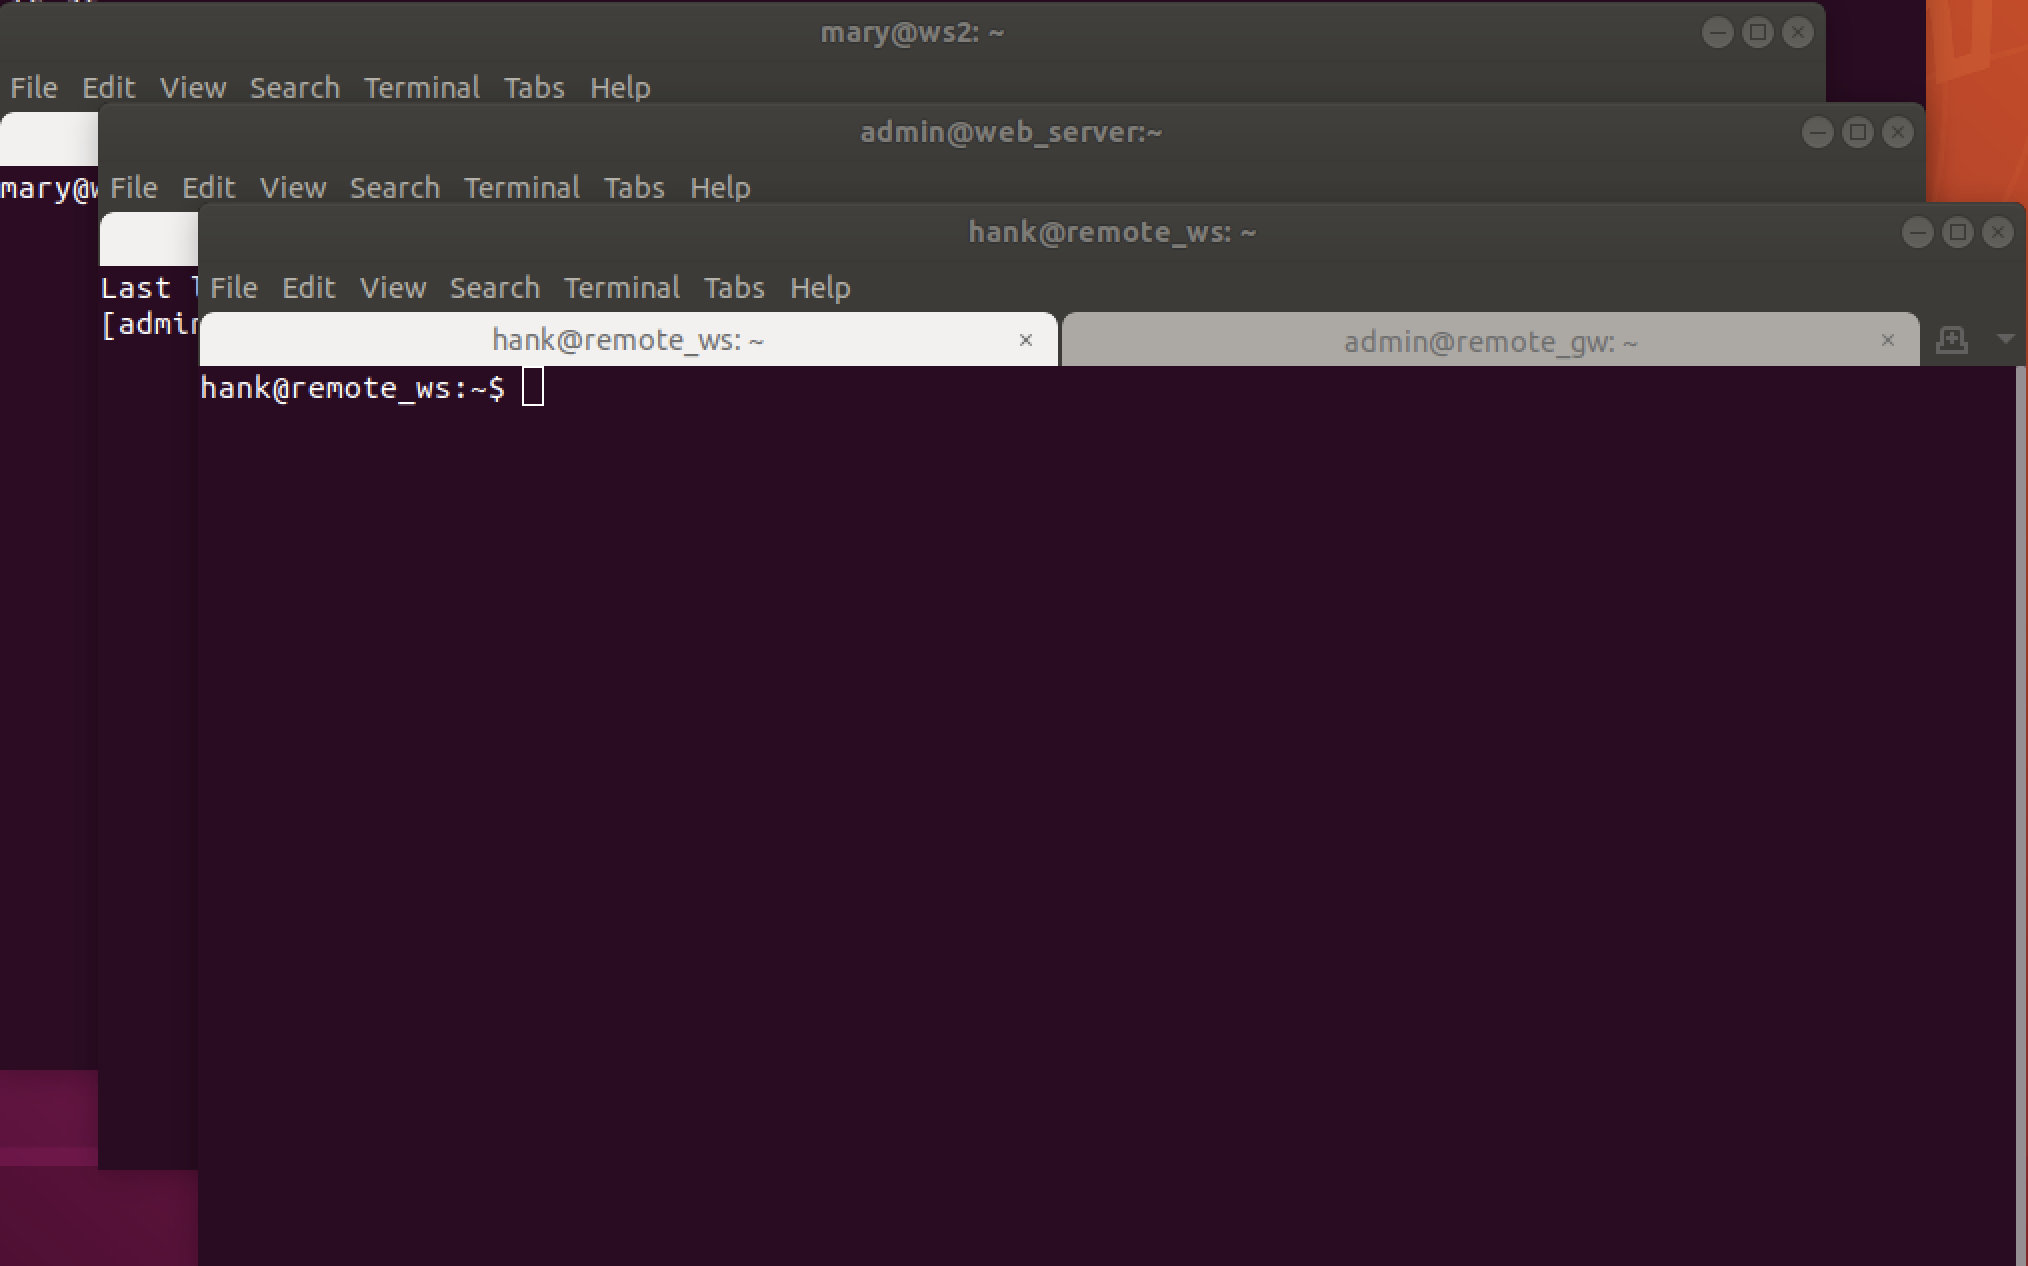
\includegraphics[width=0.7\textwidth]{images/15.png}
    \caption{Working Windows}
\end{figure}

\subsection{Lab Tasks}
\subsubsection{Starting Snort}
The purpose of this initial step is to familiarize ourselves with Snort’s basic operation in Network Intrusion Detection Mode. We start Snort using a script (./start\_snort.sh) that launches Snort in IDS mode, displaying alerts directly in the terminal. This enables us to see how Snort outputs real-time alerts for network activity that matches any pre-configured rules. To stop Snort, we use Ctrl+C, which will allow us to modify configurations or add new rules as needed. This task provides a foundational understanding of Snort’s alerting process and console output.\\
In \textbf{tom@snort} directory, we use the command below to start Snort:
\[\texttt{.\/start\_snort.sh}\]

\subsubsection{Pre-Configure Snort Rules}
Snort includes a set of pre-configured rules designed to detect various network anomalies, such as unauthorized access attempts or port scans. In this task, we observe how these default rules function by performing a network scan from a remote workstation (e.g., using nmap). Snort’s output will show alerts triggered by the scan activity, allowing us to identify which specific rules are activated. Reviewing these alerts and the associated rules helps us understand how Snort uses pre-existing configurations to detect common network security threats.\\
For this, we use, in \textbf{hank@remote\_ws}:
\[\texttt{sudo nmap www.example.com}\]

\begin{figure}[h!]
    \centering
    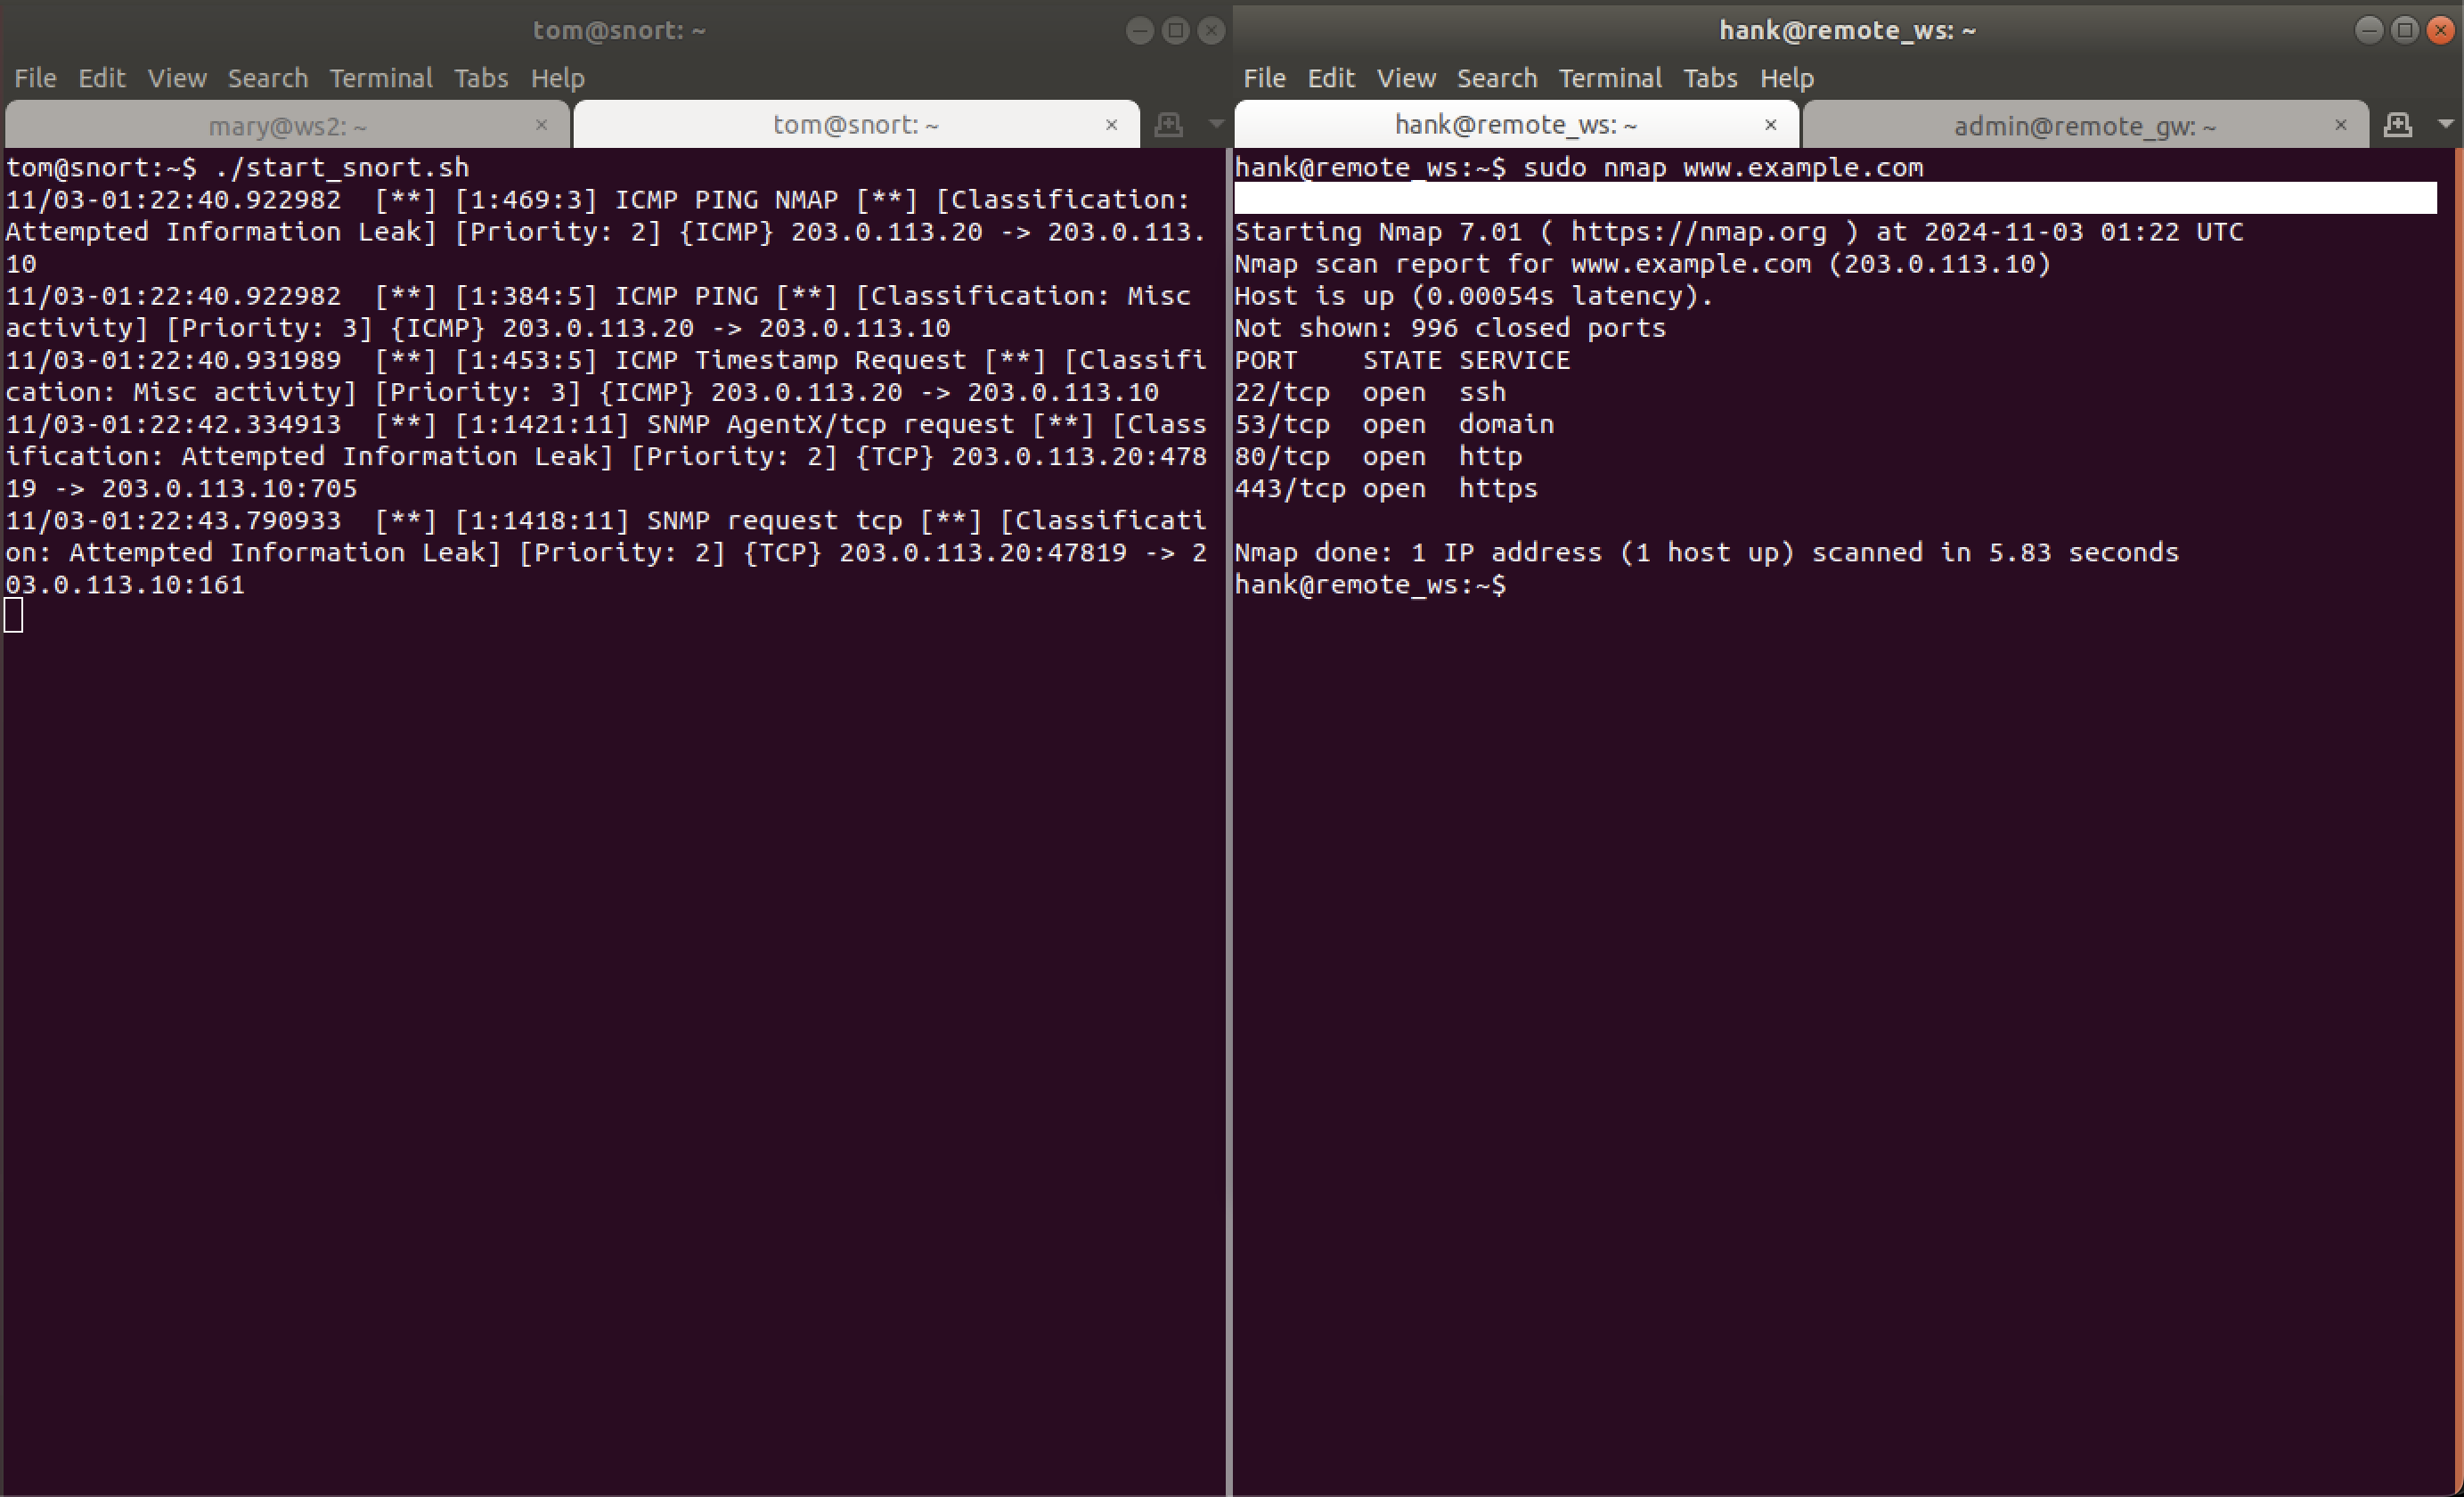
\includegraphics[width=0.7\textwidth]{images/16.png}
    \caption{Nmap Test}
\end{figure}
In this case, we can note the \texttt{ICMP PING NMAP} working properly with the configurations of the program.

\subsubsection{Write a Simple (Bad) Rule}
In this task, we write a basic Snort rule that detects all TCP packets. This broad rule is designed to illustrate how overly general rules can lead to excessive, irrelevant alerts. By creating the rule (alert tcp any any -> any any (msg:"TCP detected"; sid:00002;)) and observing its behavior, we see that Snort generates a flood of alerts due to the rule’s lack of specificity. This exercise emphasizes the importance of creating targeted rules, as overly broad detection criteria can overwhelm the alert system and reduce the IDS’s effectiveness. After testing, we remove or comment out this rule to avoid unnecessary logging.
So, we use:
\[\texttt{sudo vim /etc/snort/rules/local.rules}\]
And we add the rule:
\[\texttt{alert tcp any any -> any any (msg:"TCP detected"; sid:00002;)}\]

\begin{figure}[h!]
    \centering
    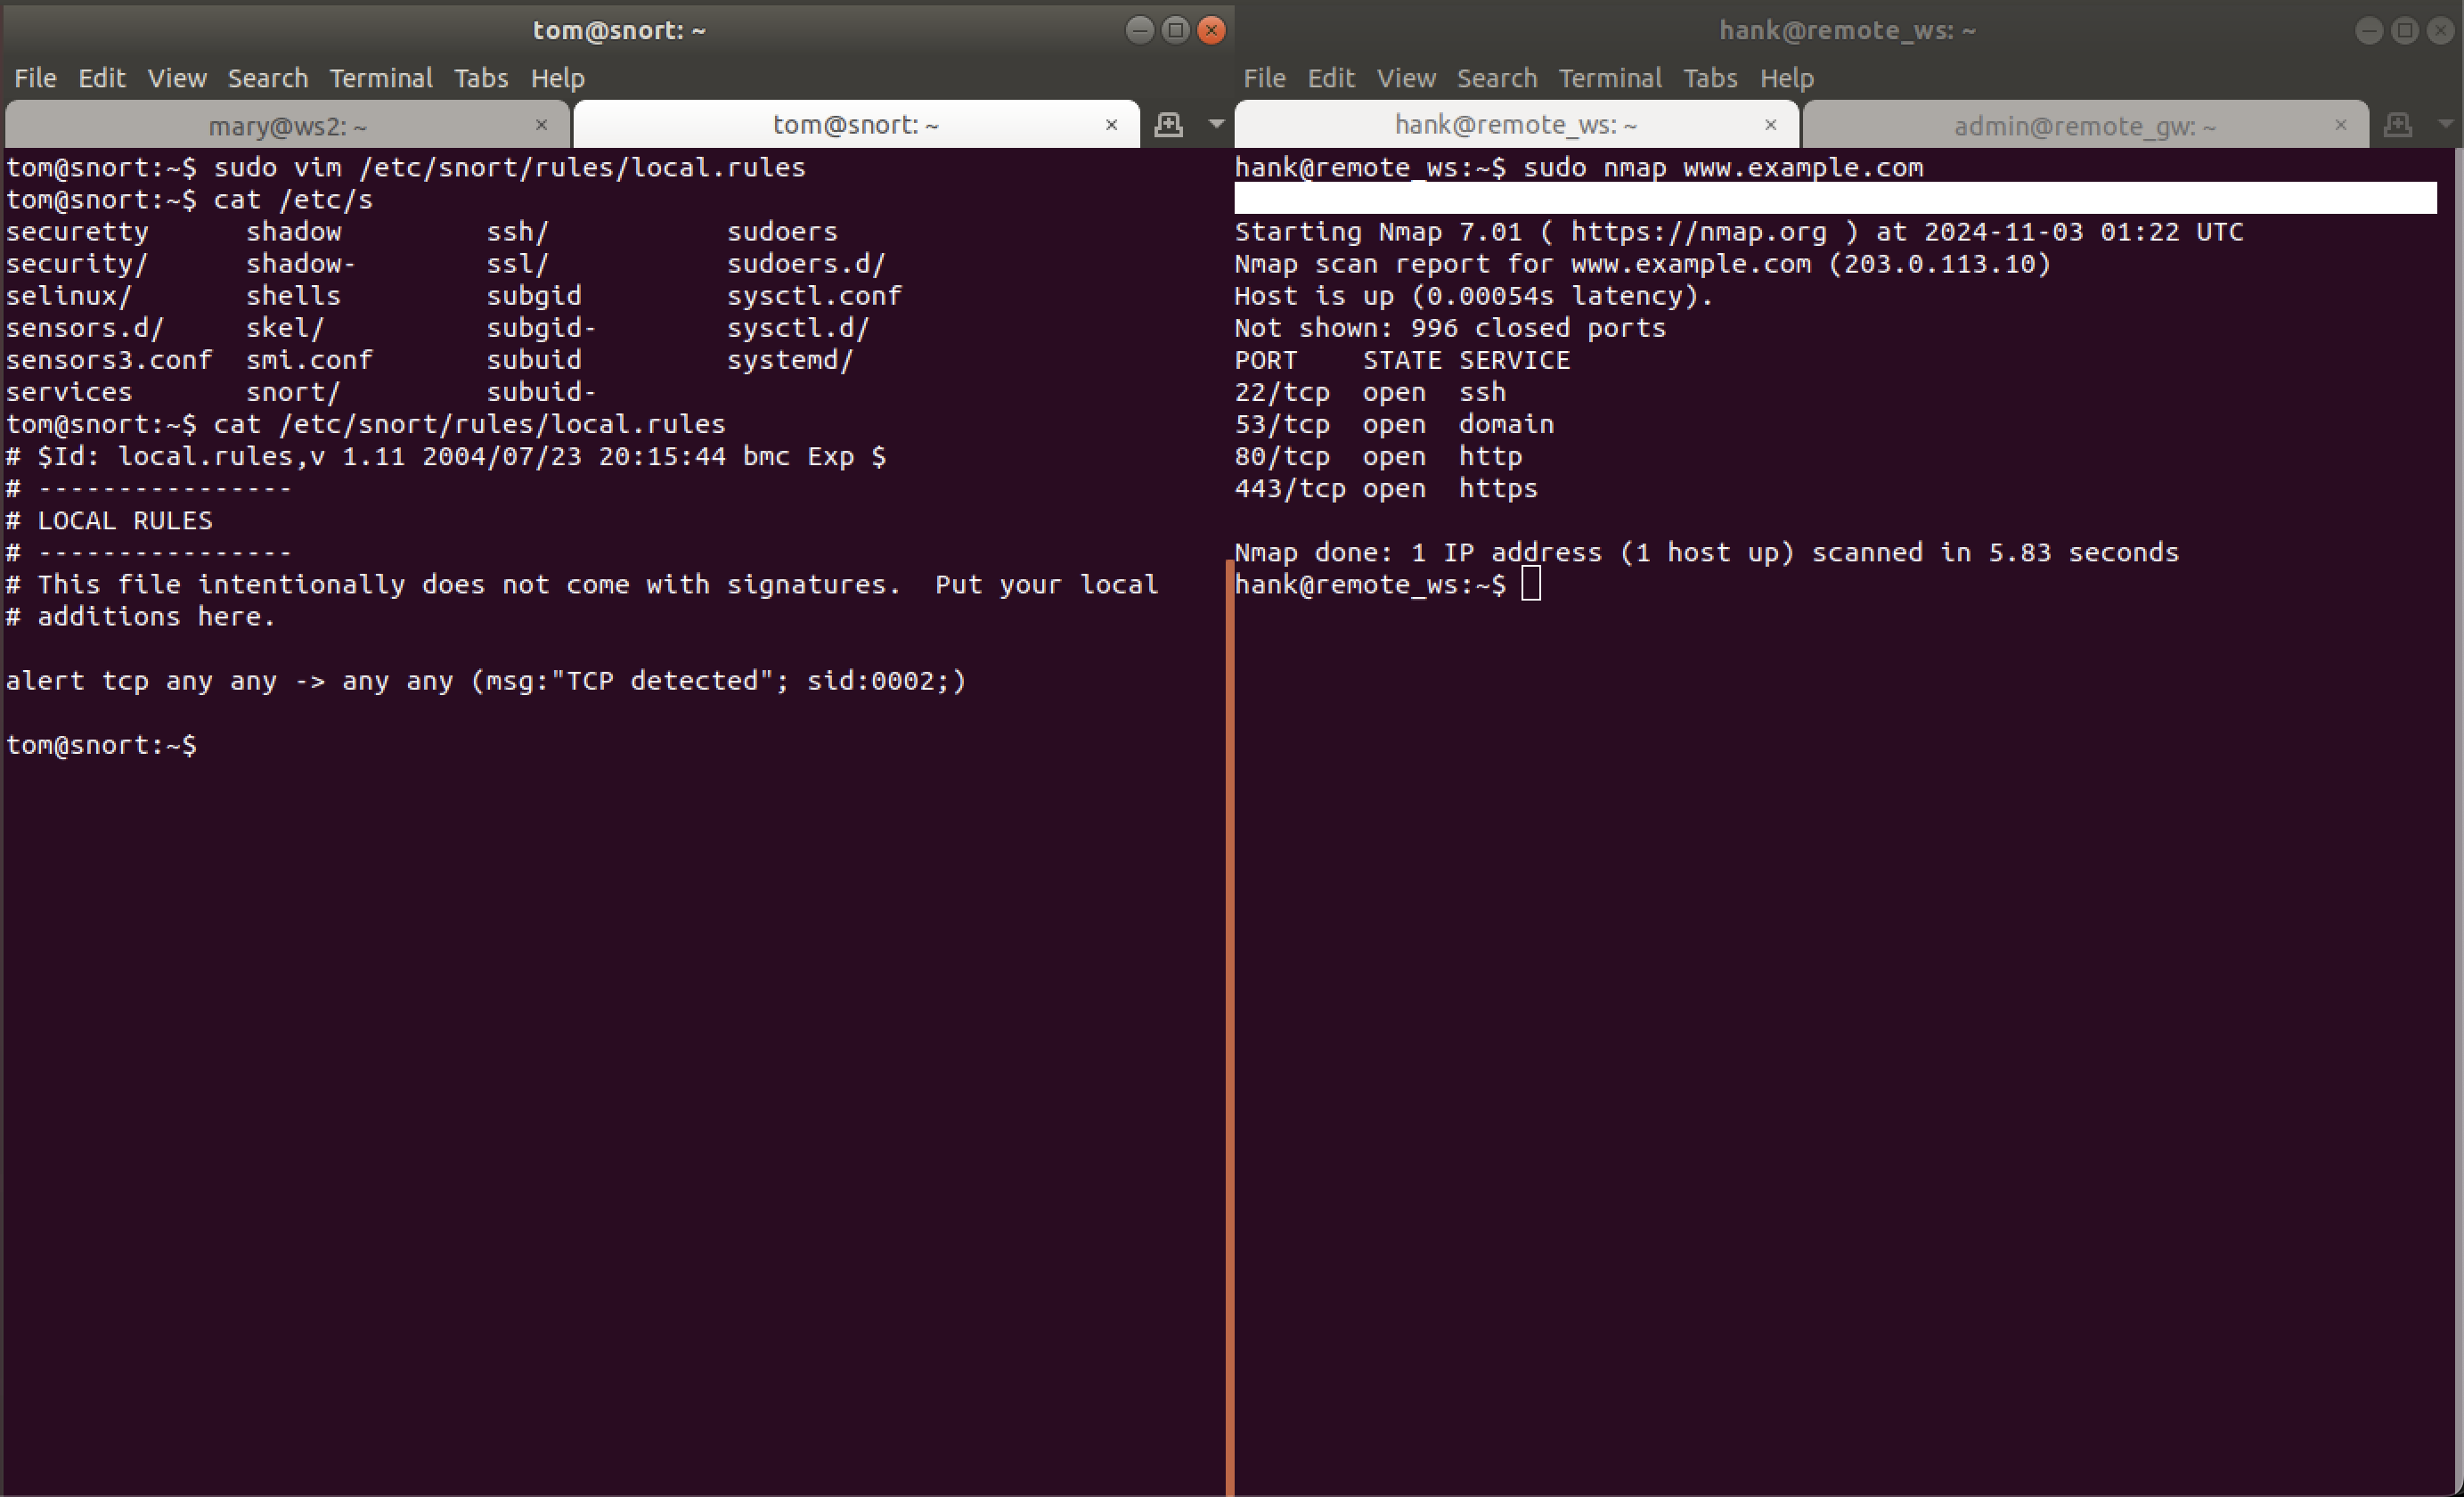
\includegraphics[width=0.7\textwidth]{images/17.png}
    \caption{Basic Rule}
\end{figure}

After that, we can verify the Rule with:
\[\texttt{./start\_snort.sh}\]
\[\texttt{firefox www.example.com}\]
Wich results in:

\begin{figure}[h!]
    \centering
    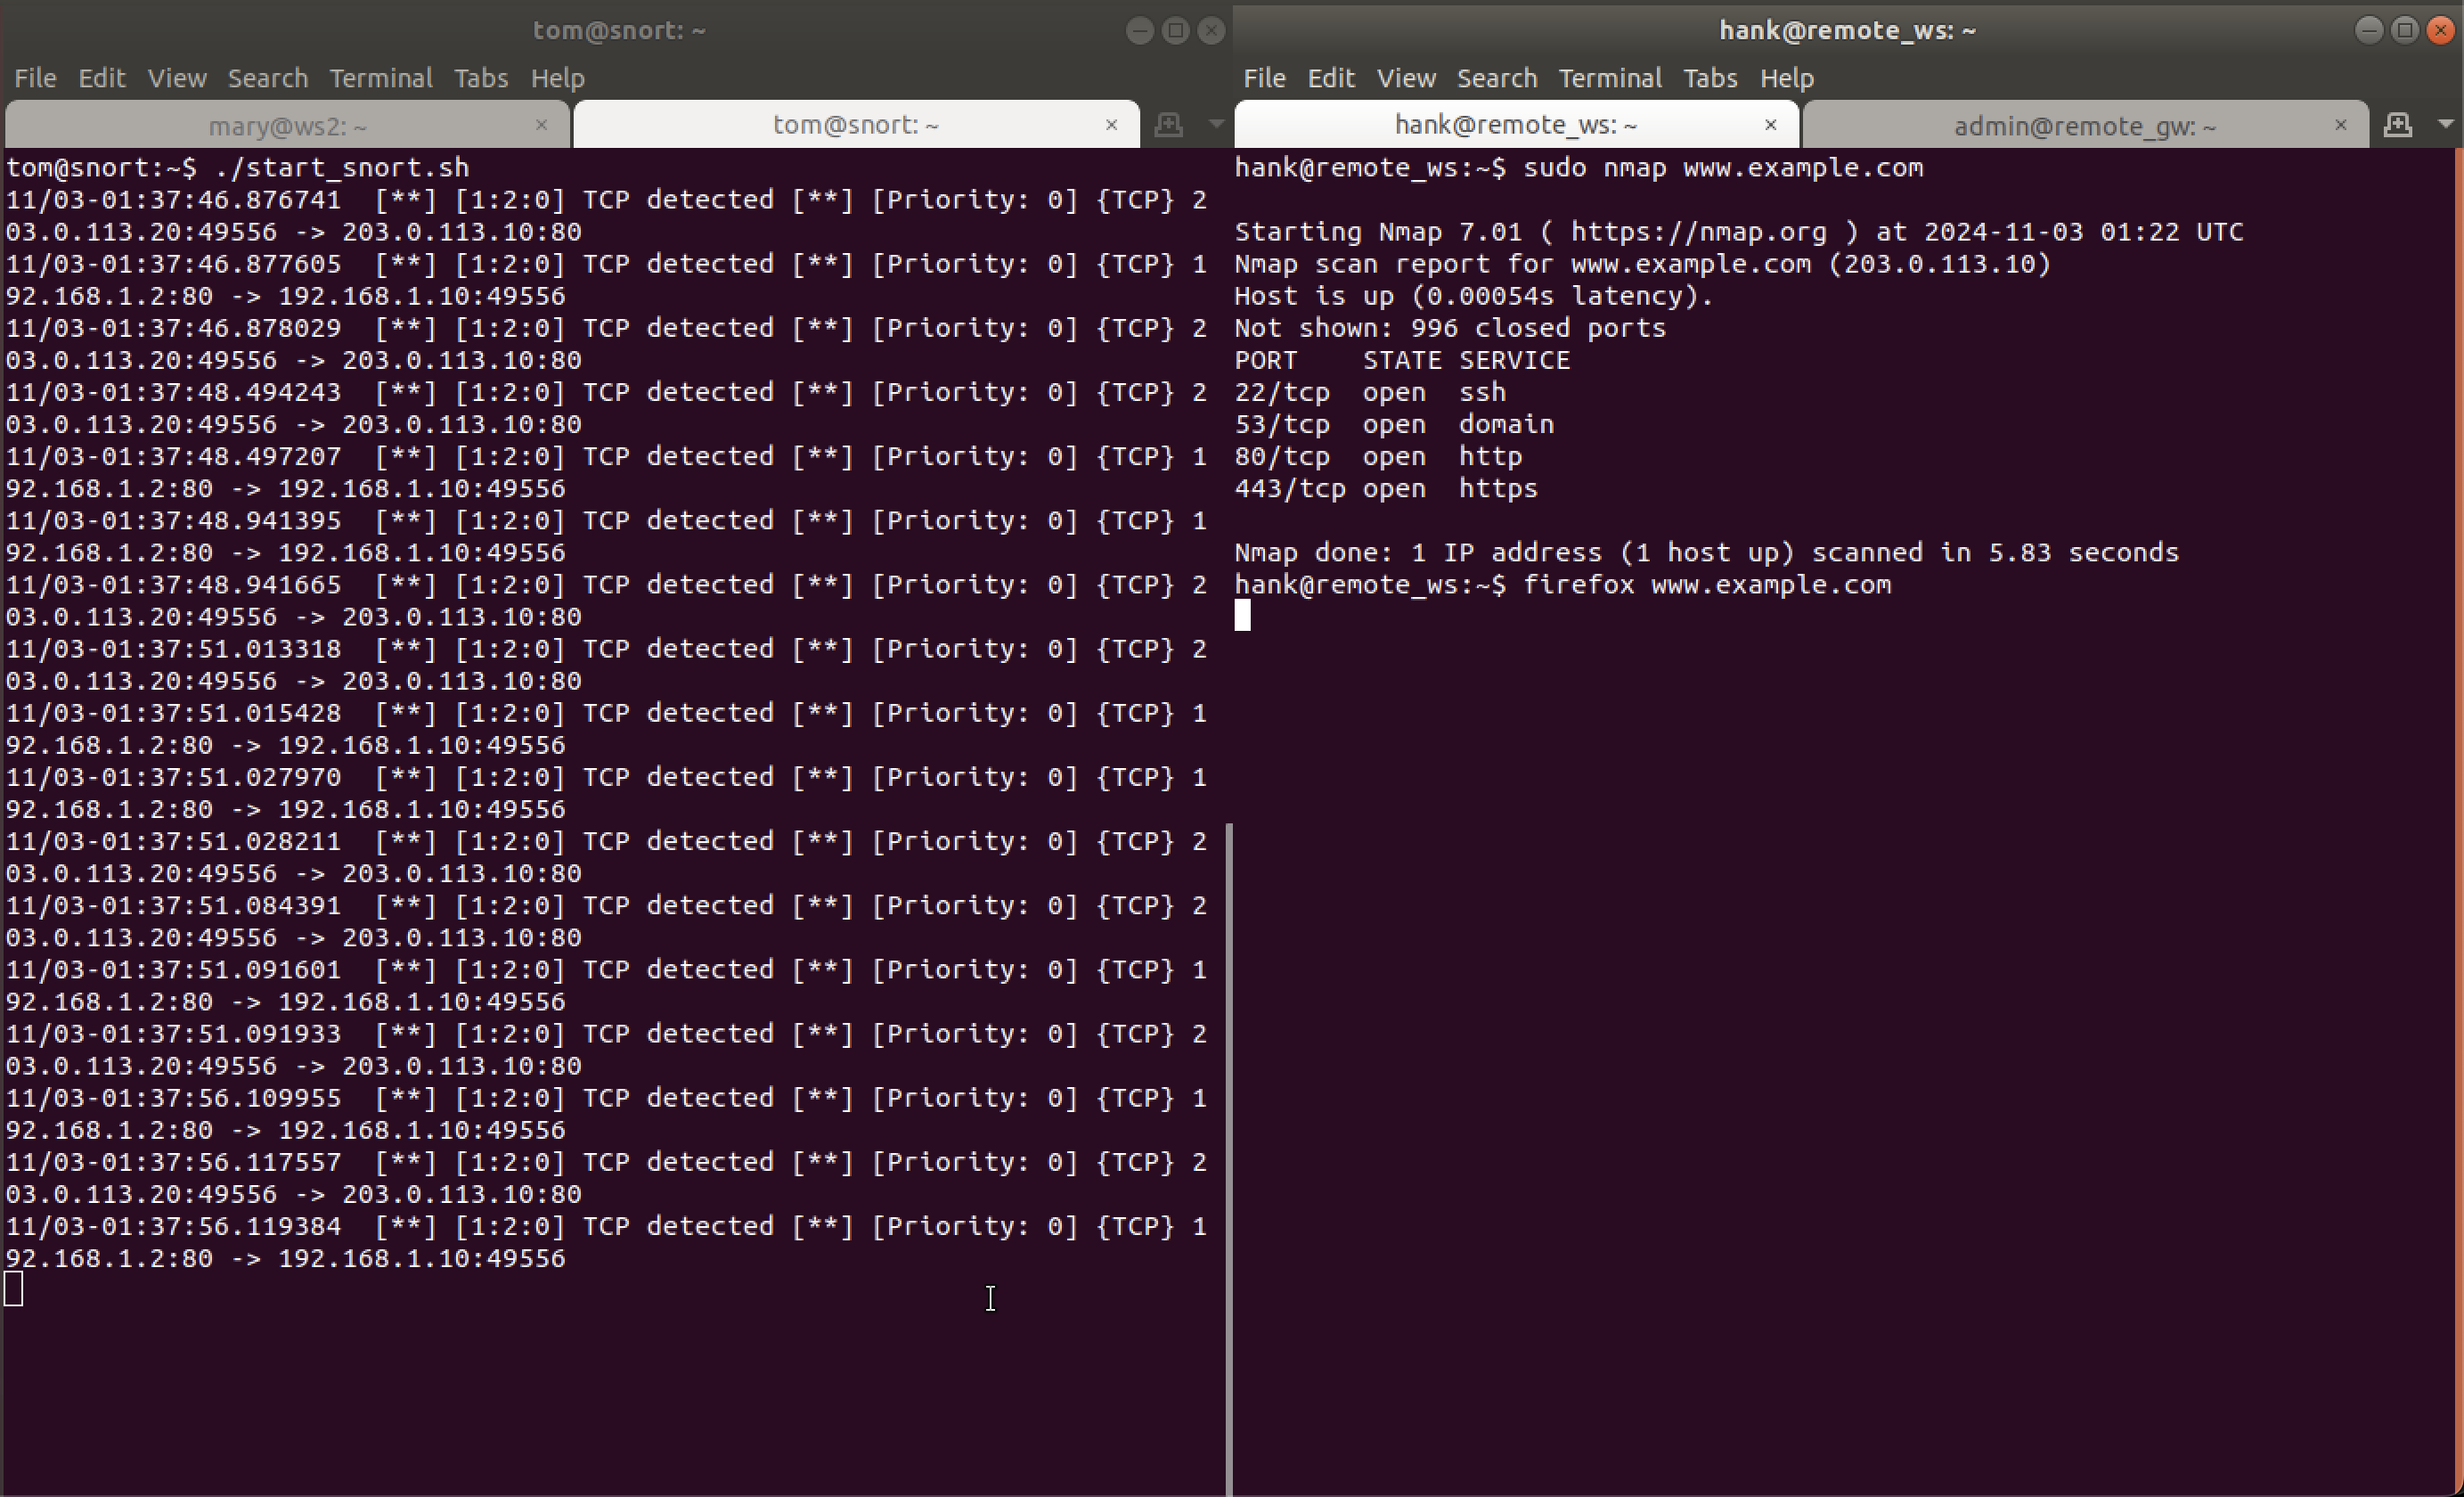
\includegraphics[width=0.7\textwidth]{images/18.png}
    \caption{Rule Test}
\end{figure}

\break 

\begin{figure}[h!]
    \centering
    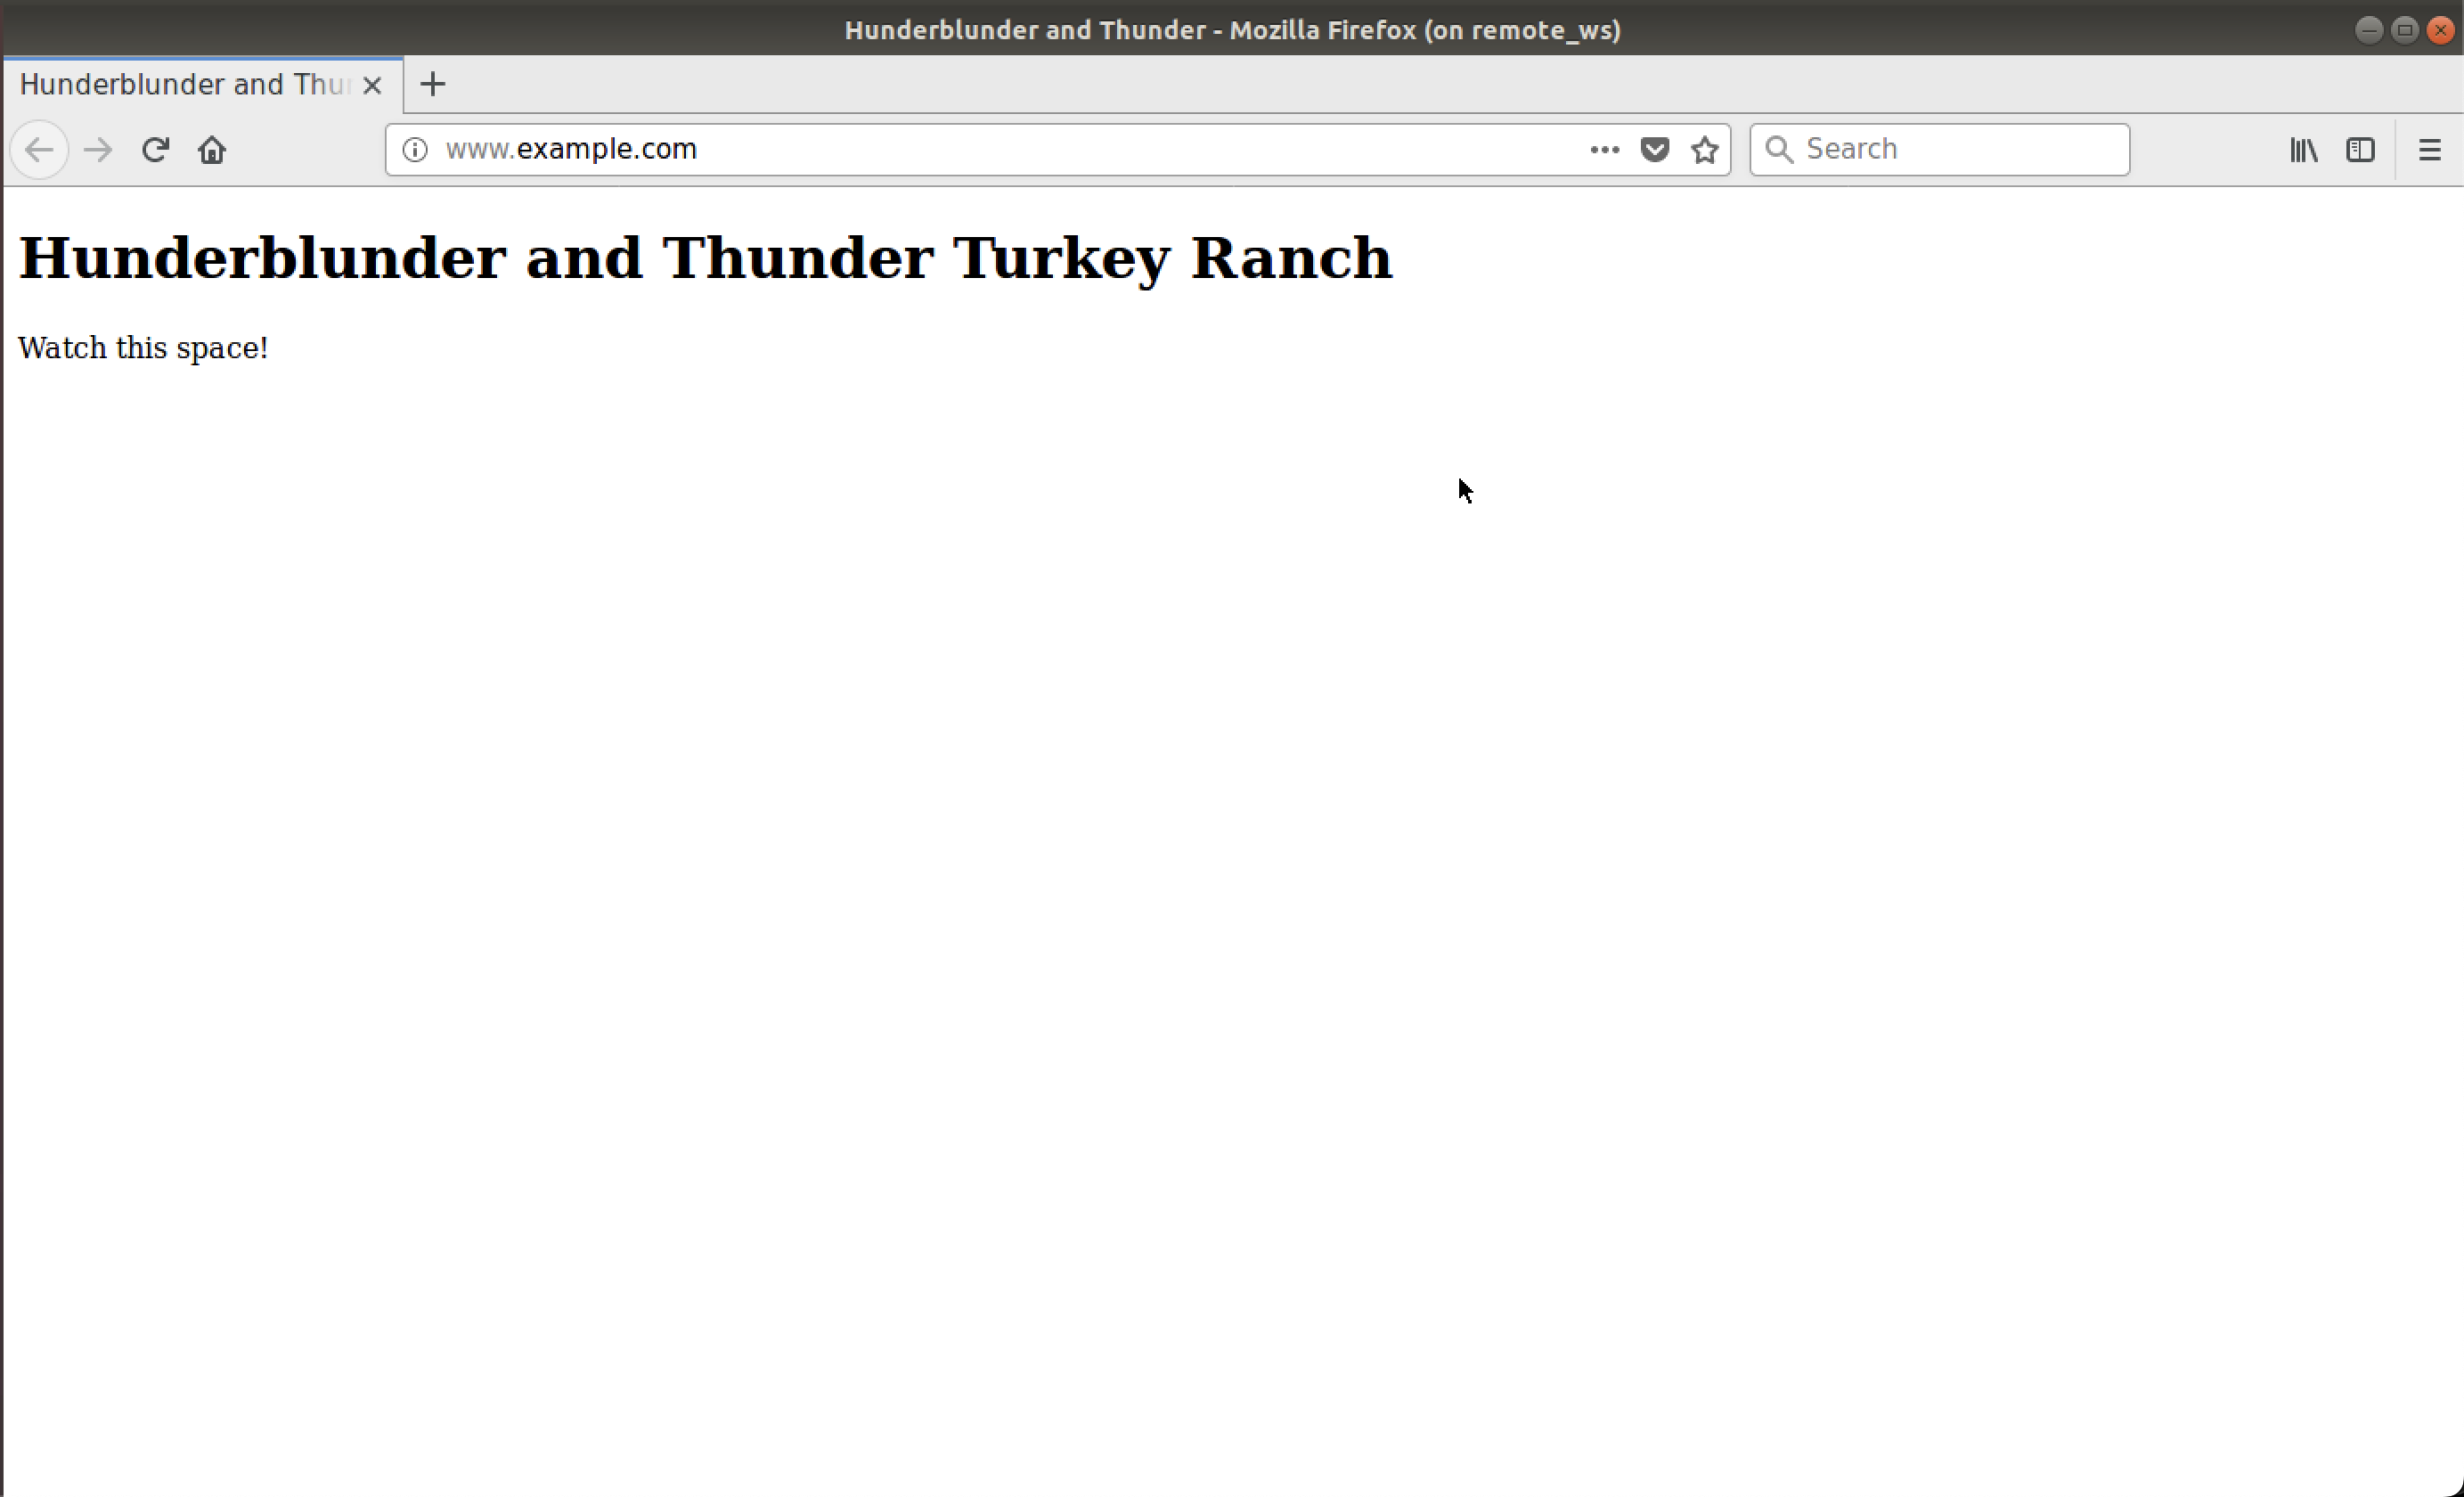
\includegraphics[width=0.7\textwidth]{images/19.png}
    \caption{Firefox Window}
\end{figure}

\subsubsection{Custom Rule for CONFIDENTIAL Traffic}
This task involves creating a specific Snort rule to detect occurrences of the word “CONFIDENTIAL” within network traffic. This simulates monitoring for sensitive information. We add a rule (alert tcp any any -\> any any (msg:”CONFIDENTIAL detected”; content:”CONFIDENTIAL”; sid:00002) to capture traffic containing the keyword “CONFIDENTIAL.” Testing this rule by accessing a page with the specified content confirms that Snort alerts us when sensitive data is transmitted. This task demonstrates how Snort can be configured to monitor specific patterns or keywords, improving its effectiveness in identifying security-related events.\\
So, we use the command below to add a new rule to our test:
\[\texttt{(msg:”CONFIDENTIAL detected”; content:”CONFIDENTIAL”; sid:00002;)}\]

\begin{figure}[h!]
    \centering
    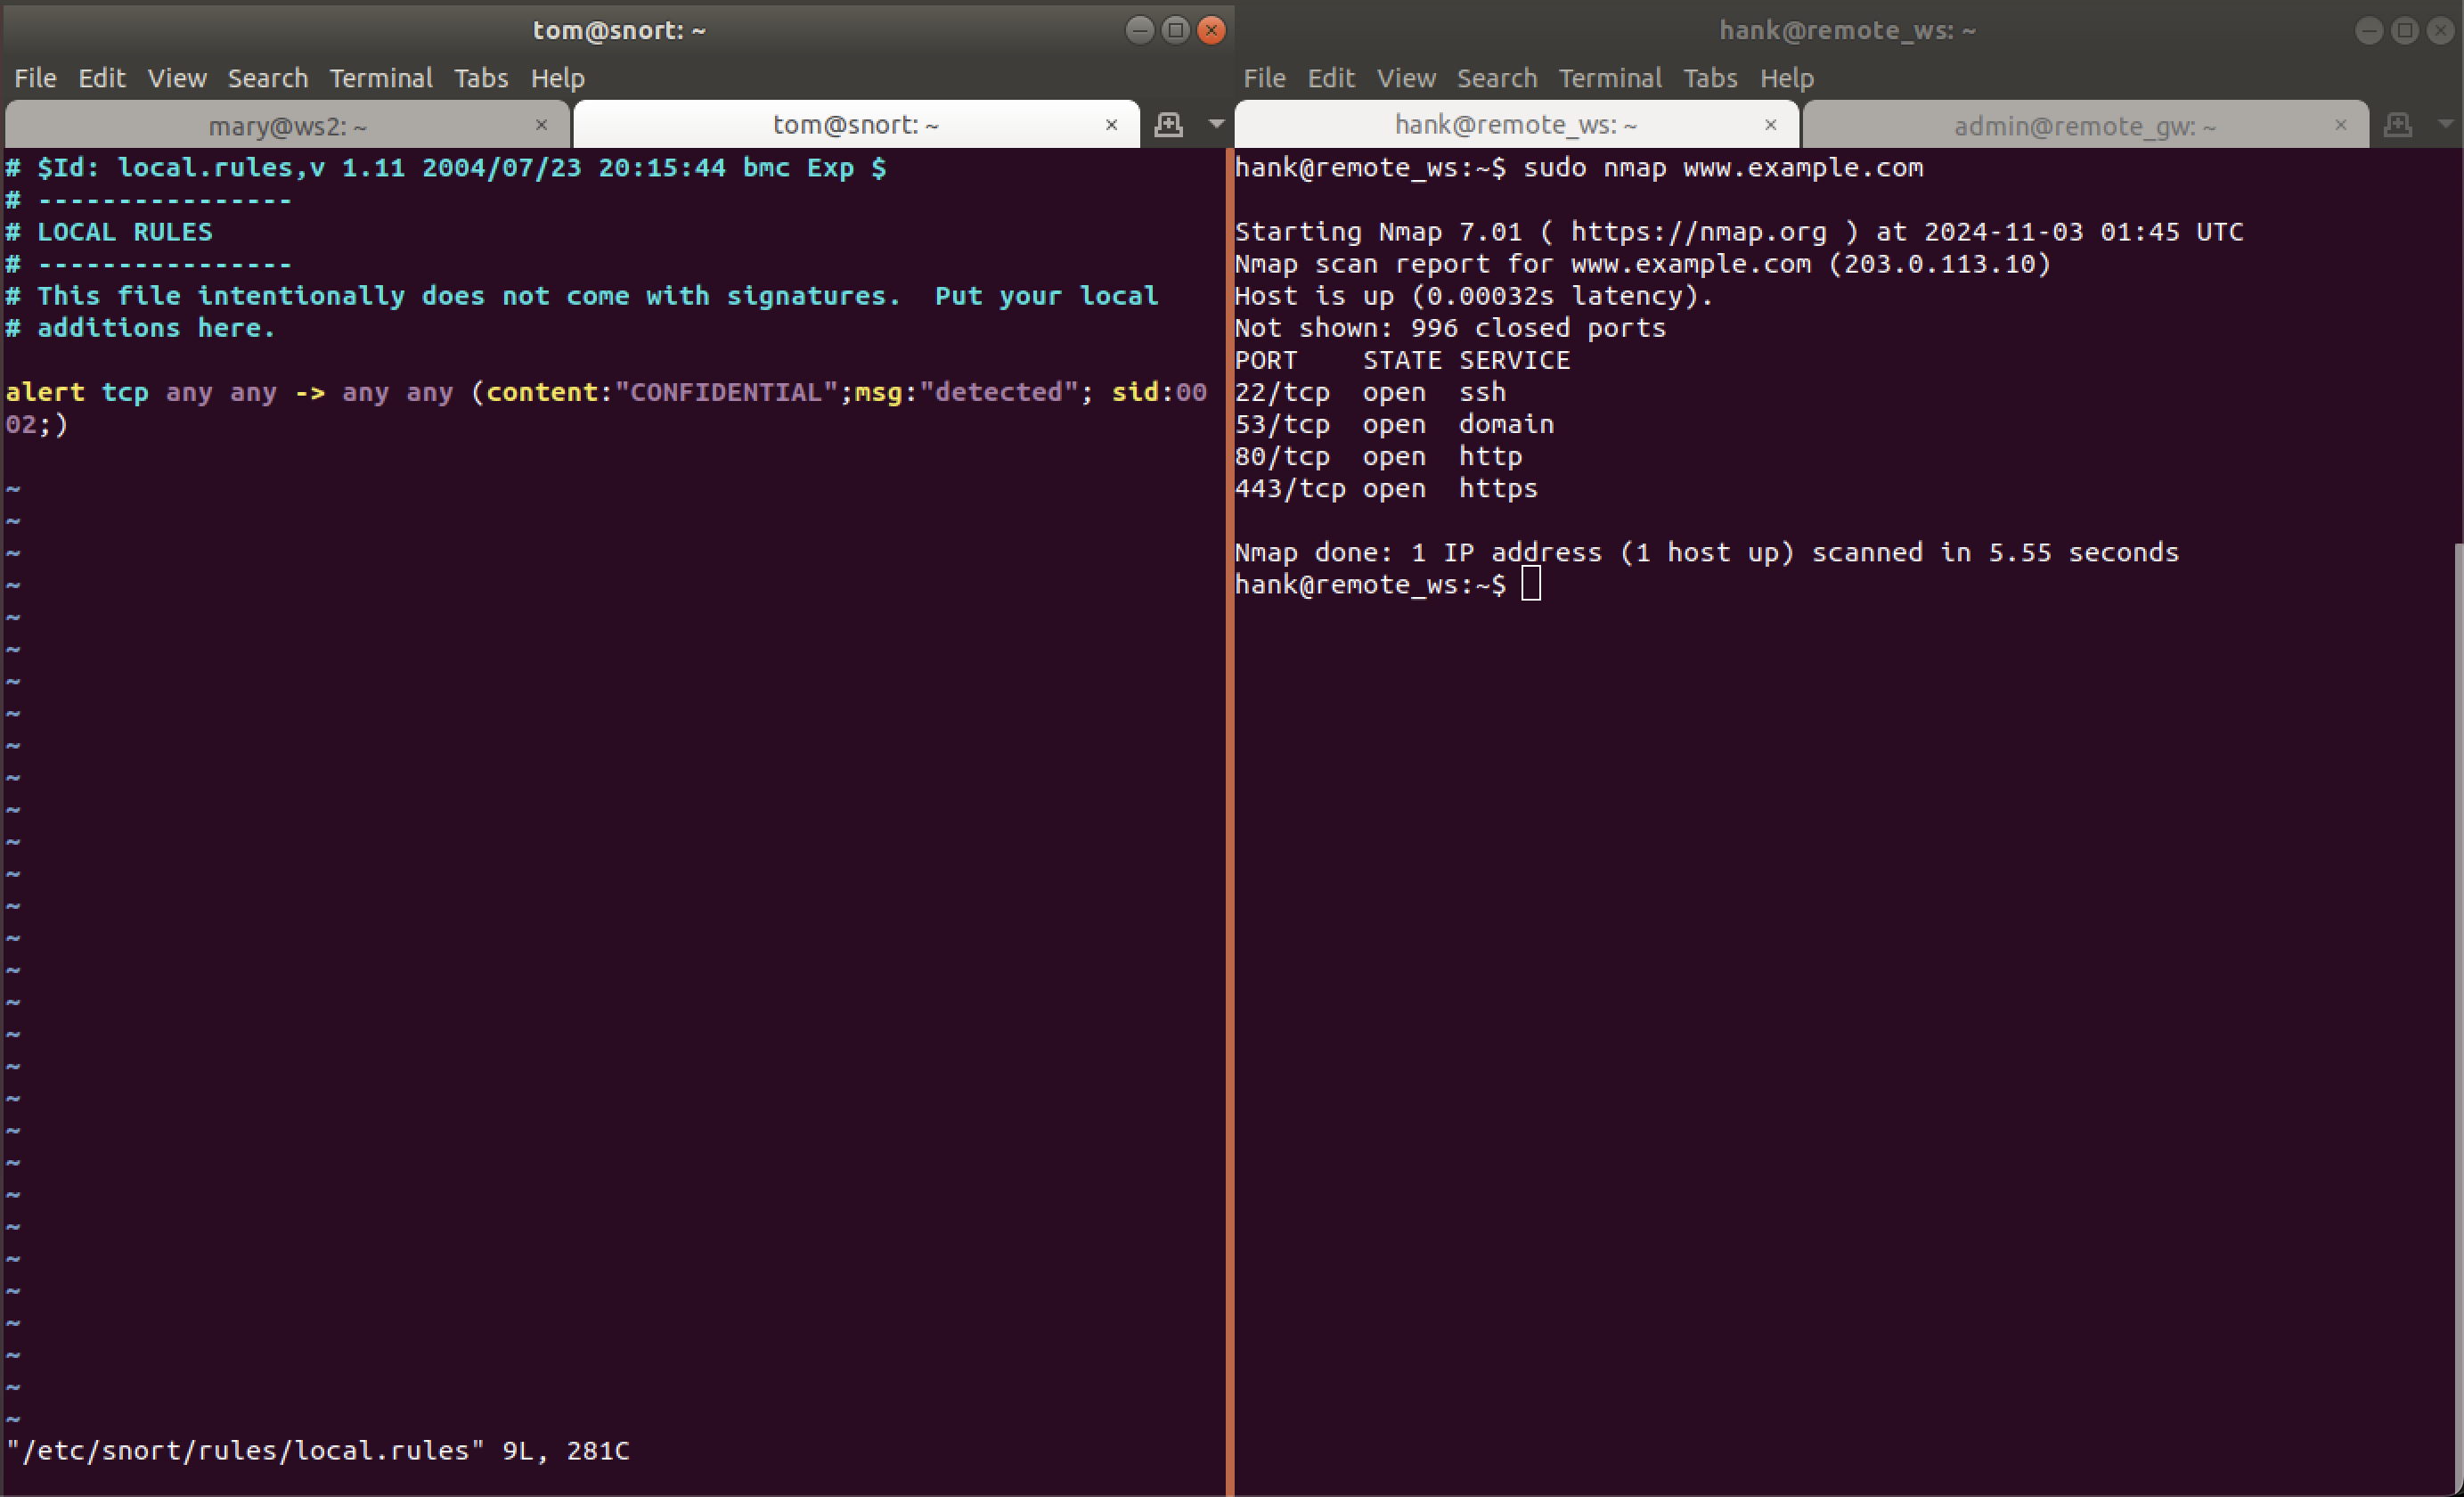
\includegraphics[width=0.7\textwidth]{images/20.png}
    \caption{New Rule}
\end{figure}
Again, we restart the \texttt{./start\_snort.sh} and use \texttt{firefox www.example.com/plan.html}:

\break

\begin{figure}[h!]
    \centering
    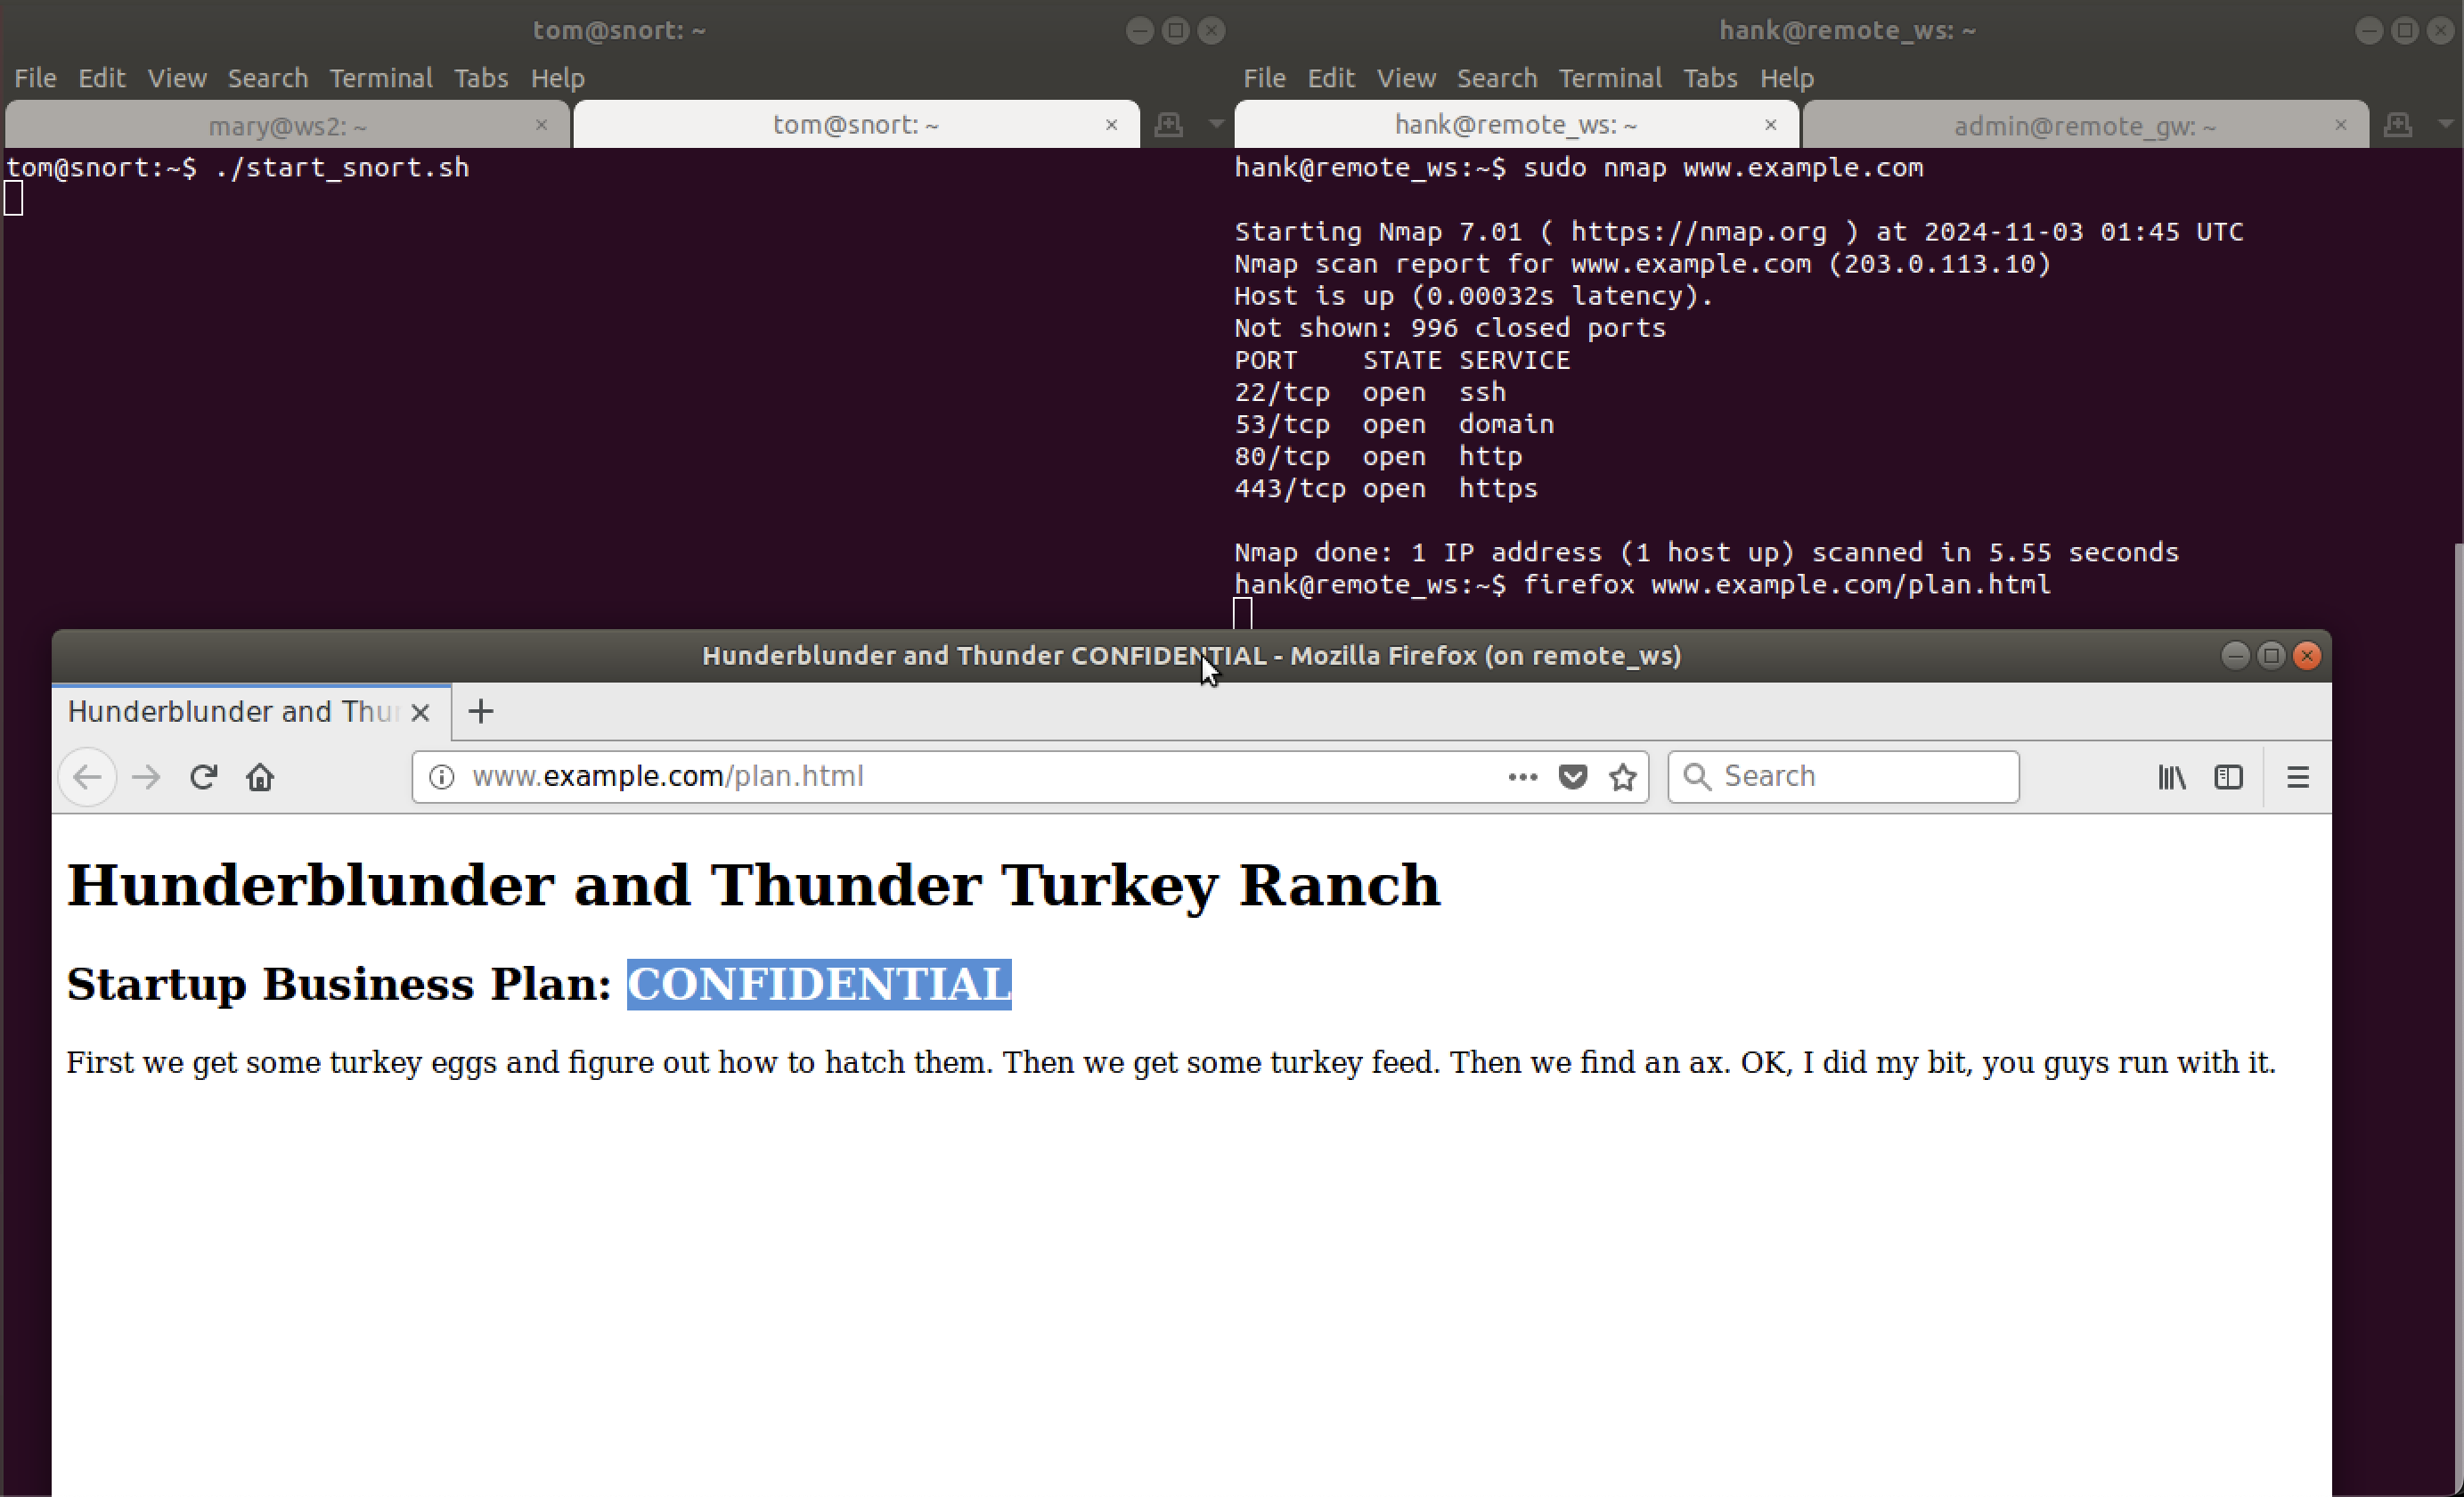
\includegraphics[width=0.7\textwidth]{images/21.png}
    \caption{Confidential Test}
\end{figure}

We test this by accessing the “CONFIDENTIAL” page over HTTPS, using SSL encryption. Since Snort cannot decrypt SSL traffic, it is unable to generate an alert when monitoring encrypted sessions. This task highlights a key limitation in Snort’s detection capabilities with encrypted data, as it lacks visibility into encrypted payloads. The exercise introduces the concept of using a reverse proxy to decrypt traffic before it reaches Snort, which would allow Snort to inspect the contents of encrypted traffic in environments where such monitoring is necessary.

\subsubsection{Watching Internal Traffic}
Here, we configure Snort to monitor internal traffic by mirroring data from specific internal IP addresses to the Snort interface. Running an nmap scan from an internal workstation (such as Mary’s workstation) tests Snort’s ability to detect internal network scans. If Snort fails to capture this activity, we modify the /etc/rc.local script on the gateway to mirror traffic from the internal IP to Snort. Once Snort is restarted, we rerun the scan to confirm that alerts are generated for internal traffic. This task illustrates how to expand Snort’s coverage to monitor internal network activity, which is crucial for comprehensive network security.\\
After we use \texttt{sudo nmap www.example.com} in \textbf{mary@ws2}, we can note that its not possible to find \texttt{ICMP PING NMAP}, once this snort is not available to navigate between internal services.\\
To solve that problem, we can edit the \texttt{iptables} file in the ubuntu directory, and, after that, we reload the test in mary's terminal.

\begin{figure}[h!]
    \centering
    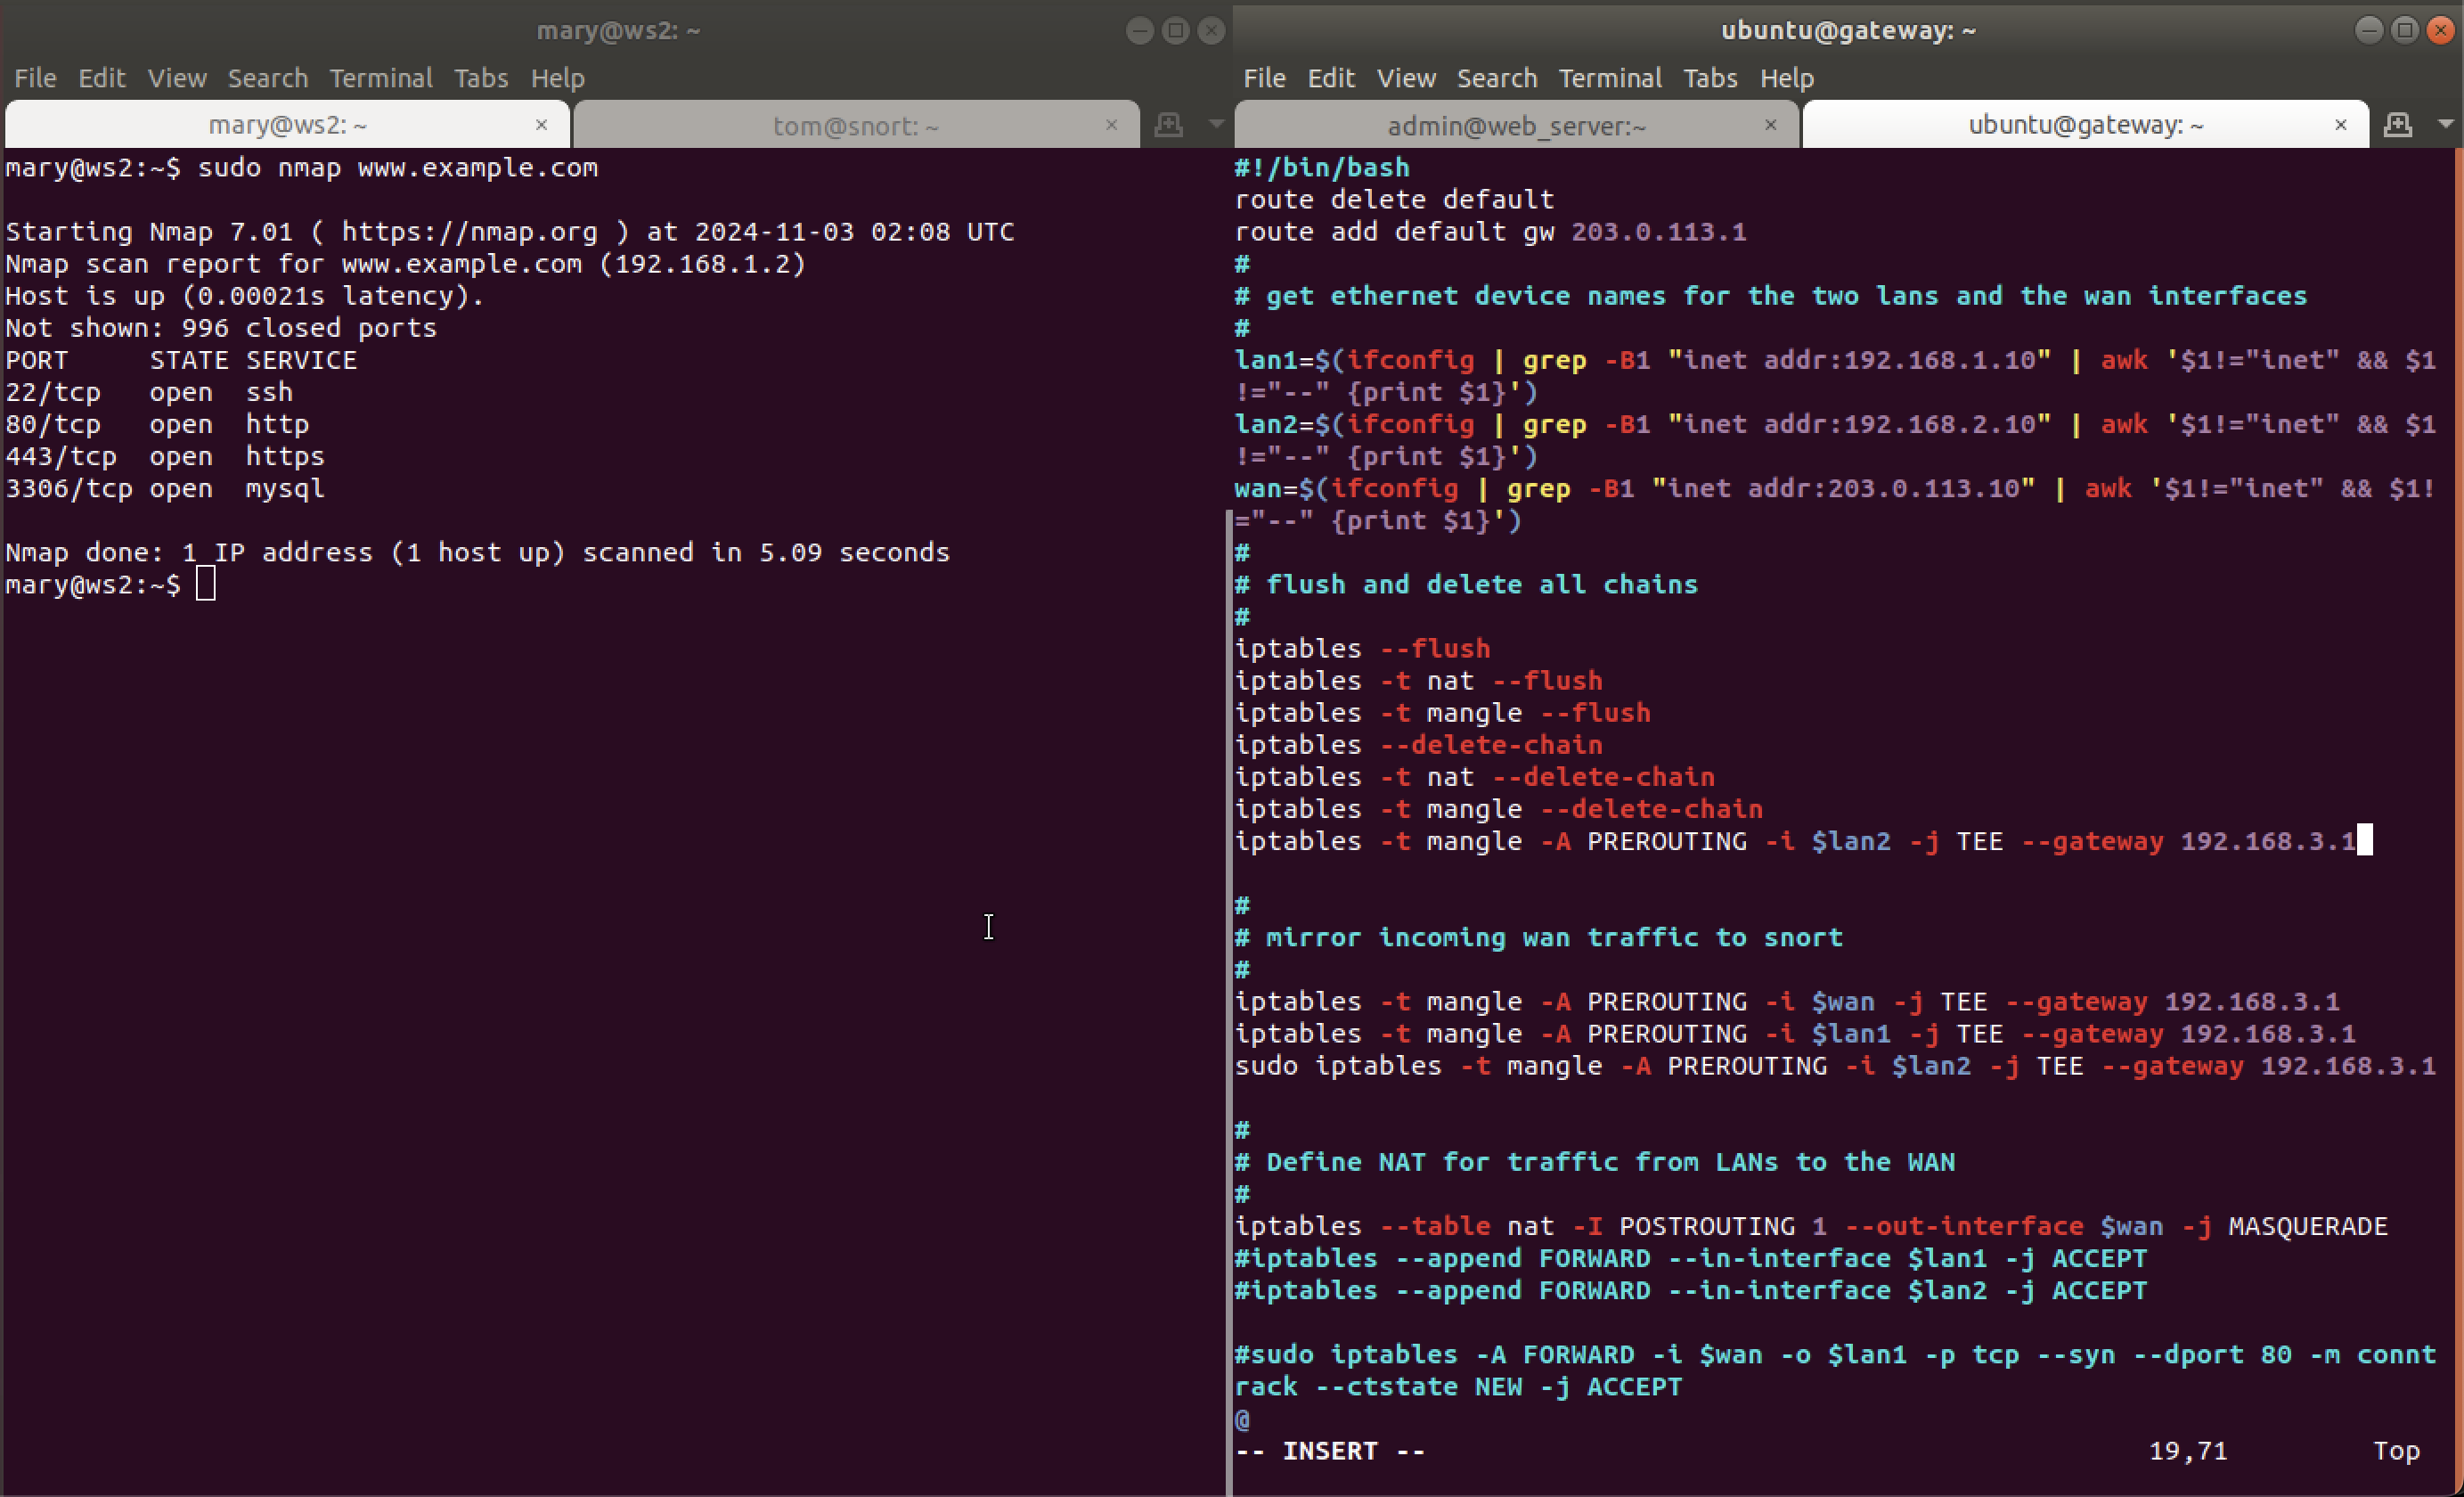
\includegraphics[width=0.5\textwidth]{images/22.png}
    \caption{Iptables Edit}
\end{figure}

\break 

\begin{figure}[h!]
    \centering
    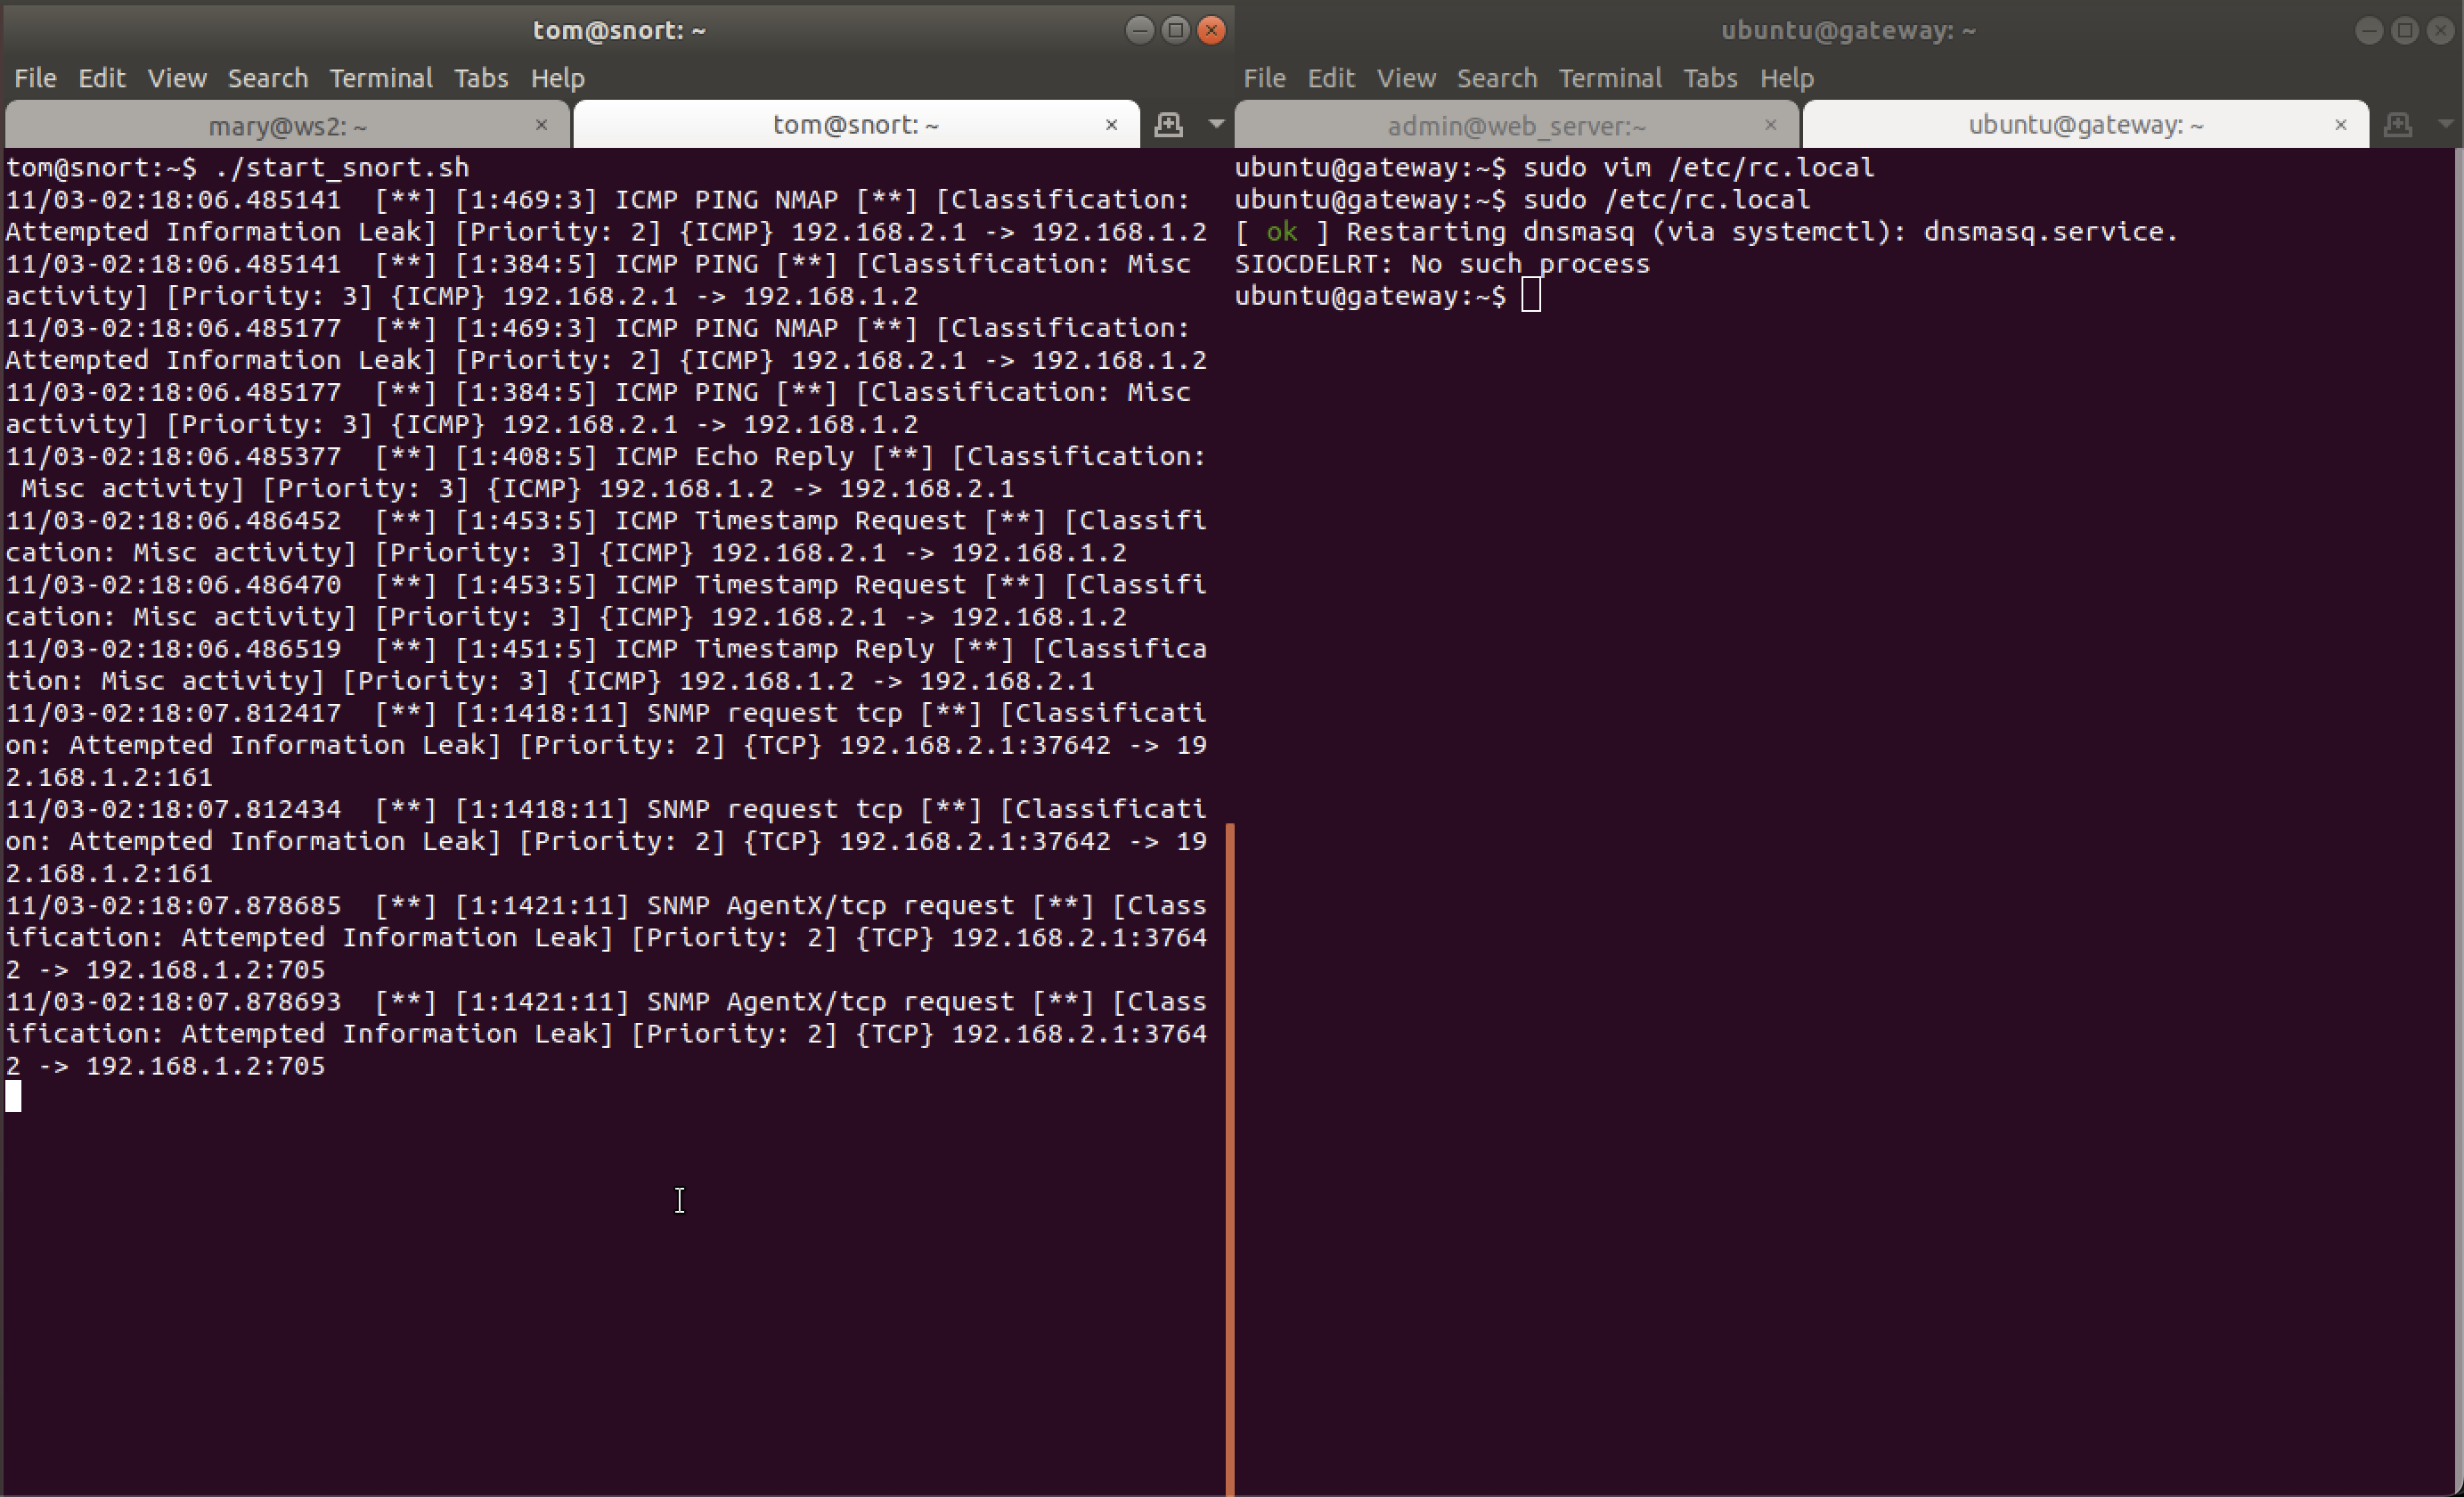
\includegraphics[width=0.7\textwidth]{images/23.png}
    \caption{Mary's Test}
\end{figure}

\subsubsection{Distinguishing Traffic by Address}
In the final task, we configure Snort to differentiate between internal and external traffic. By modifying the rule to trigger alerts only when external sources attempt to access sensitive content, we reduce false positives for internal access. We update the rule (alert tcp !\$HOME\_NET any -\> \$HOME\_NET any (msg:"External access to CONFIDENTIAL data"; content:"CONFIDENTIAL"; sid:00002;)) to limit alerts to external traffic, allowing internal access without triggering unnecessary alerts. This task demonstrates Snort’s flexibility in creating targeted rules to improve alert relevance, which is essential for maintaining an effective intrusion detection system.
For this, we can add a new rule:

\begin{figure}[h!]
    \centering
    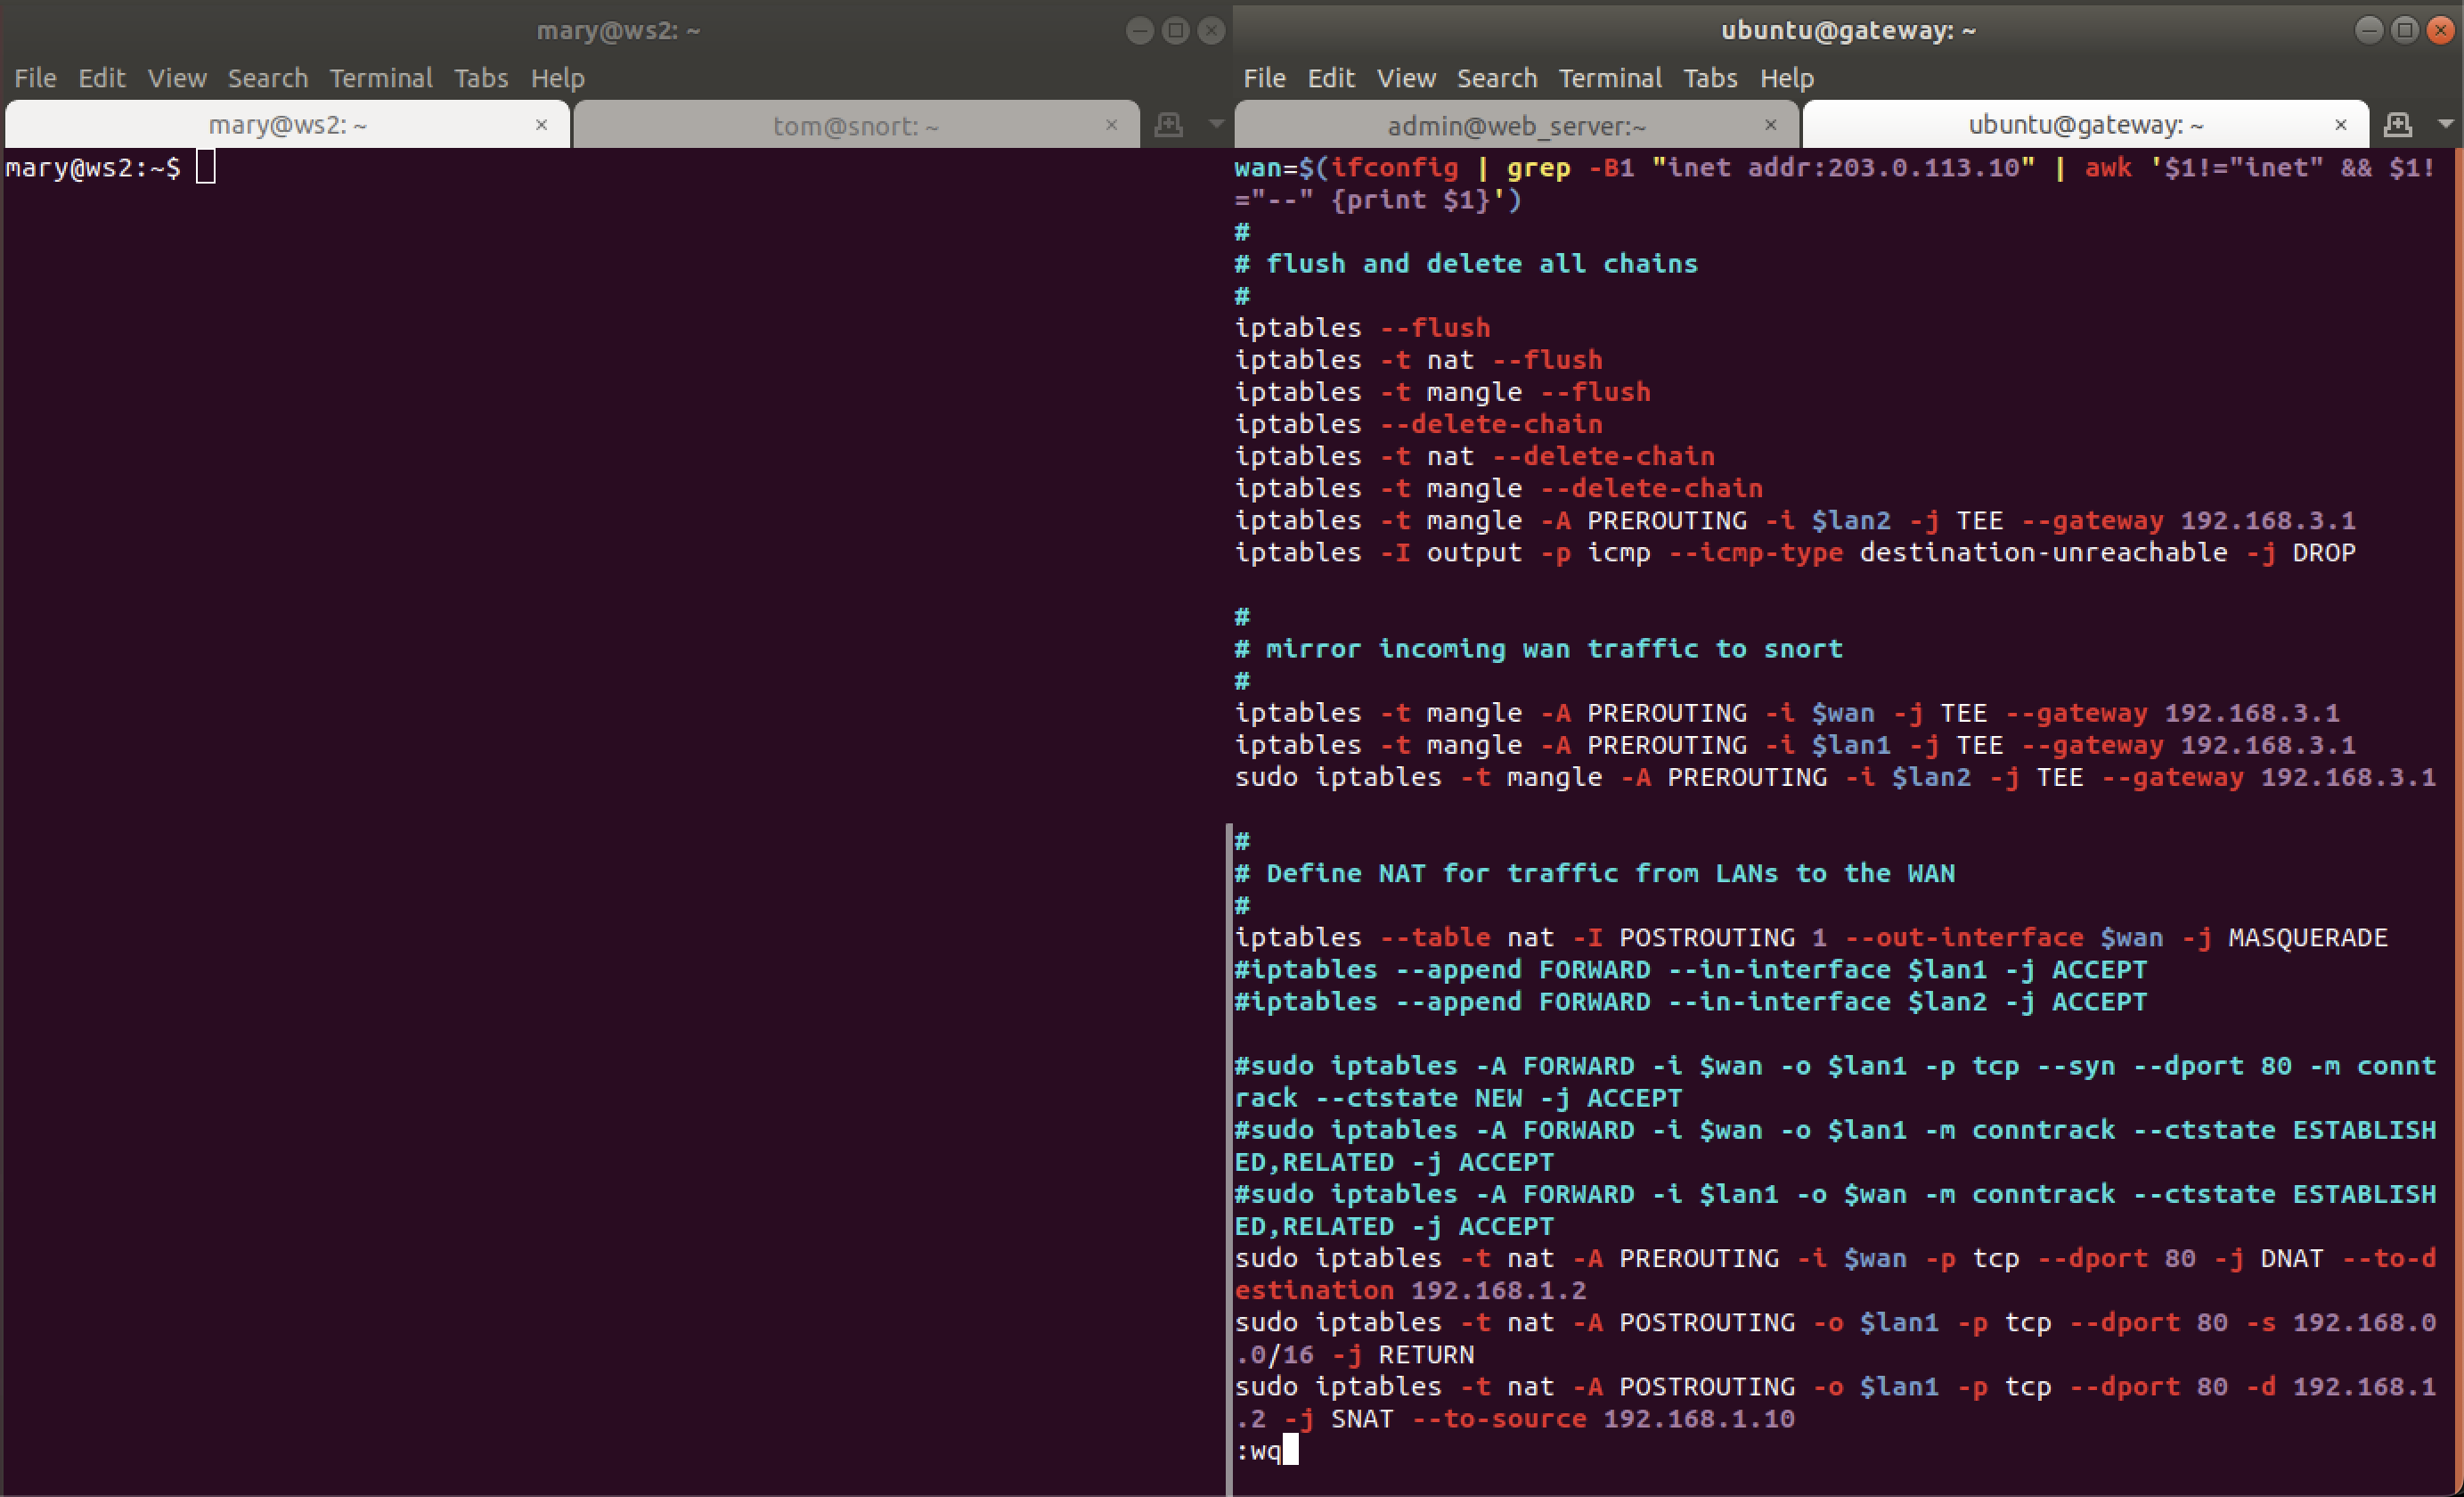
\includegraphics[width=0.7\textwidth]{images/24.png}
    \caption{New Rule}
\end{figure}

\break

\begin{figure}[h!]
    \centering
    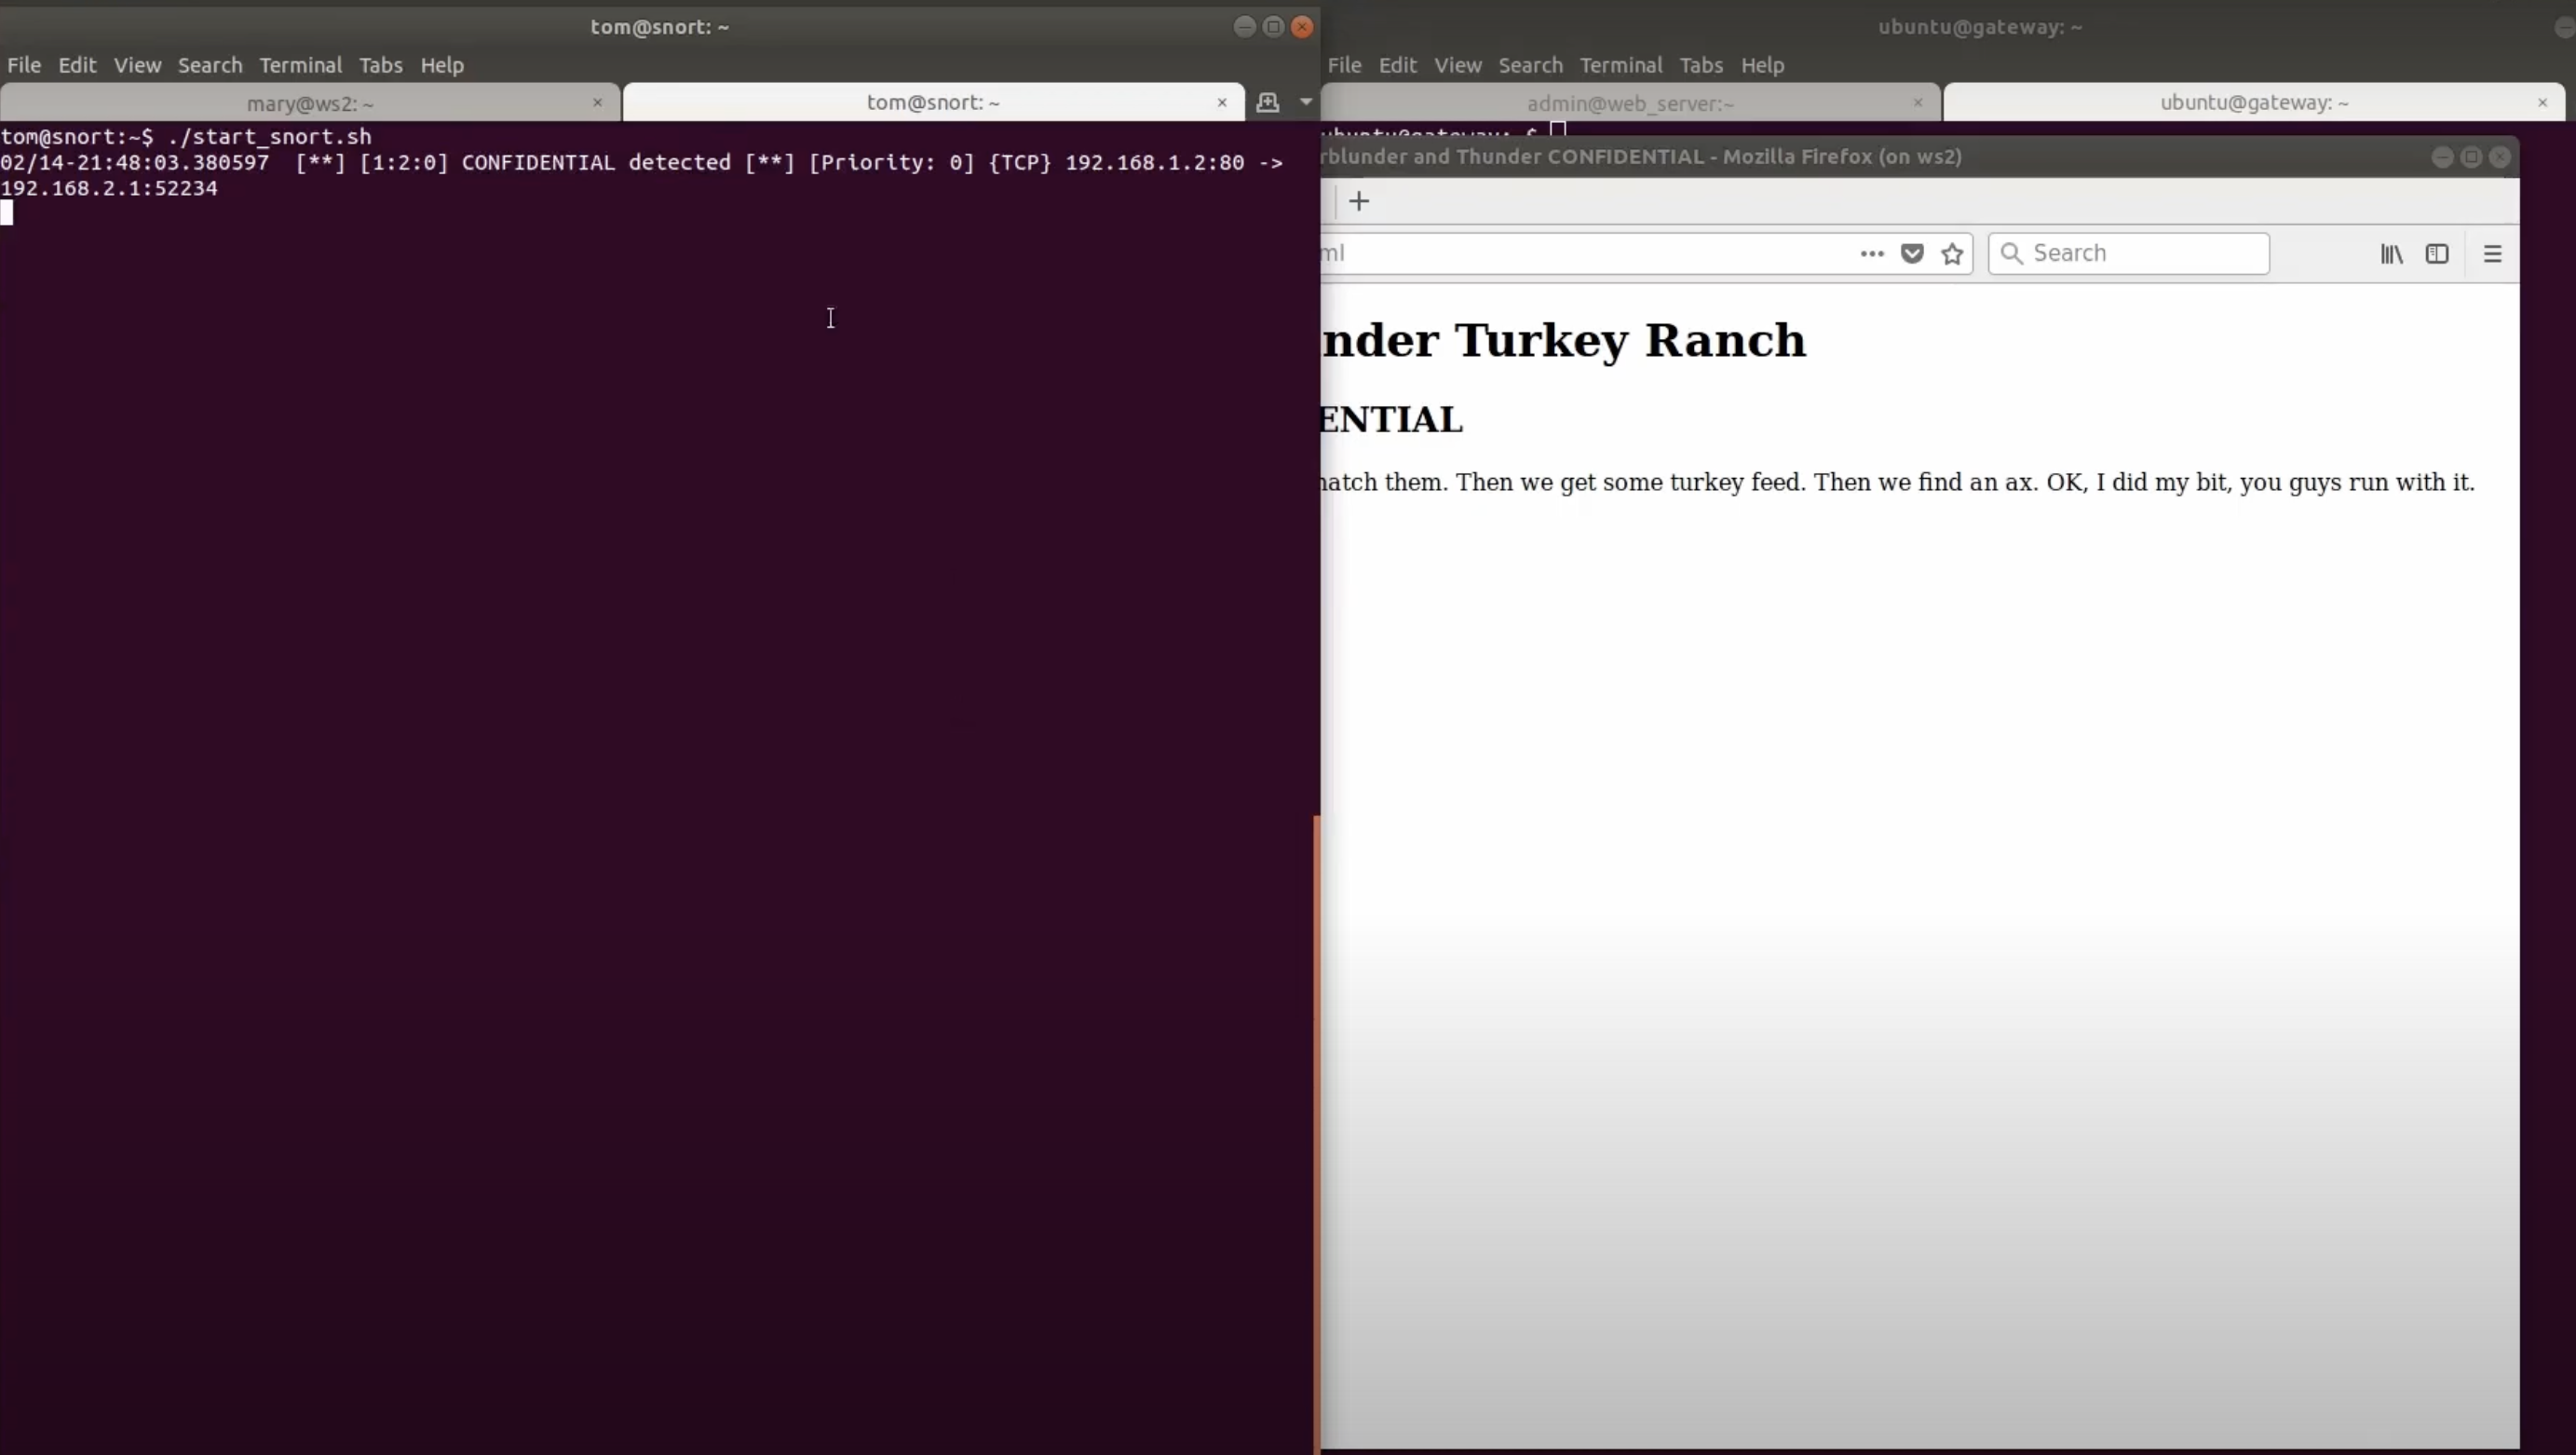
\includegraphics[width=0.7\textwidth]{images/25.png}
    \caption{New Rule Confirmation}
\end{figure}

After that, we can adjust the rule to detect wich user is connected:

\begin{figure}[h!]
    \centering
    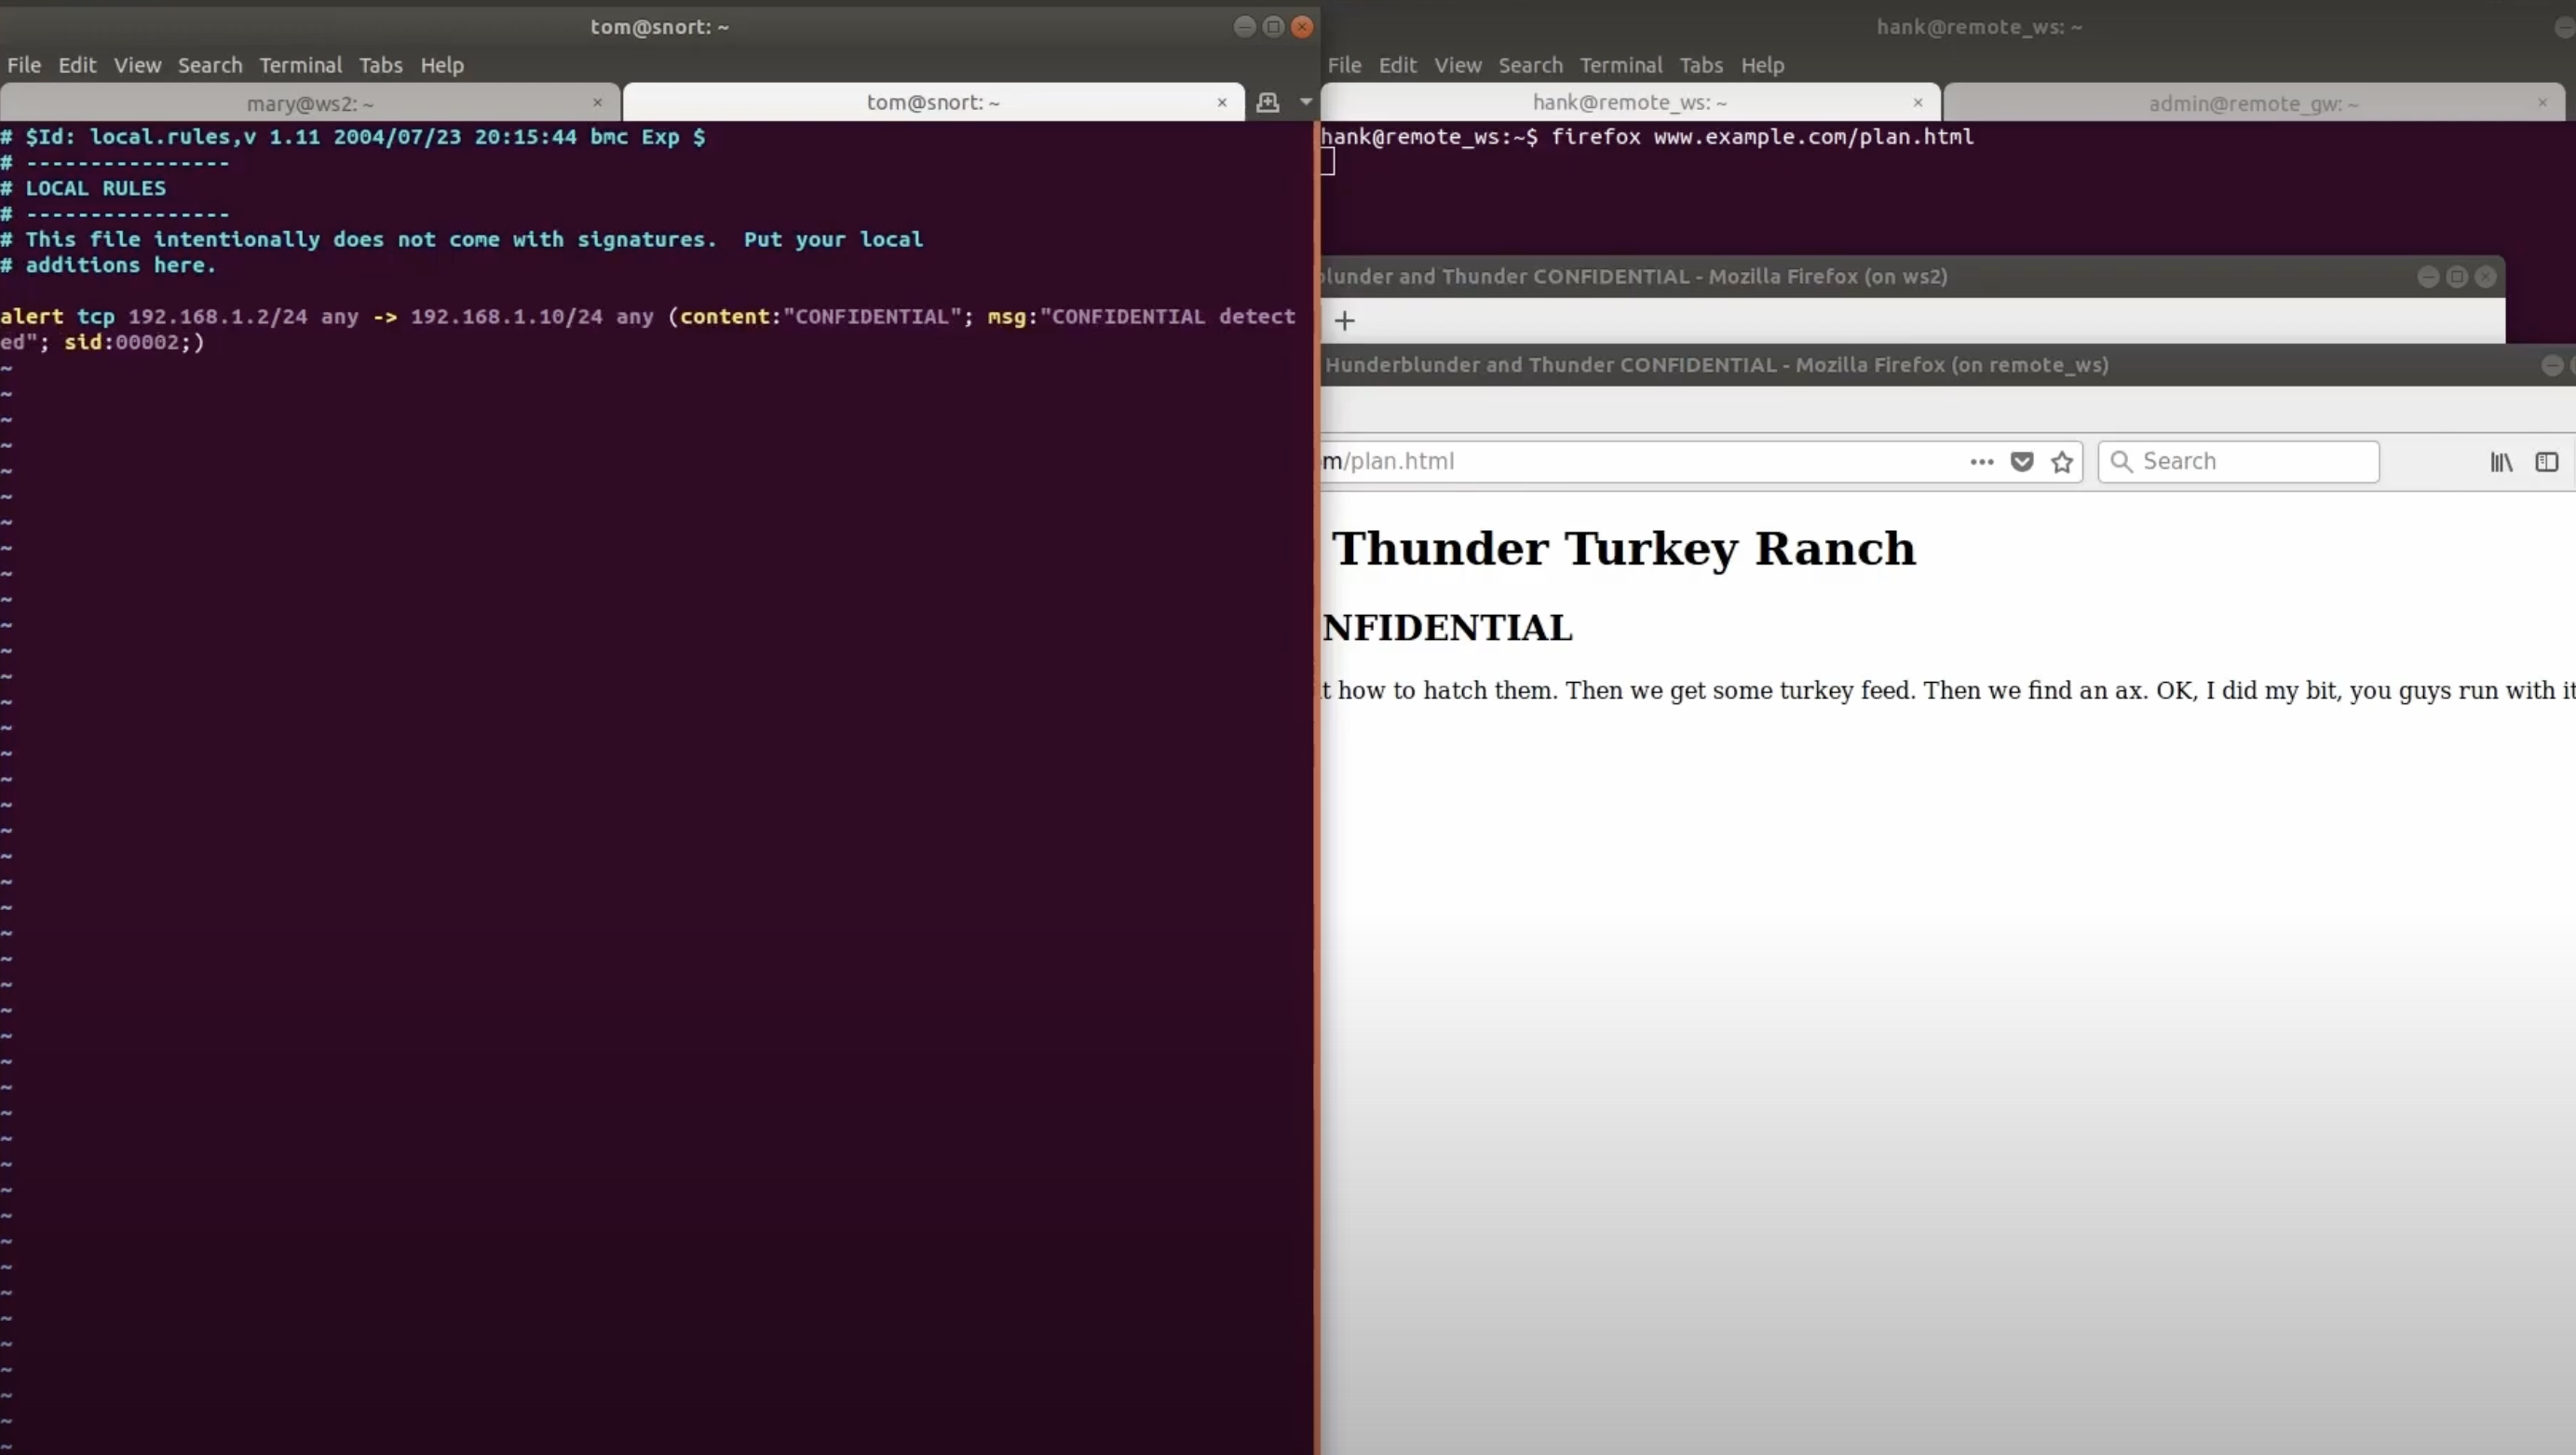
\includegraphics[width=0.7\textwidth]{images/26.png}
    \caption{Rule Adjust}
\end{figure}

\break

\begin{figure}[h!]
    \centering
    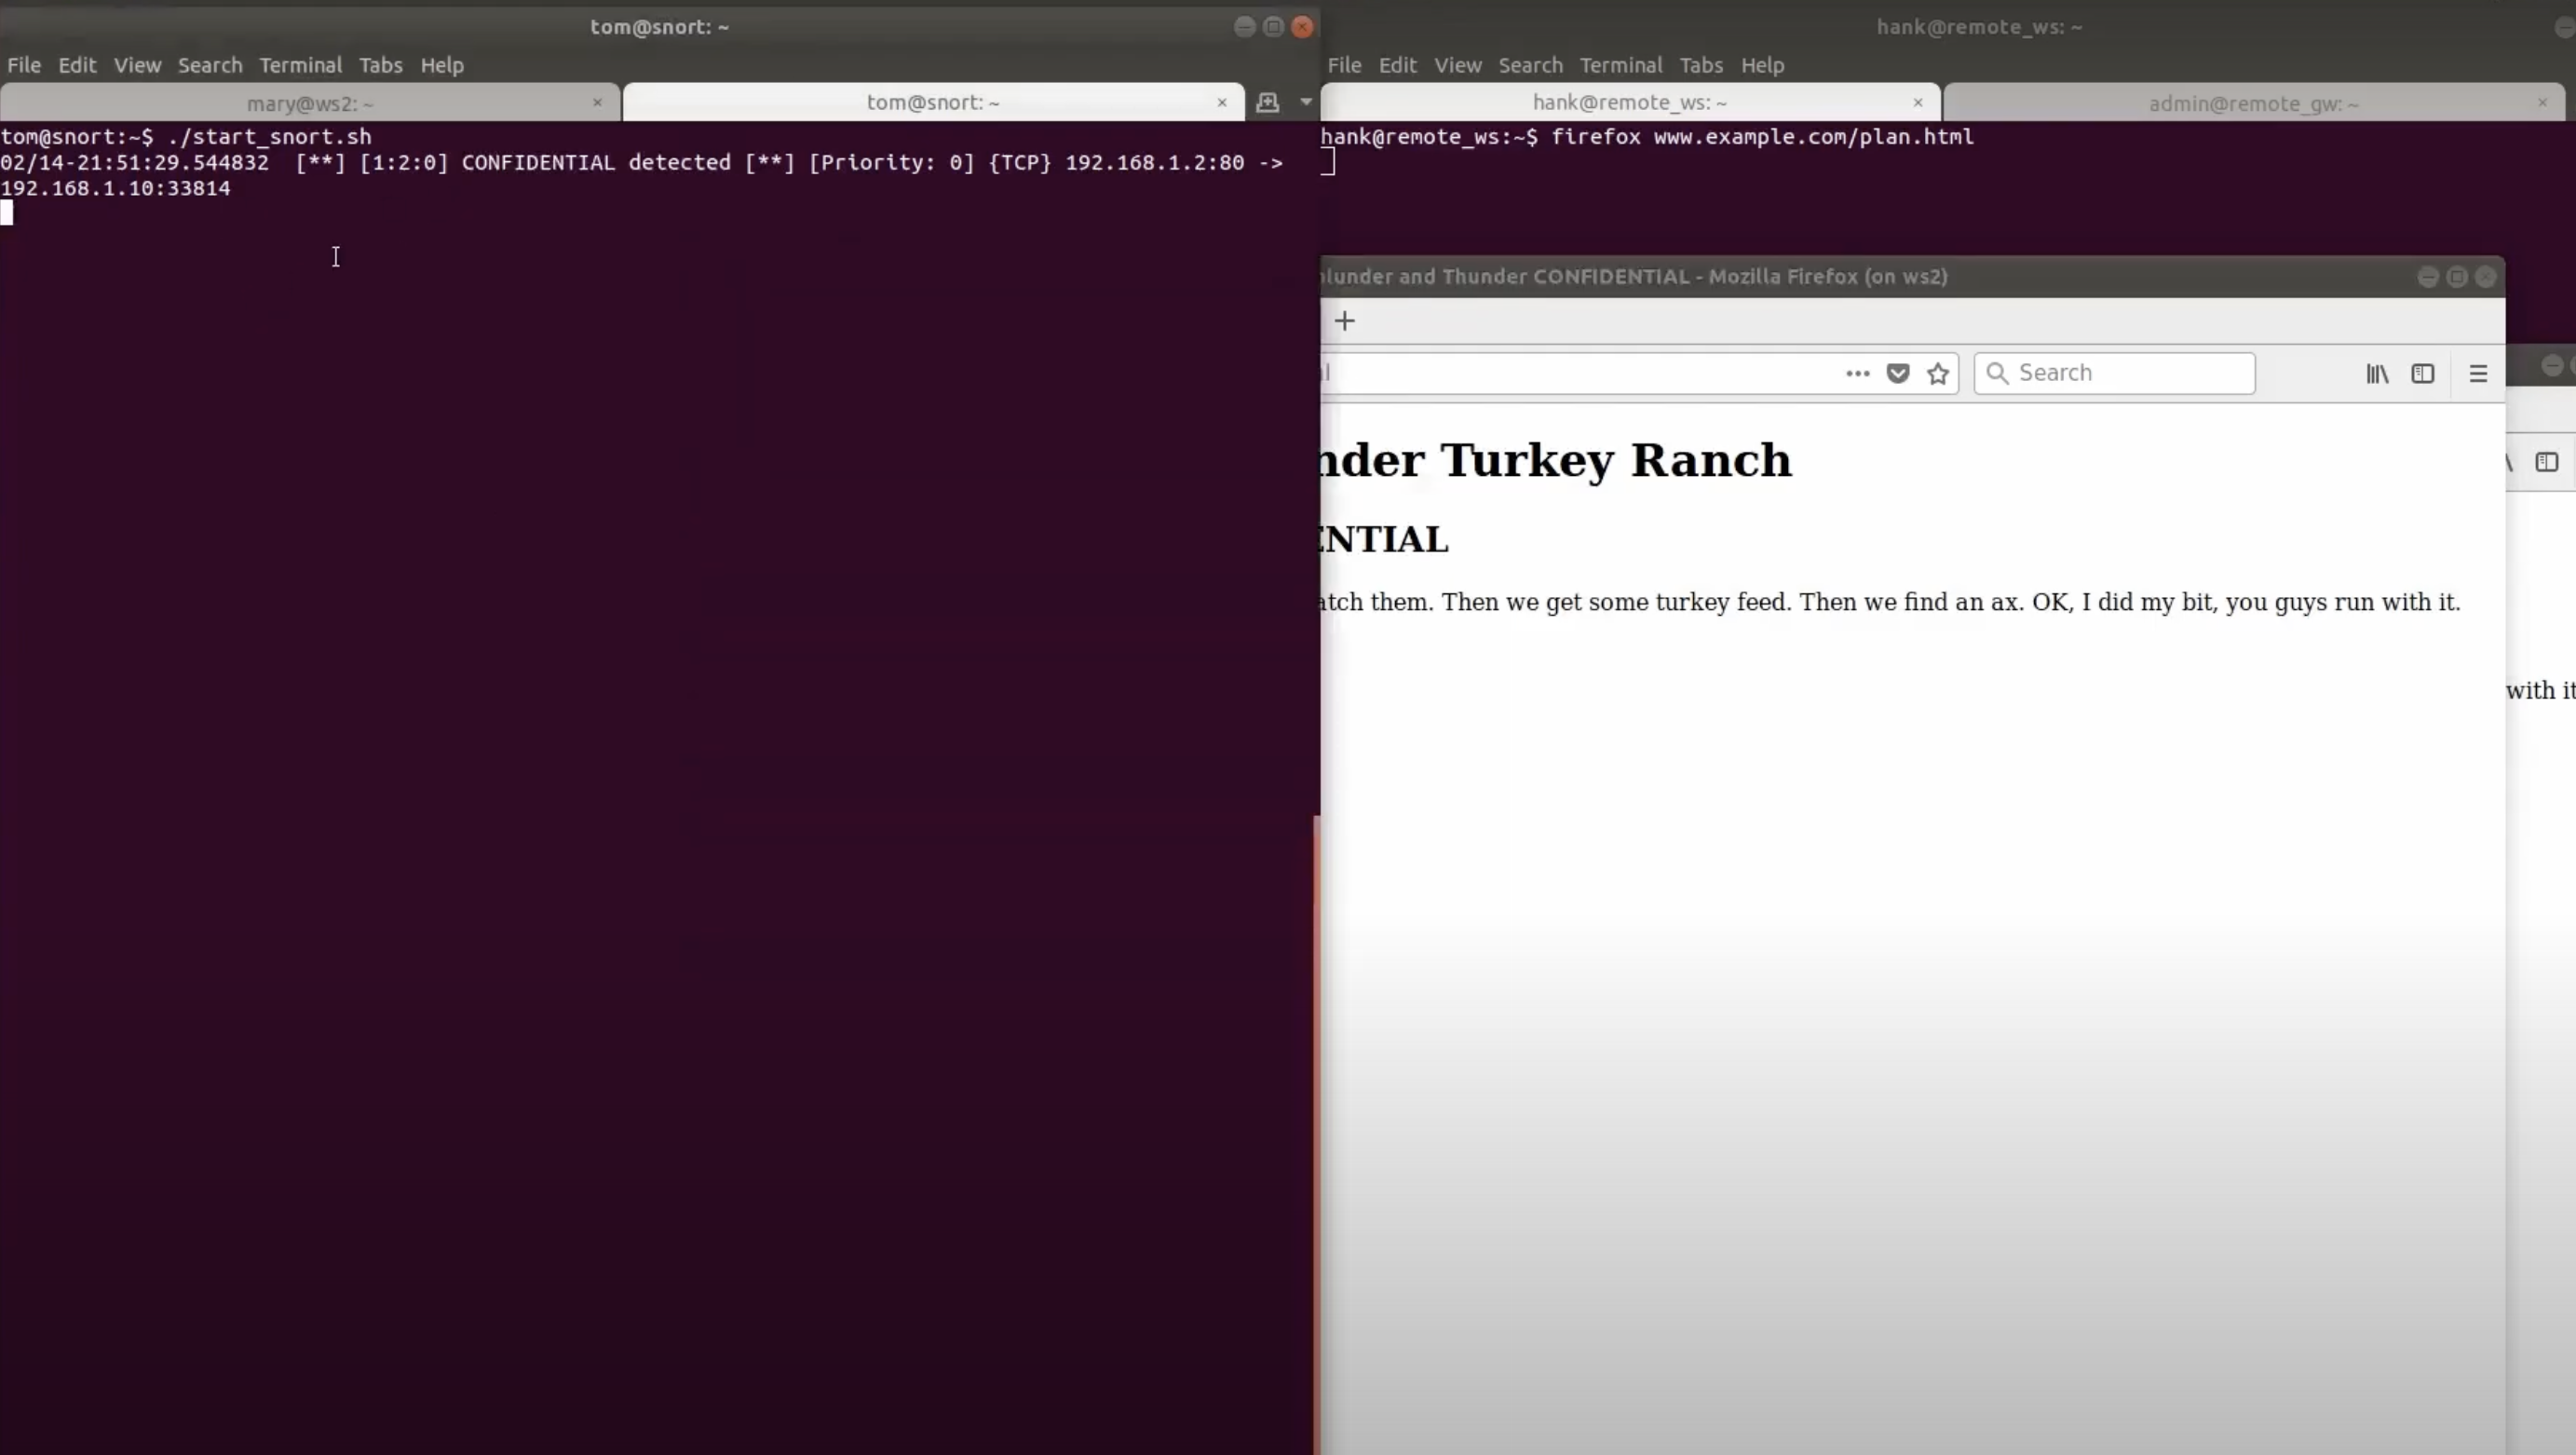
\includegraphics[width=0.7\textwidth]{images/27.png}
    \caption{Rule Test}
\end{figure}

\begin{figure}[h!]
    \centering
    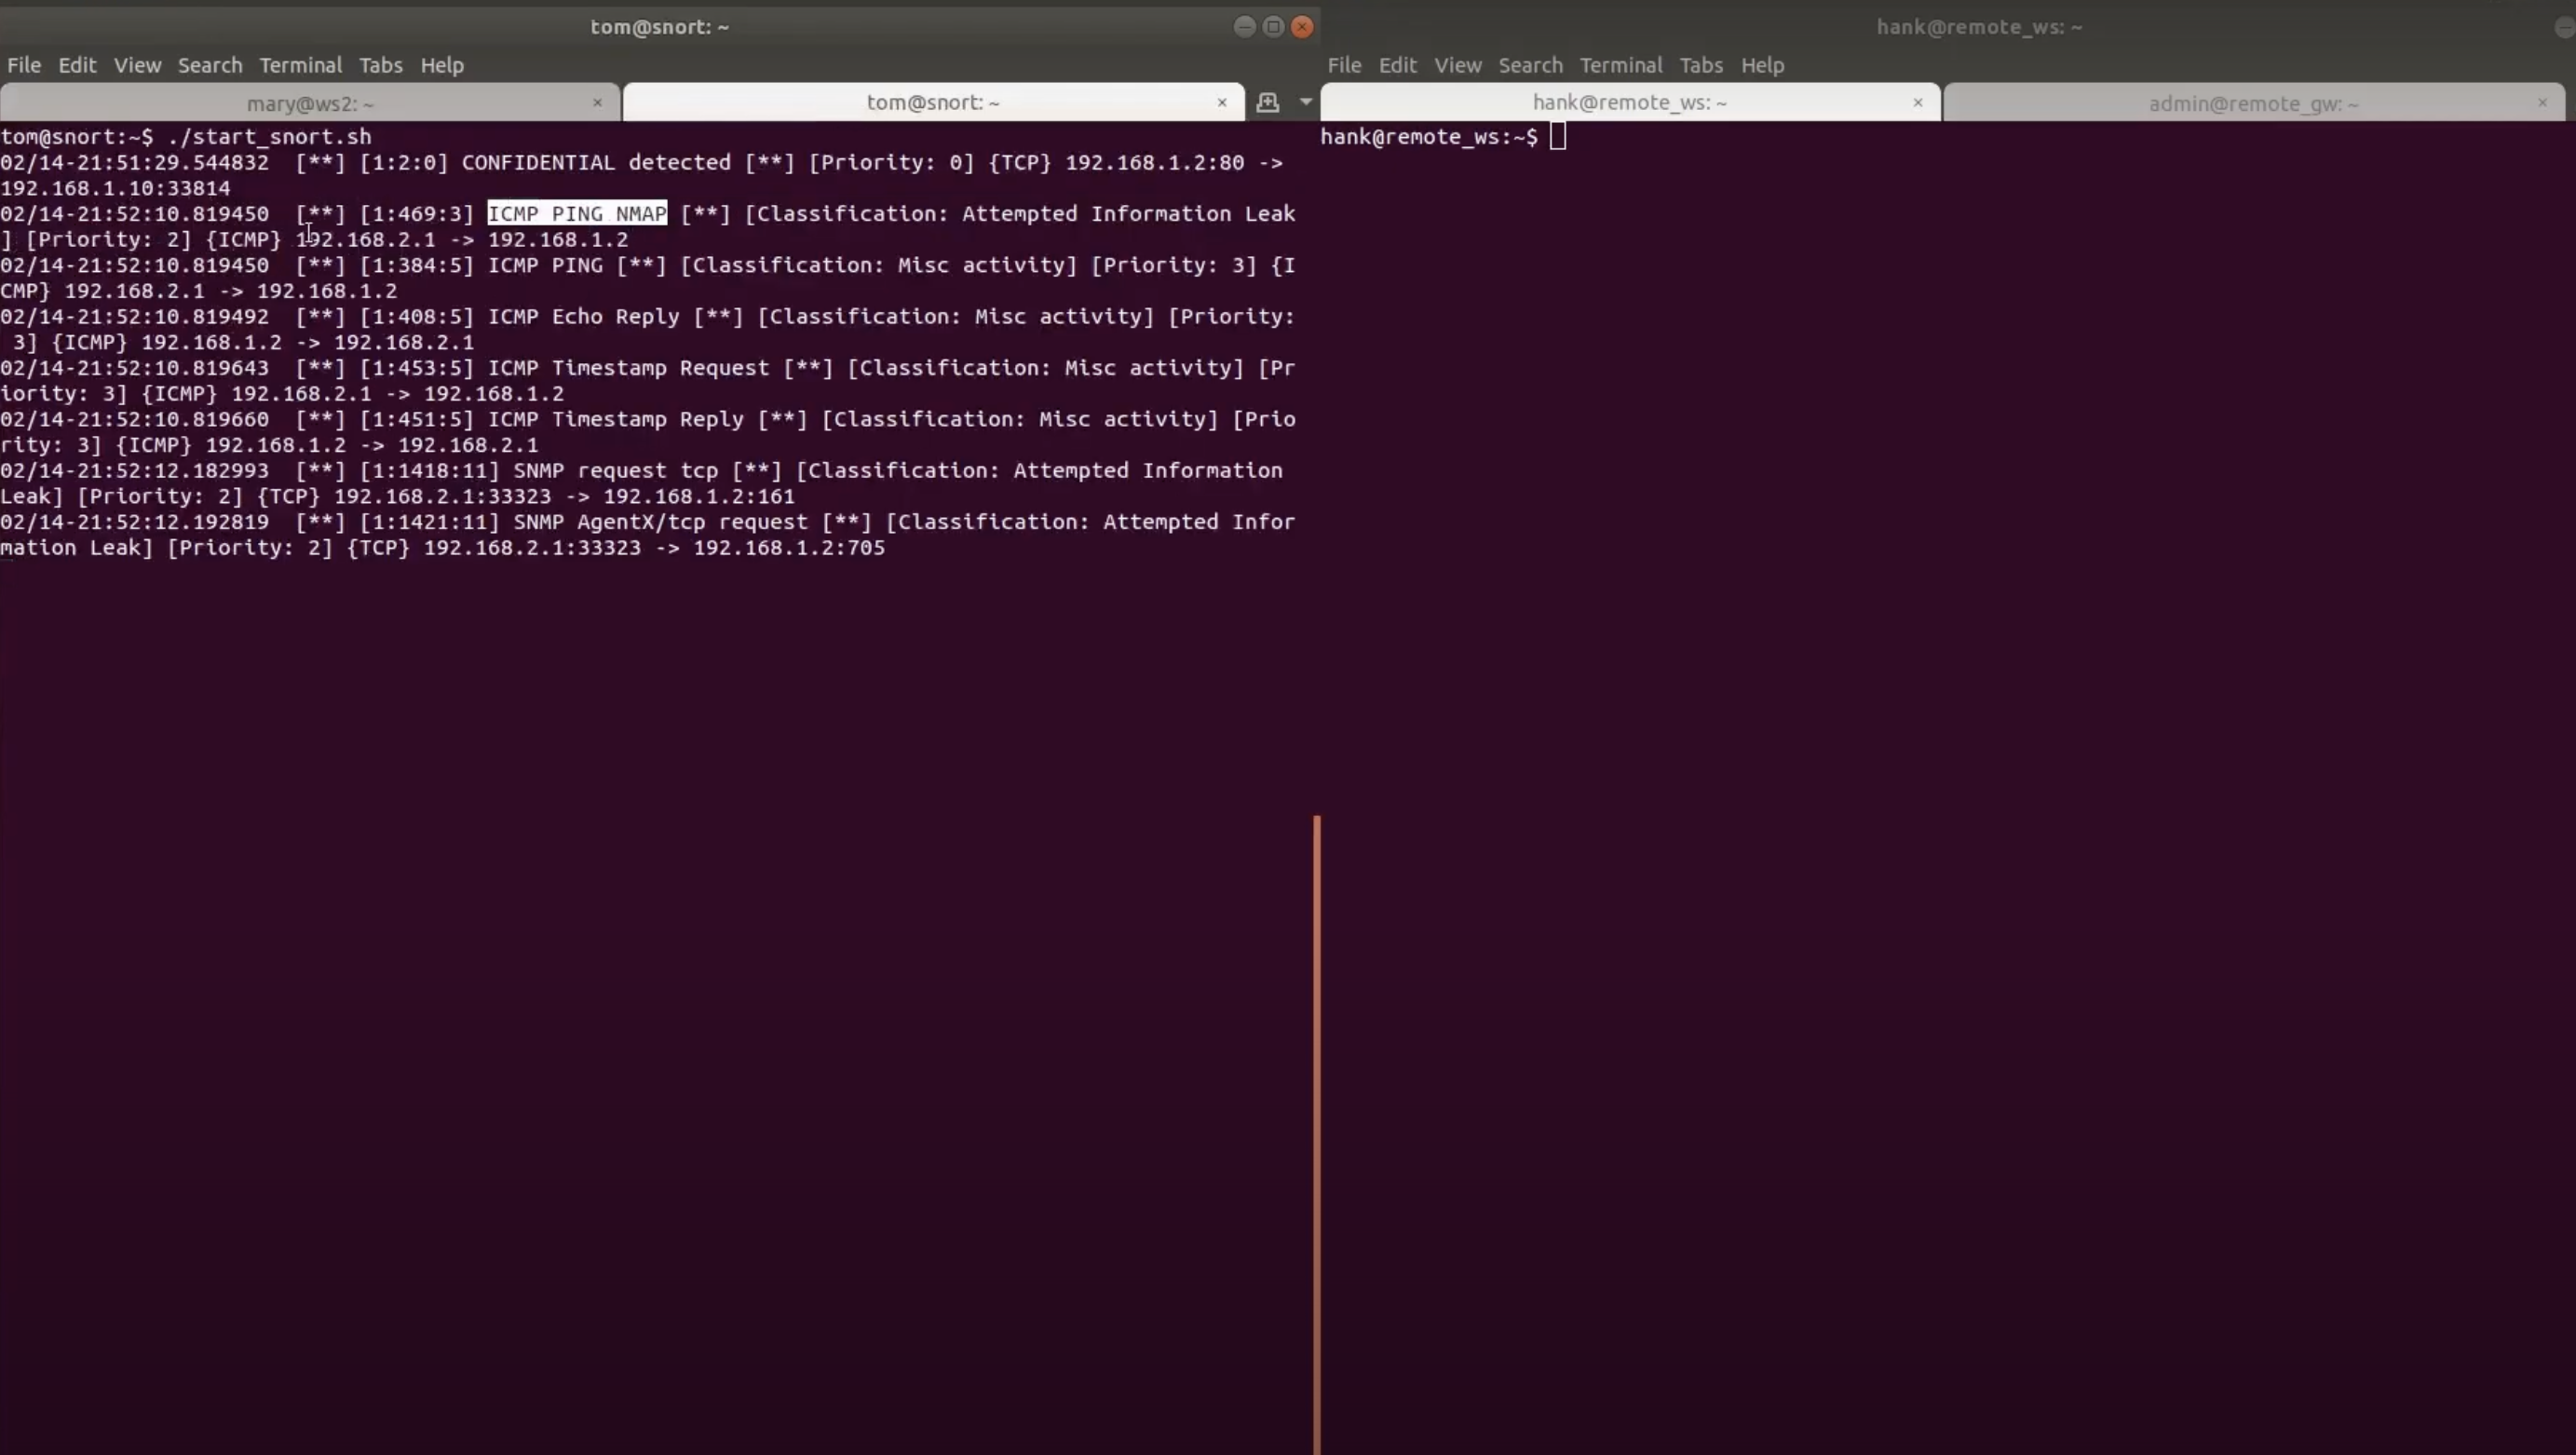
\includegraphics[width=0.7\textwidth]{images/28.png}
    \caption{PING Test}
\end{figure}

\subsection{Conclusion}
This Snort lab provided valuable hands-on experience in configuring and operating a network intrusion detection system. Through practical exercises, we explored the basics of Snort’s alerting capabilities, from running pre-configured rules to creating custom rules for targeted monitoring. By crafting and testing specific rules, we observed how overly broad criteria can overwhelm the alert system, while carefully tailored rules significantly improve Snort’s effectiveness.

We also examined Snort’s limitations in handling encrypted traffic, highlighting the need for complementary tools, such as reverse proxies, when monitoring encrypted communications. Additionally, configuring Snort to monitor both internal and external network traffic allowed us to understand the importance of customizing alerts based on traffic source, enhancing the relevance of detected threats and reducing false positives.

Overall, this lab reinforced critical concepts in network security, including the importance of specificity in rule creation, handling encrypted traffic, and distinguishing internal from external threats. By applying these principles, we gained a deeper understanding of how to use Snort effectively to detect and mitigate potential security breaches, preparing us for real-world applications of intrusion detection and prevention systems.

\end{document}